% Lines starting with a percent sign (%) are comments. LaTeX will 
% not process those lines. Similarly, everything after a percent 
% sign in a line is considered a comment. To produce a percent sign
% in the output, write \% (backslash followed by the percent sign). 
% ==================================================================
% Usage instructions:
% ------------------------------------------------------------------
% The file is heavily commented so that you know what the various
% commands do. Feel free to remove any comments you don't need from
% your own copy. When redistributing the example thesis file, please
% retain all the comments for the benefit of other thesis writers! 
% ==================================================================
% Compilation instructions: 
% ------------------------------------------------------------------
% Use pdflatex to compile! Input images are expected as PDF files.
% Example compilation:
% ------------------------------------------------------------------
% > pdflatex thesis-example.tex
% > bibtex thesis-example
% > pdflatex thesis-example.tex
% > pdflatex thesis-example.tex
% ------------------------------------------------------------------
% You need to run pdflatex multiple times so that all the cross-references
% are fixed. pdflatex will tell you if you need to re-run it (a warning
% will be issued)  
% ------------------------------------------------------------------
% Compilation has been tested to work in ukk.cs.hut.fi and kosh.hut.fi
% - if you have problems of missing .sty -files, then the local LaTeX
% environment does not have all the required packages installed.
% For example, when compiling in vipunen.hut.fi, you get an error that
% tikz.sty is missing - in this case you must either compile somewhere
% else, or you cannot use TikZ graphics in your thesis and must therefore
% remove or comment out the tikz package and all the tikz definitions. 
% ------------------------------------------------------------------

% General information
% ==================================================================
% Package documentation:
% 
% The comments often refer to package documentation. (Almost) all LaTeX
% packages have documentation accompanying them, so you can read the
% package documentation for further information. When a package 'xxx' is
% installed to your local LaTeX environment (the document compiles
% when you have \usepackage{xxx} and LaTeX does not complain), you can 
% find the documentation somewhere in the local LaTeX texmf directory
% hierarchy. In ukk.cs.hut.fi, this is /usr/texlive/2008/texmf-dist,
% and the documentation for the titlesec package (for example) can be 
% found at /usr/texlive/2008/texmf-dist/doc/latex/titlesec/titlesec.pdf.
% Most often the documentation is located as a PDF file in 
% /usr/texlive/2008/texmf-dist/doc/latex/xxx, where xxx is the package name; 
% however, documentation for TikZ is in
% /usr/texlive/2008/texmf-dist/doc/latex/generic/pgf/pgfmanual.pdf
% (this is because TikZ is a front-end for PGF, which is meant to be a 
% generic portable graphics format for LaTeX).
% You can try to look for the package manual using the ``find'' shell
% command in Linux machines; the find databases are up-to-date at least
% in ukk.cs.hut.fi. Just type ``find xxx'', where xxx is the package
% name, and you should find a documentation file.
% Note that in some packages, the documentation is in the DVI file
% format. In this case, you can copy the DVI file to your home directory,
% and convert it to PDF with the dvipdfm command (or you can read the
% DVI file directly with a DVI viewer).
% 
% If you can't find the documentation for a package, just try Googling
% for ``latex packagename''; most often you can get a direct link to the
% package manual in PDF format.
% ------------------------------------------------------------------


% Document class for the thesis is report
% ------------------------------------------------------------------
% You can change this but do so at your own risk - it may break other things.
% Note that the option pdftext is used for pdflatex; there is no
% pdflatex option. 
% ------------------------------------------------------------------
\documentclass[12pt,a4paper,oneside,pdftex]{report}

% The input files (tex files) are encoded with the latin-1 encoding 
% (ISO-8859-1 works). Change the latin1-option if you use UTF8 
% (at some point LaTeX did not work with UTF8, but I'm not sure
% what the current situation is) 
\usepackage[utf8]{inputenc}
% OT1 font encoding seems to work better than T1. Check the rendered
% PDF file to see if the fonts are encoded properly as vectors (instead
% of rendered bitmaps). You can do this by zooming very close to any letter 
% - if the letter is shown pixelated, you should change this setting 
% (try commenting out the entire line, for example).  
\usepackage[OT1]{fontenc}
% The babel package provides hyphenating instructions for LaTeX. Give
% the languages you wish to use in your thesis as options to the babel
% package (as shown below). You can remove any language you are not
% going to use.
% Examples of valid language codes: english (or USenglish), british, 
% finnish, swedish; and so on.
\usepackage[finnish,swedish,english]{babel}


% Font selection
% ------------------------------------------------------------------
% The default LaTeX font is a very good font for rendering your 
% thesis. It is a very professional font, which will always be 
% accepted. 
% If you, however, wish to spicen up your thesis, you can try out
% these font variants by uncommenting one of the following lines
% (or by finding another font package). The fonts shown here are 
% all fonts that you could use in your thesis (not too silly). 
% Changing the font causes the layouts to shift a bit; you many
% need to manually adjust some layouts. Check the warning messages
% LaTeX gives you.
% ------------------------------------------------------------------
% To find another font, check out the font catalogue from
% http://www.tug.dk/FontCatalogue/mathfonts.html
% This link points to the list of fonts that support maths, but
% that's a fairly important point for master's theses.
% ------------------------------------------------------------------
% <rant>
% Remember, there is no excuse to use Comic Sans, ever, in any
% situation! (Well, maybe in speech bubbles in comics, but there 
% are better options for those too)
% </rant>

% \usepackage{palatino}
% \usepackage{tgpagella}



% Optional packages
% ------------------------------------------------------------------
% Select those packages that you need for your thesis. You may delete
% or comment the rest.

% Natbib allows you to select the format of the bibliography references.
% The first example uses numbered citations: 
\usepackage[square,sort&compress,numbers]{natbib}
% The second example uses author-year citations.
% If you use author-year citations, change the bibliography style (below); 
% acm style does not work with author-year citations.
% Also, you should use \citet (cite in text) when you wish to refer
% to the author directly (\citet{blaablaa} said blaa blaa), and 
% \citep when you wish to refer similarly than with numbered citations
% (It has been said that blaa blaa~\citep{blaablaa}).
% \usepackage[square]{natbib}

% The alltt package provides an all-teletype environment that acts
% like verbatim but you can use LaTeX commands in it. Uncomment if 
% you want to use this environment. 
% \usepackage{alltt}

% The eurosym package provides a euro symbol. Use with \euro{}
\usepackage{eurosym} 

% Verbatim provides a standard teletype environment that renderes
% the text exactly as written in the tex file. Useful for code
% snippets (although you can also use the listings package to get
% automatic code formatting). 
\usepackage{verbatim}

% The listing package provides automatic code formatting utilities
% so that you can copy-paste code examples and have them rendered
% nicely. See the package documentation for details.
% \usepackage{listings}

% The fancuvrb package provides fancier verbatim environments 
% (you can, for example, put borders around the verbatim text area
% and so on). See package for details.
% \usepackage{fancyvrb}

% Supertabular provides a tabular environment that can span multiple 
% pages. 
%\usepackage{supertabular}
% Longtable provides a tabular environment that can span multiple 
% pages. This is used in the example acronyms file. 
\usepackage{longtable}

% The fancyhdr package allows you to set your the page headers 
% manually, and allows you to add separator lines and so on. 
% Check the package documentation. 
% \usepackage{fancyhdr}

% Subfigure package allows you to use subfigures (i.e. many subfigures
% within one figure environment). These can have different labels and
% they are numbered automatically. Check the package documentation. 
\usepackage{subfigure}

% The titlesec package can be used to alter the look of the titles 
% of sections, chapters, and so on. This example uses the ``medium'' 
% package option which sets the titles to a medium size, making them
% a bit smaller than what is the default. You can fine-tune the 
% title fonts and sizes by using the package options. See the package
% documentation.
\usepackage[medium]{titlesec}

% The TikZ package allows you to create professional technical figures.
% The learning curve is quite steep, but it is definitely worth it if 
% you wish to have really good-looking technical figures. 
\usepackage{tikz}
% You also need to specify which TikZ libraries you use
\usetikzlibrary{positioning}
\usetikzlibrary{calc}
\usetikzlibrary{arrows}
\usetikzlibrary{decorations.pathmorphing,decorations.markings}
\usetikzlibrary{shapes}
\usetikzlibrary{patterns}


% The aalto-thesis package provides typesetting instructions for the
% standard master's thesis parts (abstracts, front page, and so on)
% Load this package second-to-last, just before the hyperref package.
% Options that you can use: 
%   mydraft - renders the thesis in draft mode. 
%             Do not use for the final version. 
%   doublenumbering - [optional] number the first pages of the thesis
%                     with roman numerals (i, ii, iii, ...); and start
%                     arabic numbering (1, 2, 3, ...) only on the 
%                     first page of the first chapter
%   twoinstructors  - changes the title of instructors to plural form
%   twosupervisors  - changes the title of supervisors to plural form
\usepackage[mydraft,twosupervisors]{aalto-thesis}
%\usepackage[mydraft,doublenumbering]{aalto-thesis}
%\usepackage{aalto-thesis}



% Hyperref
% ------------------------------------------------------------------
% Hyperref creates links from URLs, for references, and creates a
% TOC in the PDF file.
% This package must be the last one you include, because it has
% compatibility issues with many other packages and it fixes
% those issues when it is loaded.   
%\RequirePackage[pdftex]{hyperref}
\RequirePackage[pdfa]{hyperref}
% Setup hyperref so that links are clickable but do not look 
% different
\hypersetup{colorlinks=false,raiselinks=false,breaklinks=true}
\hypersetup{pdfborder={0 0 0}}
\hypersetup{bookmarksnumbered=true}
% The following line suggests the PDF reader that it should show the 
% first level of bookmarks opened in the hierarchical bookmark view. 
\hypersetup{bookmarksopen=true,bookmarksopenlevel=1}
% Hyperref can also set up the PDF metadata fields. These are
% set a bit later on, after the thesis setup.   


% Thesis setup
% ==================================================================
% Change these to fit your own thesis.
% \COMMAND always refers to the English version;
% \FCOMMAND refers to the Finnish version; and
% \SCOMMAND refers to the Swedish version.
% You may comment/remove those language variants that you do not use
% (but then you must not include the abstracts for that language)
% ------------------------------------------------------------------
% If you do not find the command for a text that is shown in the cover page or
% in the abstract texts, check the aalto-thesis.sty file and locate the text
% from there. 
% All the texts are configured in language-specific blocks (lots of commands
% that look like this: \renewcommand{\ATCITY}{Espoo}.
% You can just fix the texts there. Just remember to check all the language
% variants you use (they are all there in the same place). 
% ------------------------------------------------------------------
\newcommand{\TITLE}{Software Processes for Dummies:}
\newcommand{\FTITLE}{Ohjelmistoprosessit mänteille:}
\newcommand{\STITLE}{Den stora stygga vargen:}
\newcommand{\SUBTITLE}{Re-inventing the Wheel}
\newcommand{\FSUBTITLE}{Uusi organisaatio, uudet pyörät}
\newcommand{\SSUBTITLE}{Lilla Vargens universum}
\newcommand{\DATE}{February 14, 2018}
\newcommand{\FDATE}{14. helmikuuta 2018}
\newcommand{\SDATE}{Den 18 februari 2018}

% Supervisors and instructors
% ------------------------------------------------------------------
% Usually thesis have one supervisor and one advisor. Sometimes you
% may have two advisors and, in double degree
% programs, you may have two supervisors. 
% If you have two supervisors, write both names here, separate them with a 
% double-backslash (see below for an example)
% Also remember to add the package option ``twosupervisors'' or
% ``twoinstructors'' to the aalto-thesis package (aalto-thesis.sty
% file line 72), so that the titles are in plural.
% Example of one supervisor:
%\newcommand{\SUPERVISOR}{Professor Antti Ylä-Jääski}
%\newcommand{\FSUPERVISOR}{Professori Antti Ylä-Jääski}
%\newcommand{\SSUPERVISOR}{Professor Antti Ylä-Jääski}
% Example of twosupervisors:
\newcommand{\SUPERVISOR}{Professor Antti Ylä-Jääski\\
  Professor Petra Perustieteilijä}
\newcommand{\FSUPERVISOR}{Professori Antti Ylä-Jääski\\
  Professori Petra Perustieteilijä}
\newcommand{\SSUPERVISOR}{Professor Antti Ylä-Jääski\\
  Professor Petra Perustieteilijä}

% If you have only one instructor, just write one name here
\newcommand{\INSTRUCTOR}{Oili Ohjaaja M.Sc. (Tech.)}
\newcommand{\FINSTRUCTOR}{Diplomi-insinööri Oili Ohjaaja}
\newcommand{\SINSTRUCTOR}{Diplomingenjör Oili Ohjaaja}
% If you have two instructors, separate them with \\ to create linefeeds
% \newcommand{\INSTRUCTOR}{Oili Ohjaaja M.Sc. (Tech.)\\
%  Elli Opas M.Sc. (Tech)}
%\newcommand{\FINSTRUCTOR}{Diplomi-insinööri Oili Ohjaaja\\
%  Diplomi-insinööri Elli Opas}
%\newcommand{\SINSTRUCTOR}{Diplomingenjör Oili Ohjaaja\\
%  Diplomingenjör Elli Opas}

% If you have two supervisors, it is common to write the schools
% of the supervisors in the cover page. If the following command is defined,
% then the supervisor names shown here are printed in the cover page. Otherwise,
% the supervisor names defined above are used.
\newcommand{\COVERSUPERVISOR}{Professor Antti Ylä-Jääski, Aalto University\\
  Professor Petra Perustieteilijä, University of Helsinki}

% The same option is for the instructors, if you have multiple instructors.
% \newcommand{\COVERINSTRUCTOR}{Oili Ohjaaja M.Sc. (Tech.), Aalto University\\
%  Elli Opas M.Sc. (Tech), Aalto SCI}


% Other stuff
% ------------------------------------------------------------------
\newcommand{\PROFESSORSHIP}{Computer Science}
\newcommand{\FPROFESSORSHIP}{Tietotekniikka}
\newcommand{\SPROFESSORSHIP}{Datateknik}
% Professorship code is the same in all languages
\newcommand{\PROFCODE}{SCI3042}
\newcommand{\KEYWORDS}{ocean, sea, marine, ocean mammal, marine
  mammal, whales, cetaceans, dolphins}
\newcommand{\FKEYWORDS}{aineistot, aitta, akustiikka, Alankomaat,
aluerakentaminen, aapinen, ankka, aasinsilta}
\newcommand{\SKEYWORDS}{omsättning, kassaflöde, värdepappersmarknadslagen,
yrkesutövare, intresseföretag, verifieringskedja}
\newcommand{\LANGUAGE}{English}
\newcommand{\FLANGUAGE}{Englanti}
\newcommand{\SLANGUAGE}{Engelska}

% Author is the same for all languages
\newcommand{\AUTHOR}{Stella Student}


% Currently the English versions are used for the PDF file metadata
% Set the PDF title
\hypersetup{pdftitle={\TITLE\ \SUBTITLE}}
% Set the PDF author
\hypersetup{pdfauthor={\AUTHOR}}
% Set the PDF keywords
\hypersetup{pdfkeywords={\KEYWORDS}}
% Set the PDF subject
\hypersetup{pdfsubject={Master's Thesis}}


% Layout settings
% ------------------------------------------------------------------

% When you write in English, you should use the standard LaTeX 
% paragraph formatting: paragraphs are indented, and there is no 
% space between paragraphs.
% When writing in Finnish, we often use no indentation in the
% beginning of the paragraph, and there is some space between the 
% paragraphs. 

% If you write your thesis Finnish, uncomment these lines; if 
% you write in English, leave these lines commented! 
% \setlength{\parindent}{0pt}
% \setlength{\parskip}{1ex}

% Use this to control how much space there is between each line of text.
% 1 is normal (no extra space), 1.3 is about one-half more space, and
% 1.6 is about double line spacing.  
% \linespread{1} % This is the default
% \linespread{1.3}

% Bibliography style
% acm style gives you a basic reference style. It works only with numbered
% references.
\bibliographystyle{acm}
% Plainnat is a plain style that works with both numbered and name citations.
% \bibliographystyle{plainnat}


% Extra hyphenation settings
% ------------------------------------------------------------------
% You can list here all the files that are not hyphenated correctly.
% You can provide many \hyphenation commands and/or separate each word
% with a space inside a single command. Put hyphens in the places where
% a word can be hyphenated.
% Note that (by default) LaTeX will not hyphenate words that already
% have a hyphen in them (for example, if you write ``structure-modification 
% operation'', the word structure-modification will never be hyphenated).
% You need a special package to hyphenate those words.
\hyphenation{di-gi-taa-li-sta yksi-suun-tai-sta}



% The preamble ends here, and the document begins. 
% Place all formatting commands and such before this line.
% ------------------------------------------------------------------
\begin{document}
% This command adds a PDF bookmark to the cover page. You may leave
% it out if you don't like it...
\pdfbookmark[0]{Cover page}{bookmark.0.cover}
% This command is defined in aalto-thesis.sty. It controls the page 
% numbering based on whether the doublenumbering option is specified
\startcoverpage

% Cover page
% ------------------------------------------------------------------
% Options: finnish, english, and swedish
% These control in which language the cover-page information is shown
\coverpage{english}


% Abstracts
% ------------------------------------------------------------------
% Include an abstract in the language that the thesis is written in,
% and if your native language is Finnish or Swedish, one in that language.

% Abstract in English
% ------------------------------------------------------------------
\thesisabstract{english}{
The abstract provides goal, motivation, background, and conclusions of
the work. It has to fit to one page together with the bibliographical
information. 

If the thesis is in English and the language of school
education is Finnish or Swedish, the abstract is written in English
and in Finnish or in Swedish. If the language of school education is
other than Finnish or Swedish, the abstract is written in English only.

The thesis example file (\texttt{thesis-example.tex}), all the chapter content
files (\texttt{1introduction.tex} and so on), and the Aalto style file
(\texttt{aalto-thesis.sty}) are commented with explanations on how the Aalto
thesis works. The files also contain some examples on how to customize various
details of the thesis layout, and of course the example text works as an
example in itself. Please read the comments and the example text; that should
get you well on your way!

In the thesis template, you can find the text of the abstract in the
abstract in the \texttt{thesis-example.tex}
file, together with the bibliographical information of the abstract tables.
\fixme{This is an example how to use fixme: add your abstract here.} 
Fixme is a command that helps you identify parts of your thesis that still
require some work. When compiled in the custom \texttt{mydraft} mode, text
parts tagged with fixmes are shown in bold and with fixme tags around them. When
compiled in normal mode, the fixme-tagged text is shown normally (without
special formatting). The draft mode also causes the ``Draft'' text to appear on
the front page, alongside with the document compilation date. The custom
\texttt{mydraft} mode is selected by the \texttt{mydraft} option given for the
package \texttt{aalto-thesis}, near the top of the \texttt{thesis-example.tex}
file.

The instructions on how to compile LaTeX *.tex files to *.pdf files like this 
are giving in the \texttt{thesis-example.tex} file as comments and also in this 
pdf in a Section~\ref{section:compilation}.}

% Abstract in Finnish
% ------------------------------------------------------------------
\thesisabstract{finnish}{
Jos koulusivistyskielesi on suomi, diplomityössä pitää olla
suomenkielinen tiivistelmä. Tiivistelmän pitää mahtua yhdelle
sivulle.

Tiivistelmässä on yleensä useampia kappaleita. Tiivistelmä kertoo työn
tavoitteet, motivaation, taustan ja johtopäätökset.
}

% Abstract in Swedish
% ------------------------------------------------------------------
\thesisabstract{swedish}{
Om ditt skolespråk är svenska, måste din diplomarbetet  ha en svenskspråkig sammanfattning. Sammanfattningen måste passa på en sida.}


% Acknowledgements
% ------------------------------------------------------------------
% Select the language you use in your acknowledgements
\selectlanguage{english}

% Uncomment this line if you wish acknoledgements to appear in the 
% table of contents
%\addcontentsline{toc}{chapter}{Acknowledgements}

% The star means that the chapter isn't numbered and does not 
% show up in the TOC
\chapter*{Acknowledgements}

I wish to thank all students who use \LaTeX\ for formatting their theses,
because theses formatted with \LaTeX\ are just so nice.

Thank you, and keep up the good work!
\vskip 10mm

\noindent Espoo, \DATE
\vskip 5mm
\noindent\AUTHOR

% Acronyms
% ------------------------------------------------------------------
% Use \cleardoublepage so that IF two-sided printing is used 
% (which is not often for masters theses), then the pages will still
% start correctly on the right-hand side.
\cleardoublepage
% Example acronyms are placed in a separate file, acronyms.tex
\addcontentsline{toc}{chapter}{Abbreviations and Acronyms}
\chapter*{Abbreviations and Acronyms}

% The longtable environment should break the table properly to multiple pages, 
% if needed

\noindent
\begin{longtable}{@{}p{0.25\textwidth}p{0.7\textwidth}@{}}
2k/4k/8k mode & COFDM operation modes \\
3GPP & 3rd Generation Partnership Project \\ 
ESP & Encapsulating Security Payload; An IPsec security protocol \\ 
FLUTE  & The File Delivery over Unidirectional Transport protocol \\ 
e.g.& for example (do not list here this kind of common acronymbs or abbreviations, but only those that are essential for understanding the content of your thesis. \\ 
note & Note also, that this list is not compulsory, and should be omitted if you have only few abbreviations

\end{longtable}


% Table of contents
% ------------------------------------------------------------------
\cleardoublepage
% This command adds a PDF bookmark that links to the contents.
% You can use \addcontentsline{} as well, but that also adds contents
% entry to the table of contents, which is kind of redundant.
% The text ``Contents'' is shown in the PDF bookmark. 
\pdfbookmark[0]{Contents}{bookmark.0.contents}
\tableofcontents

% List of tables
% ------------------------------------------------------------------
% You only need a list of tables for your thesis if you have very 
% many tables. If you do, uncomment the following two lines.
% \cleardoublepage
% \listoftables

% Table of figures
% ------------------------------------------------------------------
% You only need a list of figures for your thesis if you have very 
% many figures. If you do, uncomment the following two lines.
% \cleardoublepage
% \listoffigures

% The following label is used for counting the prelude pages
\label{pages-prelude}
\cleardoublepage

%%%%%%%%%%%%%%%%% The main content starts here %%%%%%%%%%%%%%%%%%%%%
% ------------------------------------------------------------------
% This command is defined in aalto-thesis.sty. It controls the page 
% numbering based on whether the doublenumbering option is specified
\startfirstchapter

% Add headings to pages (the chapter title is shown)
\pagestyle{headings}

% The contents of the thesis are separated to their own files.
% Edit the content in these files, rename them as necessary.
% ------------------------------------------------------------------
\chapter{Introduction}
\label{chapter:intro}


Most people nowadays are familiar with \textit{projection}, the act of transferring images from film or computers onto screens in cinemas or classrooms. But while those screens are made specifically for being projected onto, this is not the case for other objects, for example building façades. The geometry and material properties of these objects deform projected images and change their appearance. This is why projecting them is not enough -- they first need to be edited (\textit{mapped}) in a way that their final appearance is what we expect. Projecting onto arbitrary objects in such a way is called \textit{projection mapping} and it is the main topic of this thesis.

\begin{figure}[ht]
    \begin{center}
        \includegraphics[width=0.8\textwidth]{images/01-projection_mapping_example_sydney.jpg}
        \caption{Projection mapping onto the Sydney Opera House. The projected image is carefully edited (mapped) to fit the building well. Source: \citet{ImageProjectionMappingExampleSydney}}
        \label{fig:intro_example_sydney}
    \end{center}
\end{figure}

According to \citet*{WikiHauntedMansion}, one of the first uses of projection mapping (also sometimes called \textit{video mapping} or \textit{spatial augmented reality}) was in The Haunted Mansion Disneyland ride which opened in 1969. There, a video of a human face was projected onto a static head. Nowadays, projection mapping has become widespread. It is used to augment reality by artists from all over the world in galleries, museums and outdoor spaces. One prominent example is projection mapping on buildings (see figure \ref{fig:intro_example_sydney}) which is done in cities during festivals and on other special occasions.

Let us now briefly describe what projection mapping entails and which of its problems we aim to address in this thesis.

\section{Problem Setting}
\label{section:intro-problem_setting}

When projection mapping, we can either aim to reproduce the exact appearance of a given image and thus hide the objects we are projecting onto, or we can use projection to complement the objects. Here, we focus on the former. Usually, this involved the following steps:

\begin{enumerate}
    \item We have an image we want to project onto a scene. If we do that directly, the result will likely not look like the image because our scene influences projection appearance in an unpredictable manner
    \item We need to create a \textit{compensated projection image} that will look like our original image when projected onto our scene
    \item We project the compensated image
\end{enumerate}

There is a wide body of research focusing on creating such compensated images automatically given a scene and an image (desired appearance). In one of the earliest papers of the field, \citet*{Grossberg2004} project a series of special calibration images onto a scene and capture their appearance using a camera. Using these \textit{camera images}, they are able to estimate how each pixel of the projection influences the appearance of that particular scene. Once this calibration is ready, they are able to quickly compute compensation images on the fly and only project the compensations. The combination of a projector and a camera is common in projection mapping and such systems are called \textit{projector-camera systems}.

{\color{red} TODO: figure of the general process}

Since then, there have been many advances in the field, the summary of which can be found in a state-of-the-art report by \citet*{Grundhofer2018}. The latest projector-camera systems are able to calibrate themselves automatically after they are placed in a scene, re-calibrate when scene illumination changes, or when objects in the scene are transformed, both rigidly (i.e. without deformation) and non-rigidly. Some can do this in real time. Because of the sheer complexity of general projection mapping, however, no single method can do all these things at once. For example, methods that handle non-rigid transformations will often rely on object tracking which requires the object to have markers on it. Such methods might also break when illumination changes significantly.

There is, however, one fundamental characteristic that all current projection-mapping methods share. When computing the compensated projection image, they match the camera image with the desired appearance pixel by pixel. Explicitly, their goal is that

\begin{equation}
    \label{eq:projection_mapping-per_pixel}
    X = Y
\end{equation}

where \(X,Y \in \mathbb{R}^{n \times m}\) are the camera image and desired appearance, respectively.

This approach is limited by projector hardware. Every projector has finite brightness which means that pixels of the camera image cannot be made arbitrarily bright. In scenes with external illumination, it is also impossible to make pixels of the camera image arbitrarily dark since projectors only add light and do not subtract it. We can therefore find images that cannot be mapped onto particular scenes, for example because the projector is unable to reproduce a bright pixel on a very dark scene surface.

{\color{red} TODO: figure of the limitation of pixel-by-pixel matching (maybe an extreme example where pixel fails but we succeed)}

In this thesis, we present an idea to overcome this limitation for a specific class of images -- textures.

\section{Key Idea}
\label{section:intro-key_idea}

Textures (e.g. an image of a stony beach) have the interesting property that when their features (e.g. individual stones) are shuffled, the texture still looks the same. For example, \citet*{Julesz1995} defines textures as classes of images that cannot be discriminated in preattentive vision. These images are not the same pixel by pixel, but they \textit{look} the same when we glance over them.

{\color{red} TODO: figure of the main idea}

We present a method for projection mapping textures, using their properties to achieve high-quality results as follows:

\begin{itemize}
    \item We assume a texture which is difficult to project-map onto a given scene because of brightness limitations of the projector
    \item Out of all possible realizations of that texture, we find the one which minimizes the number of pixels which the projector would struggle to reproduce
    \item We find the appropriate compensated projection image for it
\end{itemize}

A separate research field is dedicated to generating different realizations of the same texture, a task which came to be called \textit{texture synthesis}. \citet*{Raad2018} present a state-of-the-art report of texture synthesis methods. Some of these methods derive a statistical representation of textures such that if two pictures share that representation, they are the same texture, even if their pixel values are different. Here are some examples of what is meant by statistical representation:

\begin{itemize}
    \item Pixel values (this is too restrictive because in this case all texture classes only contain a single image)
    \item Average color (this is too loose because in this case each texture class would contain e.g. a constant image of that color)
    \item Power spectrum (a better representation which works well for textures with tiny features and is used for texture synthesis in \citet*{Galerne2011})
    \item Gram matrices of feature activations of a convolutional neural network (a complex representation presented by \citet*{Gatys2015} which significantly increased the quality of texture synthesis and spurred a wave of new research in the area, including this thesis)
\end{itemize}

{\color{red} TODO: figure to illustrate statistical representations}

We build on these statistics-based synthesis methods and reformulate the goal of projection mapping as follows:

\begin{equation}
    \label{eq:projection_mapping-statistics}
    f(X) = f(Y)
\end{equation}

where \(X,Y \in \mathbb{R}^{n \times m}\) are again the camera image and desired appearance, respectively, and \(f\) is a function that assigns a statistical representation to an image.

An important observation is that images that have equal pixel values also share their statistical representation. Therefore, this formulation of the projection mapping problem is strictly more powerful than the pixel-based one if the following conditions hold:

\begin{enumerate}
    \item \(f\) describes textures well -- all textures that look the same share the same \(f\)-value and no two textures that look different share the same \(f\)-value
    \item An algorithm exists that can find such \(X\) and \(Y\)
\end{enumerate}

We now specify what the contributions of this thesis are.

\section{Contributions}
\label{section:intro-contributions}

Solving both the problem of texture synthesis and projection mapping is very challenging. In this thesis, we therefore focus mainly on showing that by combining existing methods from both fields, interesting results can be achieved that have not been achieved before.

Our contributions are the following:

\begin{itemize}
    \item We implement our proposed method as outlined in section \ref{section:intro-key_idea} in PyTorch as an optimization loop. No projector and camera hardware is involved.
    \item We guide the reader through three experiments whose aim is to evaluate the proposed method and compare it to current pixel-based approaches. Here is a summary of their conclusions:
    \begin{enumerate}
        \item In a simplified scenario without complex geometry or global illumination effects, our optimizer is able to generate a texture that is both part of a given texture class (as defined by existing texture synthesis methods) and adapted to fit the given scene well when projected.
        \item In a simplified scenario, our method outperforms current pixel-based methods in certain challenging conditions as expected.
        \item Our method works just as well in scenarios with complex geometry and global illumination effects as it does in simplified scenarios.
    \end{enumerate}
\end{itemize}

{\color{red} TODO: single target-scene-compensation-appearance results teaser with a single, well described point}

\section{Thesis Structure}
\label{section:intro-thesis_structure}

This thesis is organized as follows. In chapter \ref{chapter:background}, we provide an overview of the state of the art in projection mapping and texture synthesis and explain in detail the methods which we build on later on. In chapter \ref{chapter:methods}, we describe our method, its implementation and how each of the three experiments is constructed. In chapter \ref{chapter:results}, we present the results of the experiments and analyze them. Lastly, in chapter \ref{chapter:conclusions} we conclude the thesis and discuss future work.


\chapter{Background}
\label{chapter:background} 

As outlined in the introduction, in this thesis we present a novel method for the projection mapping of textures. Our method follows a different goal than conventional projection mapping algorithms -- instead of the matching camera image with the desired appearance pixel by pixel, we force the camera image and the desired appearance to be realizations of the same texture (see eq. \ref{eq:projection_mapping-statistics}). This gives us more flexibility and enables us to bypass some restrictions imposed on the camera image by the scene and projector hardware.

We do not build our method from scratch, however. Many necessary building blocks have been introduced by other researchers in various fields. In this section, we present the work we build on and explain all concepts that lie behind our approach. Specifically, at the core of this chapter are the answers to the following questions:

\begin{itemize}
    \item How can we predict what an image will look like when projected onto a scene?
    \item Given a texture, how can we generate new realizations of it?
\end{itemize}

The former question is part of the field of projection mapping, while the latter represents the field of texture synthesis.

\section{Projection Mapping}
\label{section:background-projection_mapping}

In order to predict projection appearance, we first need to understand how projectors work, get an intuition of what to roughly expect when projecting on various surfaces and then understand the theory behind light transport. Finally, we can combine these concepts and study projector-camera systems and how they can help us answer our question.

\subsection{Projectors}
\label{section:background-projection_mapping-projectors}

Projectors are devices that transfer images onto surfaces such as screens, walls and other physical objects. The more traditional kind of projectors are film projectors, that shine a bright light through a film and a set of lenses. Nowadays, digital projectors are more common, but the core principle of shining a bright light through a device is still the same.

\begin{figure}[ht]
    \centering
    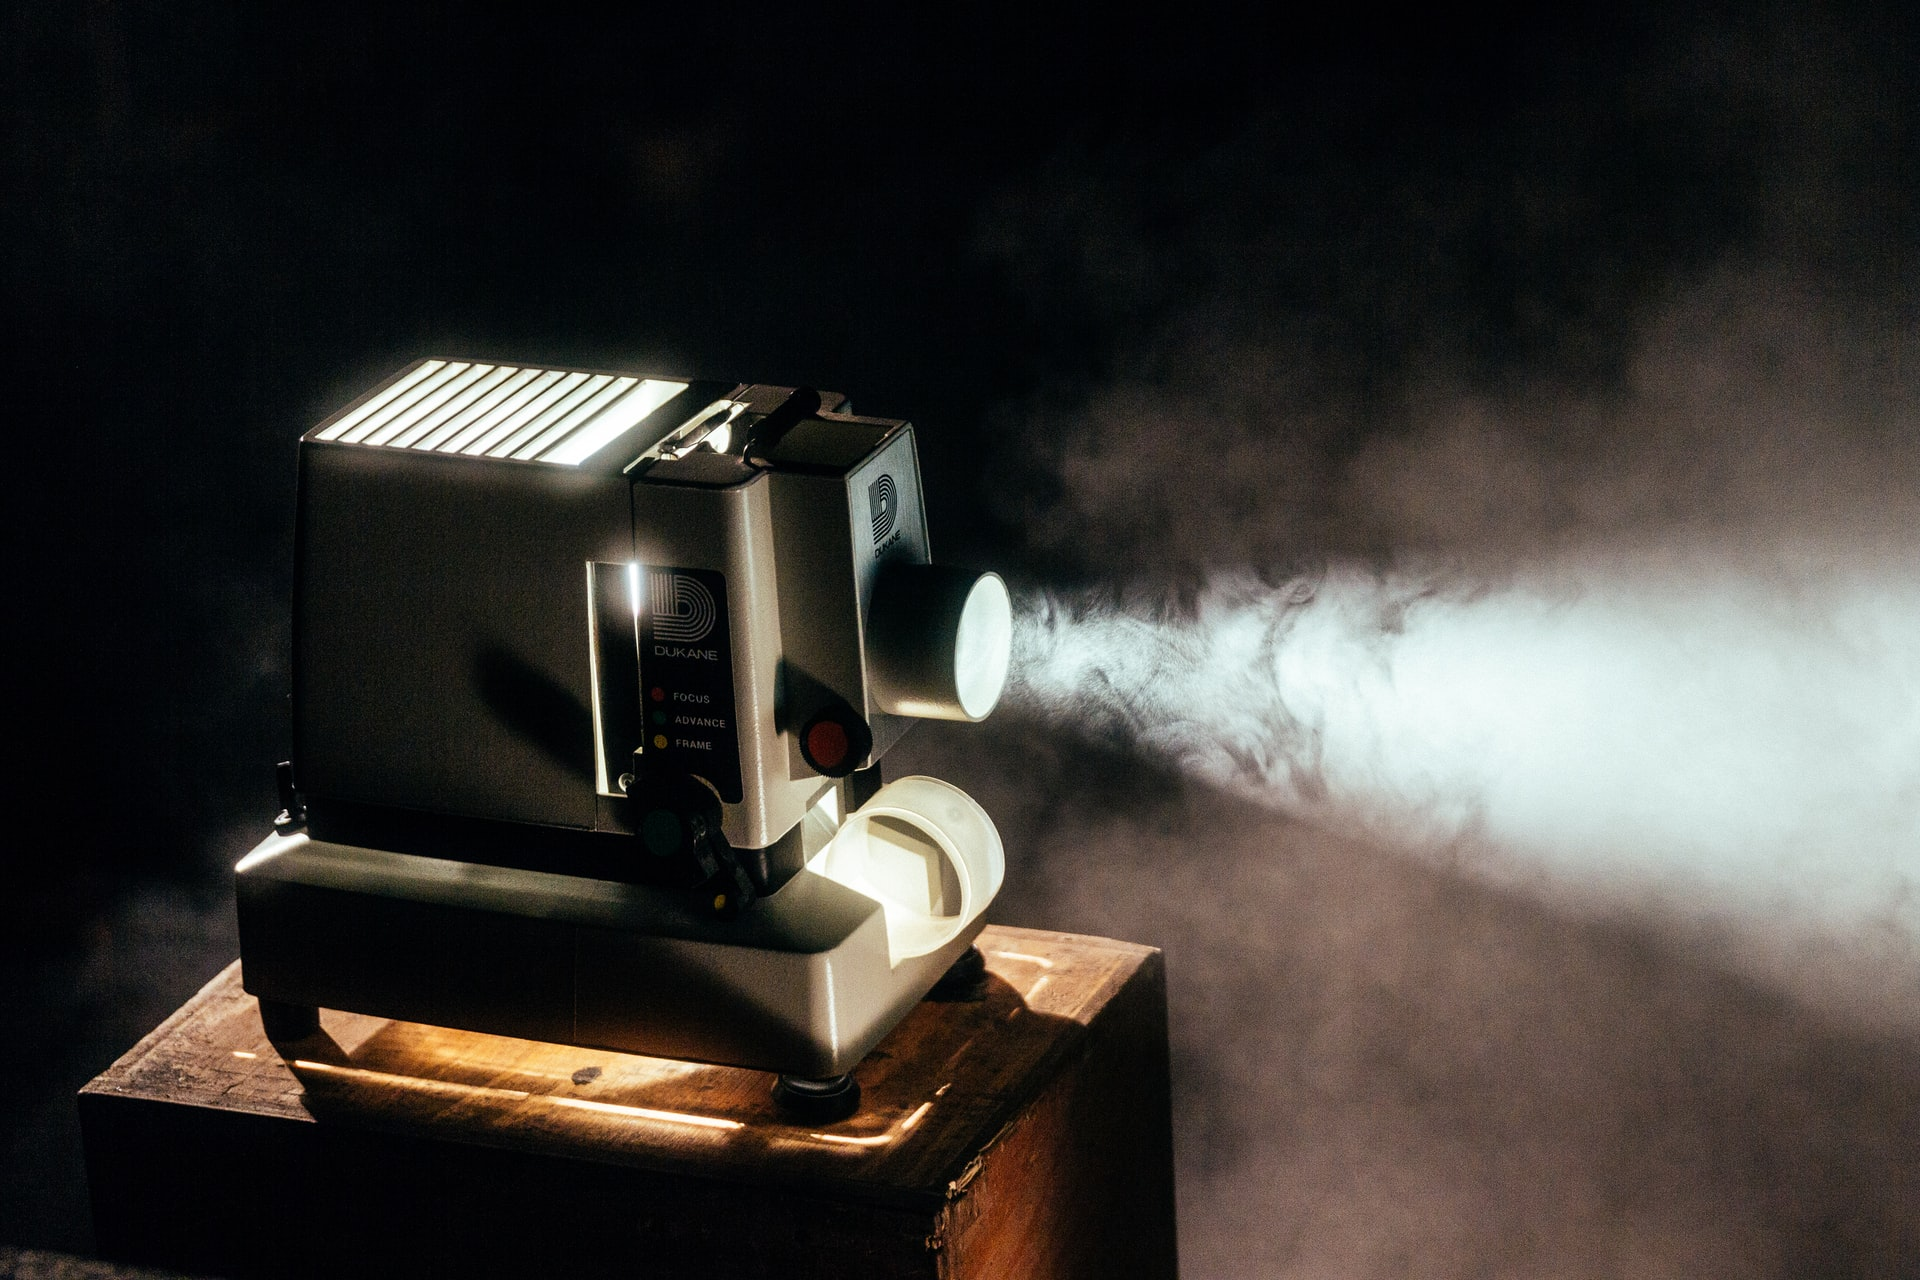
\includegraphics[width=0.8\textwidth]{images/02-projector.jpg}
    \caption{A projector is above all a light emitter. Source: \citet{ImageProjector}}
    \label{fig:background_projector}
\end{figure}

As briefly mentioned in section \ref{section:intro-problem_setting}, no projector is capable of reproducing arbitrary appearance. Each projector can only reproduce a subset of all possible colors, called the \textit{gamut}. Limited projector gamuts have a large impact on how projection mapping is done. To get a better intuition of this impact, we will now explain how a particular type of projector works. We will focus on the so-called Digital Light Processing (DLP) projector which is widely used in cinemas as well as home setups.

\subsubsection{DLP Projectors}
\label{section:background-projection_mapping-projectors-DLP}

Film projectors shine a bright light through film to project its contents onto a screen. But what happens when our movie is digital? What does a DLP projector shine its light through? And what impact does it have on its gamut?

According to \citet{WikiDLP}, DLP projectors project images by filtering the bright white light of their lamp. First, the light goes through a rapidly spinning color wheel which is split into a number of sectors: red, green, blue and sometimes also transparent. At any point, all light from the lamp passes through a single color filter, sending a single-channel image towards the lens. By sending out many single-channel images in rapid succession, however, the projector creates the illusion of sending a three-channel image.

Per-pixel intesities of this single-channel image which form its content are controlled by the Digital Micromirror Device (DMD). This device is divided into many tiny mirrors which roughly correspond to individual pixels of the projected image. Each of these mirrors can either reflect light from the color wheel directly into the lens, or into a heat sink which absorbs it and does not let it through. This allows the projector to turn pixels off and on. Grayscales (pixel intensities between full and zero) are produced by rapidly toggling the mirror between the lens and the heat sink. If, for example, a pixel is on 50\% of the time and off 50\% of the time, the resulting intensity is exactly between full and zero.

\begin{figure}[ht]
    \centering
    \begin{subfigure}[b]{0.49\textwidth}
        \centering
        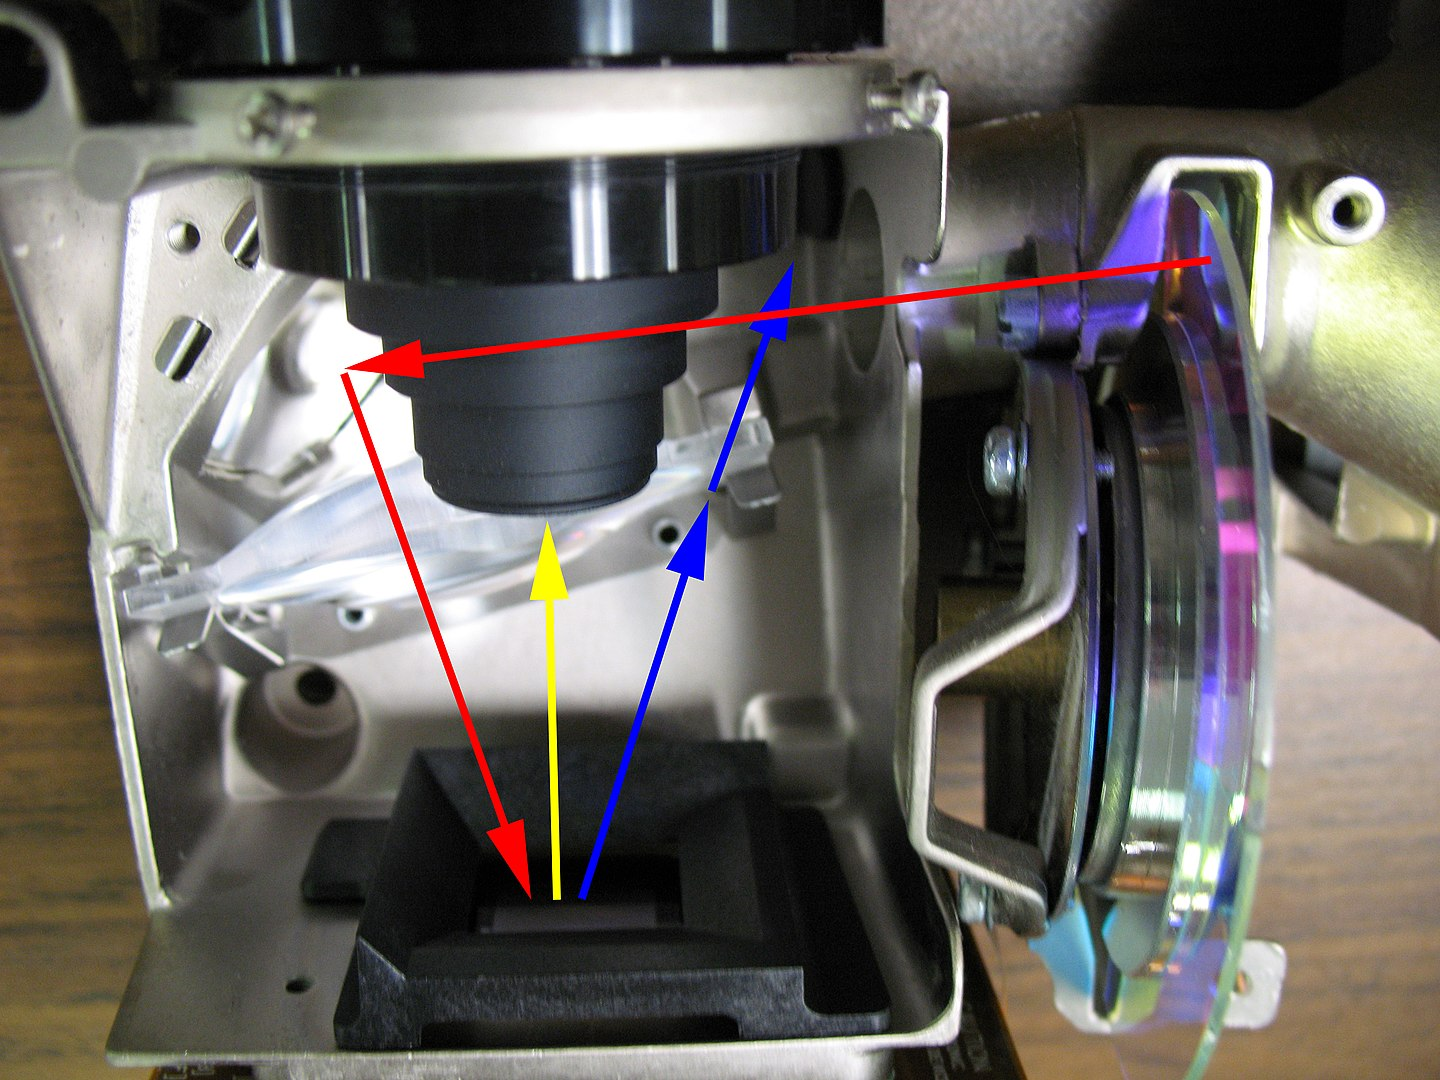
\includegraphics[width=\textwidth]{images/02-projector_dlp.jpg}
        \caption{Source: \citet{ImageProjectorDLP}}
        %\label{}
    \end{subfigure}
    \hfill
    \begin{subfigure}[b]{0.49\textwidth}
        \centering
        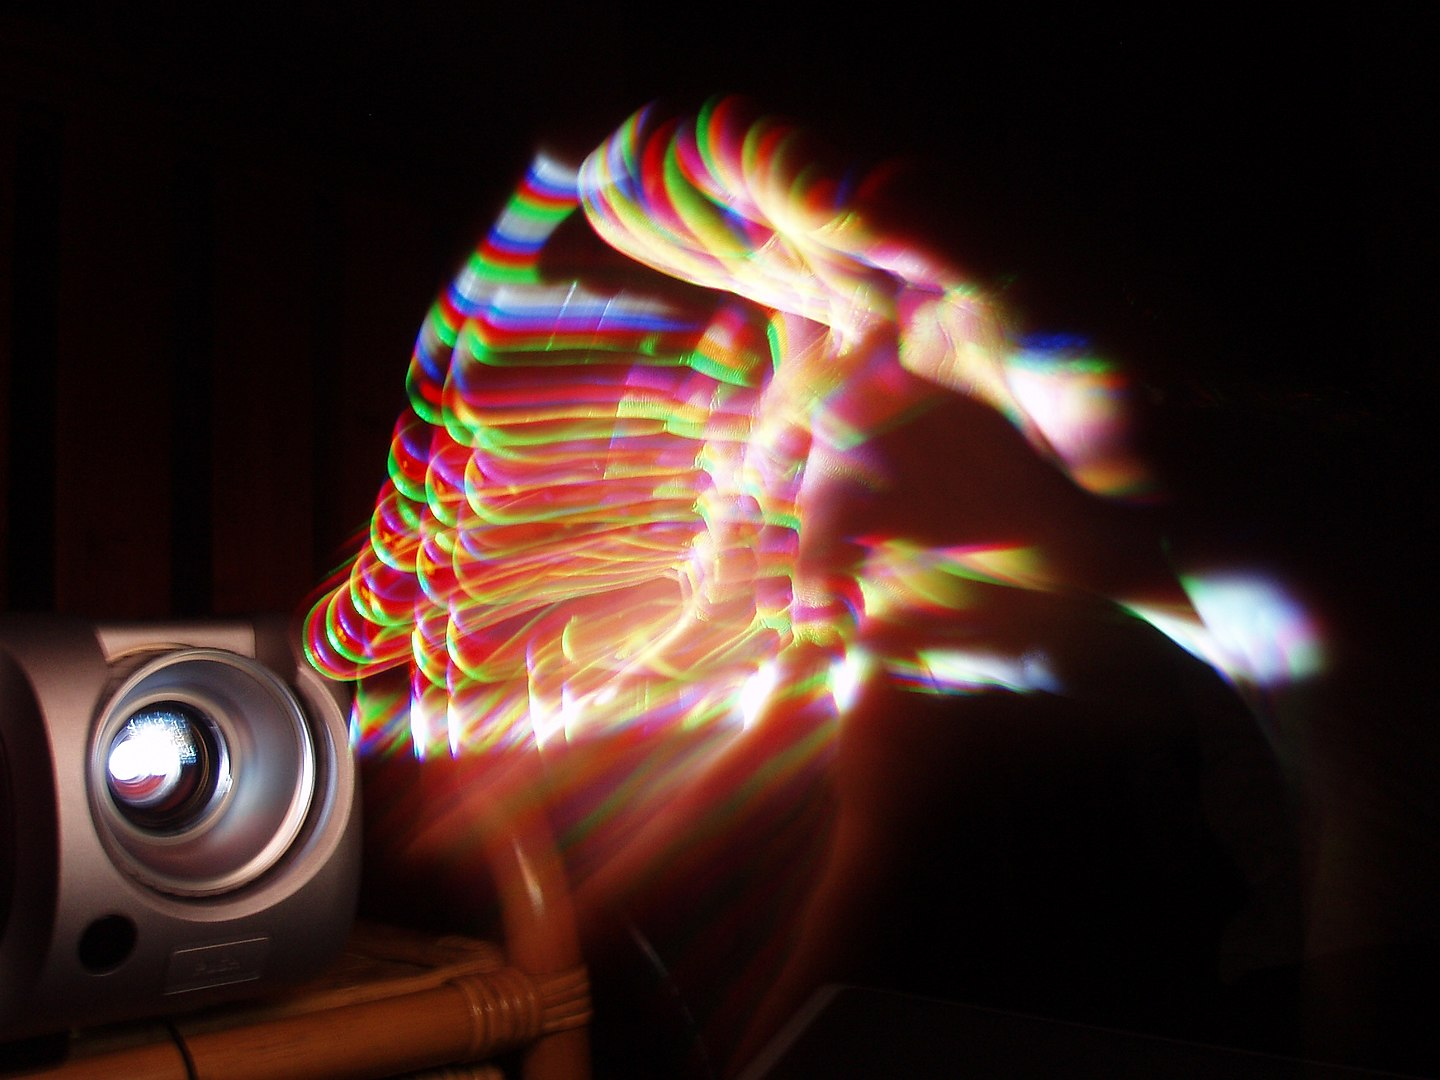
\includegraphics[width=\textwidth]{images/02-projector_rainbow.JPG}
        \caption{Source: \citet{ImageProjectorDLPRainbow}}
        %\label{}
    \end{subfigure}
    \caption{Image a) shows how a DLP projector works. First, bright white light passes through the color wheel. Then it is reflected off the the DMD (red arrows) into either the lens (yellow arrow), or the heat sink (blue arrows). Image b) shows how a DLP projector with a single DMD chip sends out single channel images in rapid succession. This can result in artifacts which can be fixed by using a separate DMD chip for each primary color}
    \label{fig:background_projector_dlp}
\end{figure}

\subsubsection{Gamut Limitations}
\label{section:background-projection_mapping-projectors-limitations}

Based on the way DLPs work, it is easy to see that the process of projecting an image is fairly inefficient since a bright white light is emitted at all times and based on the image being displayed a portion of it is sent into the heat sink and wasted. The main two limitations that result from this and that we are concerned with when projection mapping are limited maximum and minimum brightness.

Maximum brightness is simply limited by the brightness of the lamp. The brighter the lamp, the more energy it consumes and the less efficient it becomes when dark images are being projected.

Minimum brightness is related to the ability of the projector to absorb light which is not reflected directly towards the lens. The more light is absorbed inside the projector, the more the projector heats up. This is why DLP projectors with deep blacks need to be large enough to cool themselves down efficiently. If a DLP projector is not able to absorb all the light, some of it is let through towards the screen and results in dim gray instead of the intended black.

Different projector technologies have different limitations. For example, laser projectors are generally more efficient and brighter because they produce exactly the light color which is needed, as opposed to filtering out white light. But even laser projectors cannot be infinitely bright nor can they subtract light from externally illuminated scenes.

Moreover, even if a particular color lies within the gamut of our projector, the scene that we are projecting onto might prevent us from reproducing that color faithfully. The study of how light interacts with matter to influence what we see around us is called the \textit{light transport theory}. We provide a brief introduction to it in order to understand what our projections look like and which colors are and are not reproducible with a particular scene and projector. But because this theory is rather complex, we begin by building intuition on what to roughly expect when we install a projector and press Play.

{\color{red} TODO: DoF and the thin lens model? (also a limitation that's relevant for us) also pinhole!}

\subsection{Intuition on Projection Appearance}
\label{section:background-projection_mapping-projection_intuition}

The appearance of an object is given by the light it reflects. Light is the visible portion of electromagnetic radiation and consists of photons at various wavelengths. Wavelengths which human vision is sensitive to are approximately between 380 and 780 nm (\citet{PBRT3e}). Shorter wavelengths appear blue, middle ones are green and longer ones are red. Reflectance of an object is defined by the so-called \textit{spectral power distribution} (SPD) which describes what proportion of incoming light is reflected at each wavelength.

\begin{figure}[ht]
    \centering
    \begin{subfigure}[b]{0.49\textwidth}
        \centering
        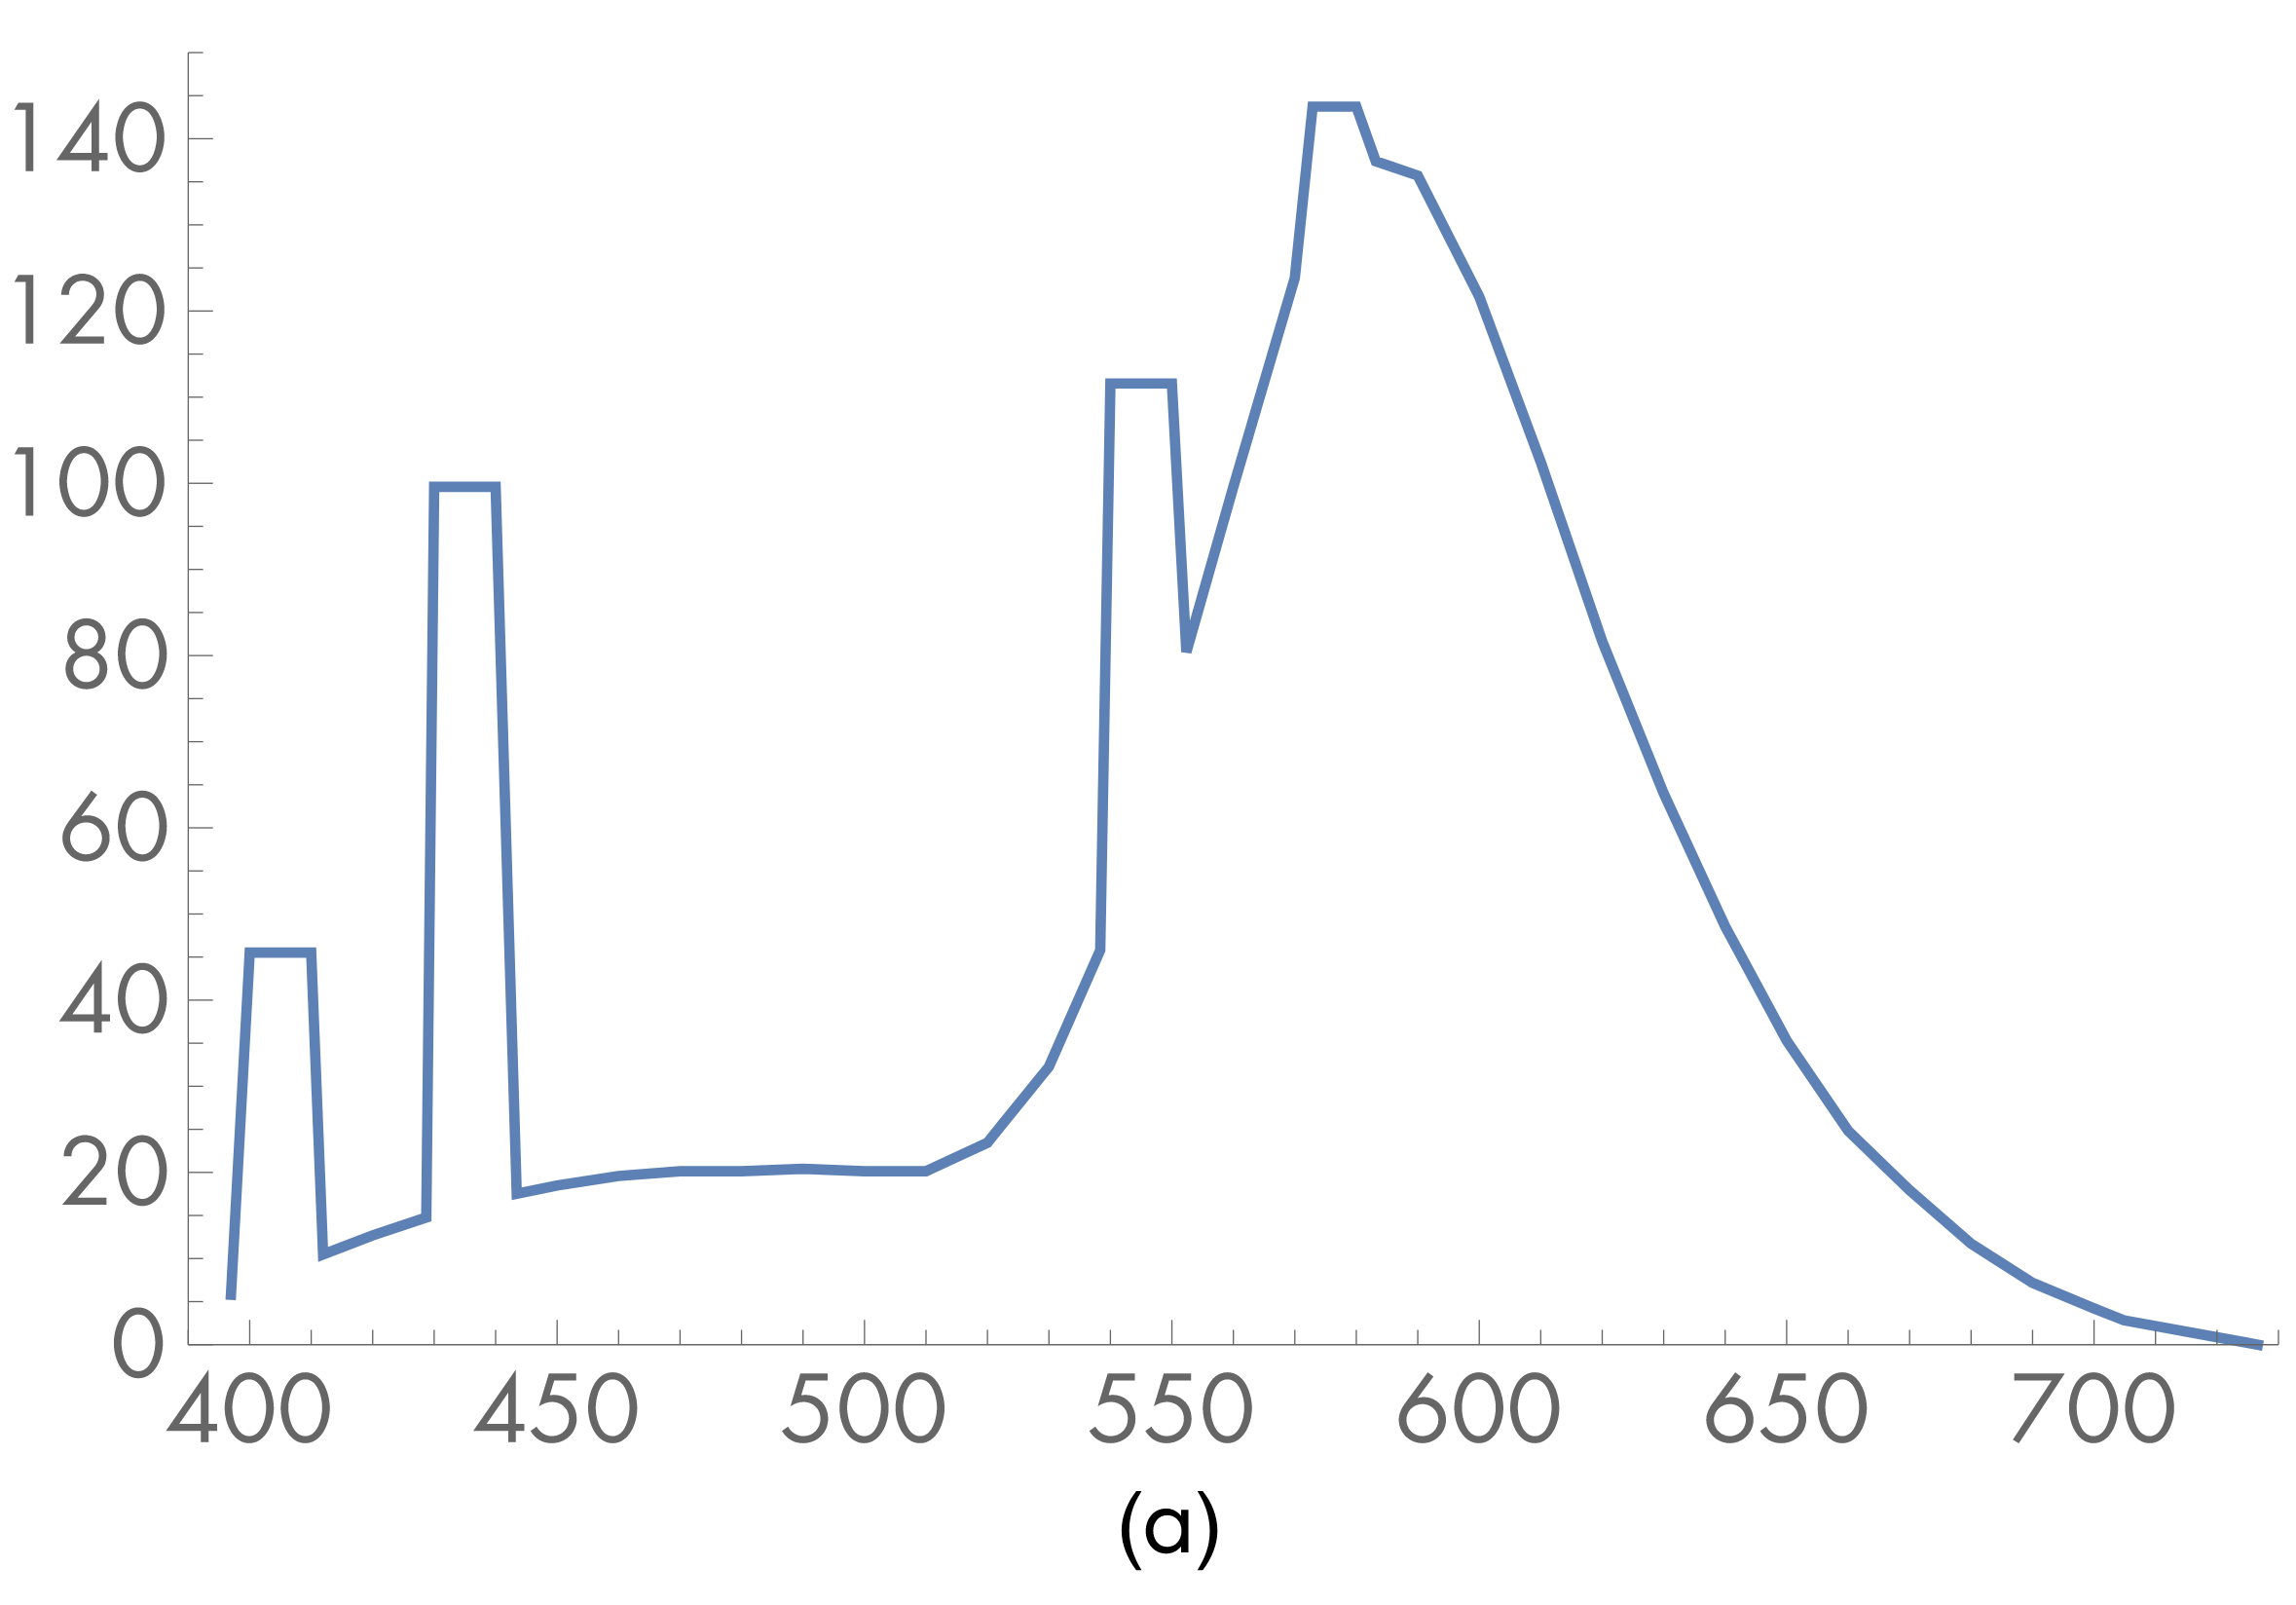
\includegraphics[width=\textwidth]{images/02-spd_fluorescent_light.png}
        \caption*{}
        %\label{}
    \end{subfigure}
    \hfill
    \begin{subfigure}[b]{0.49\textwidth}
        \centering
        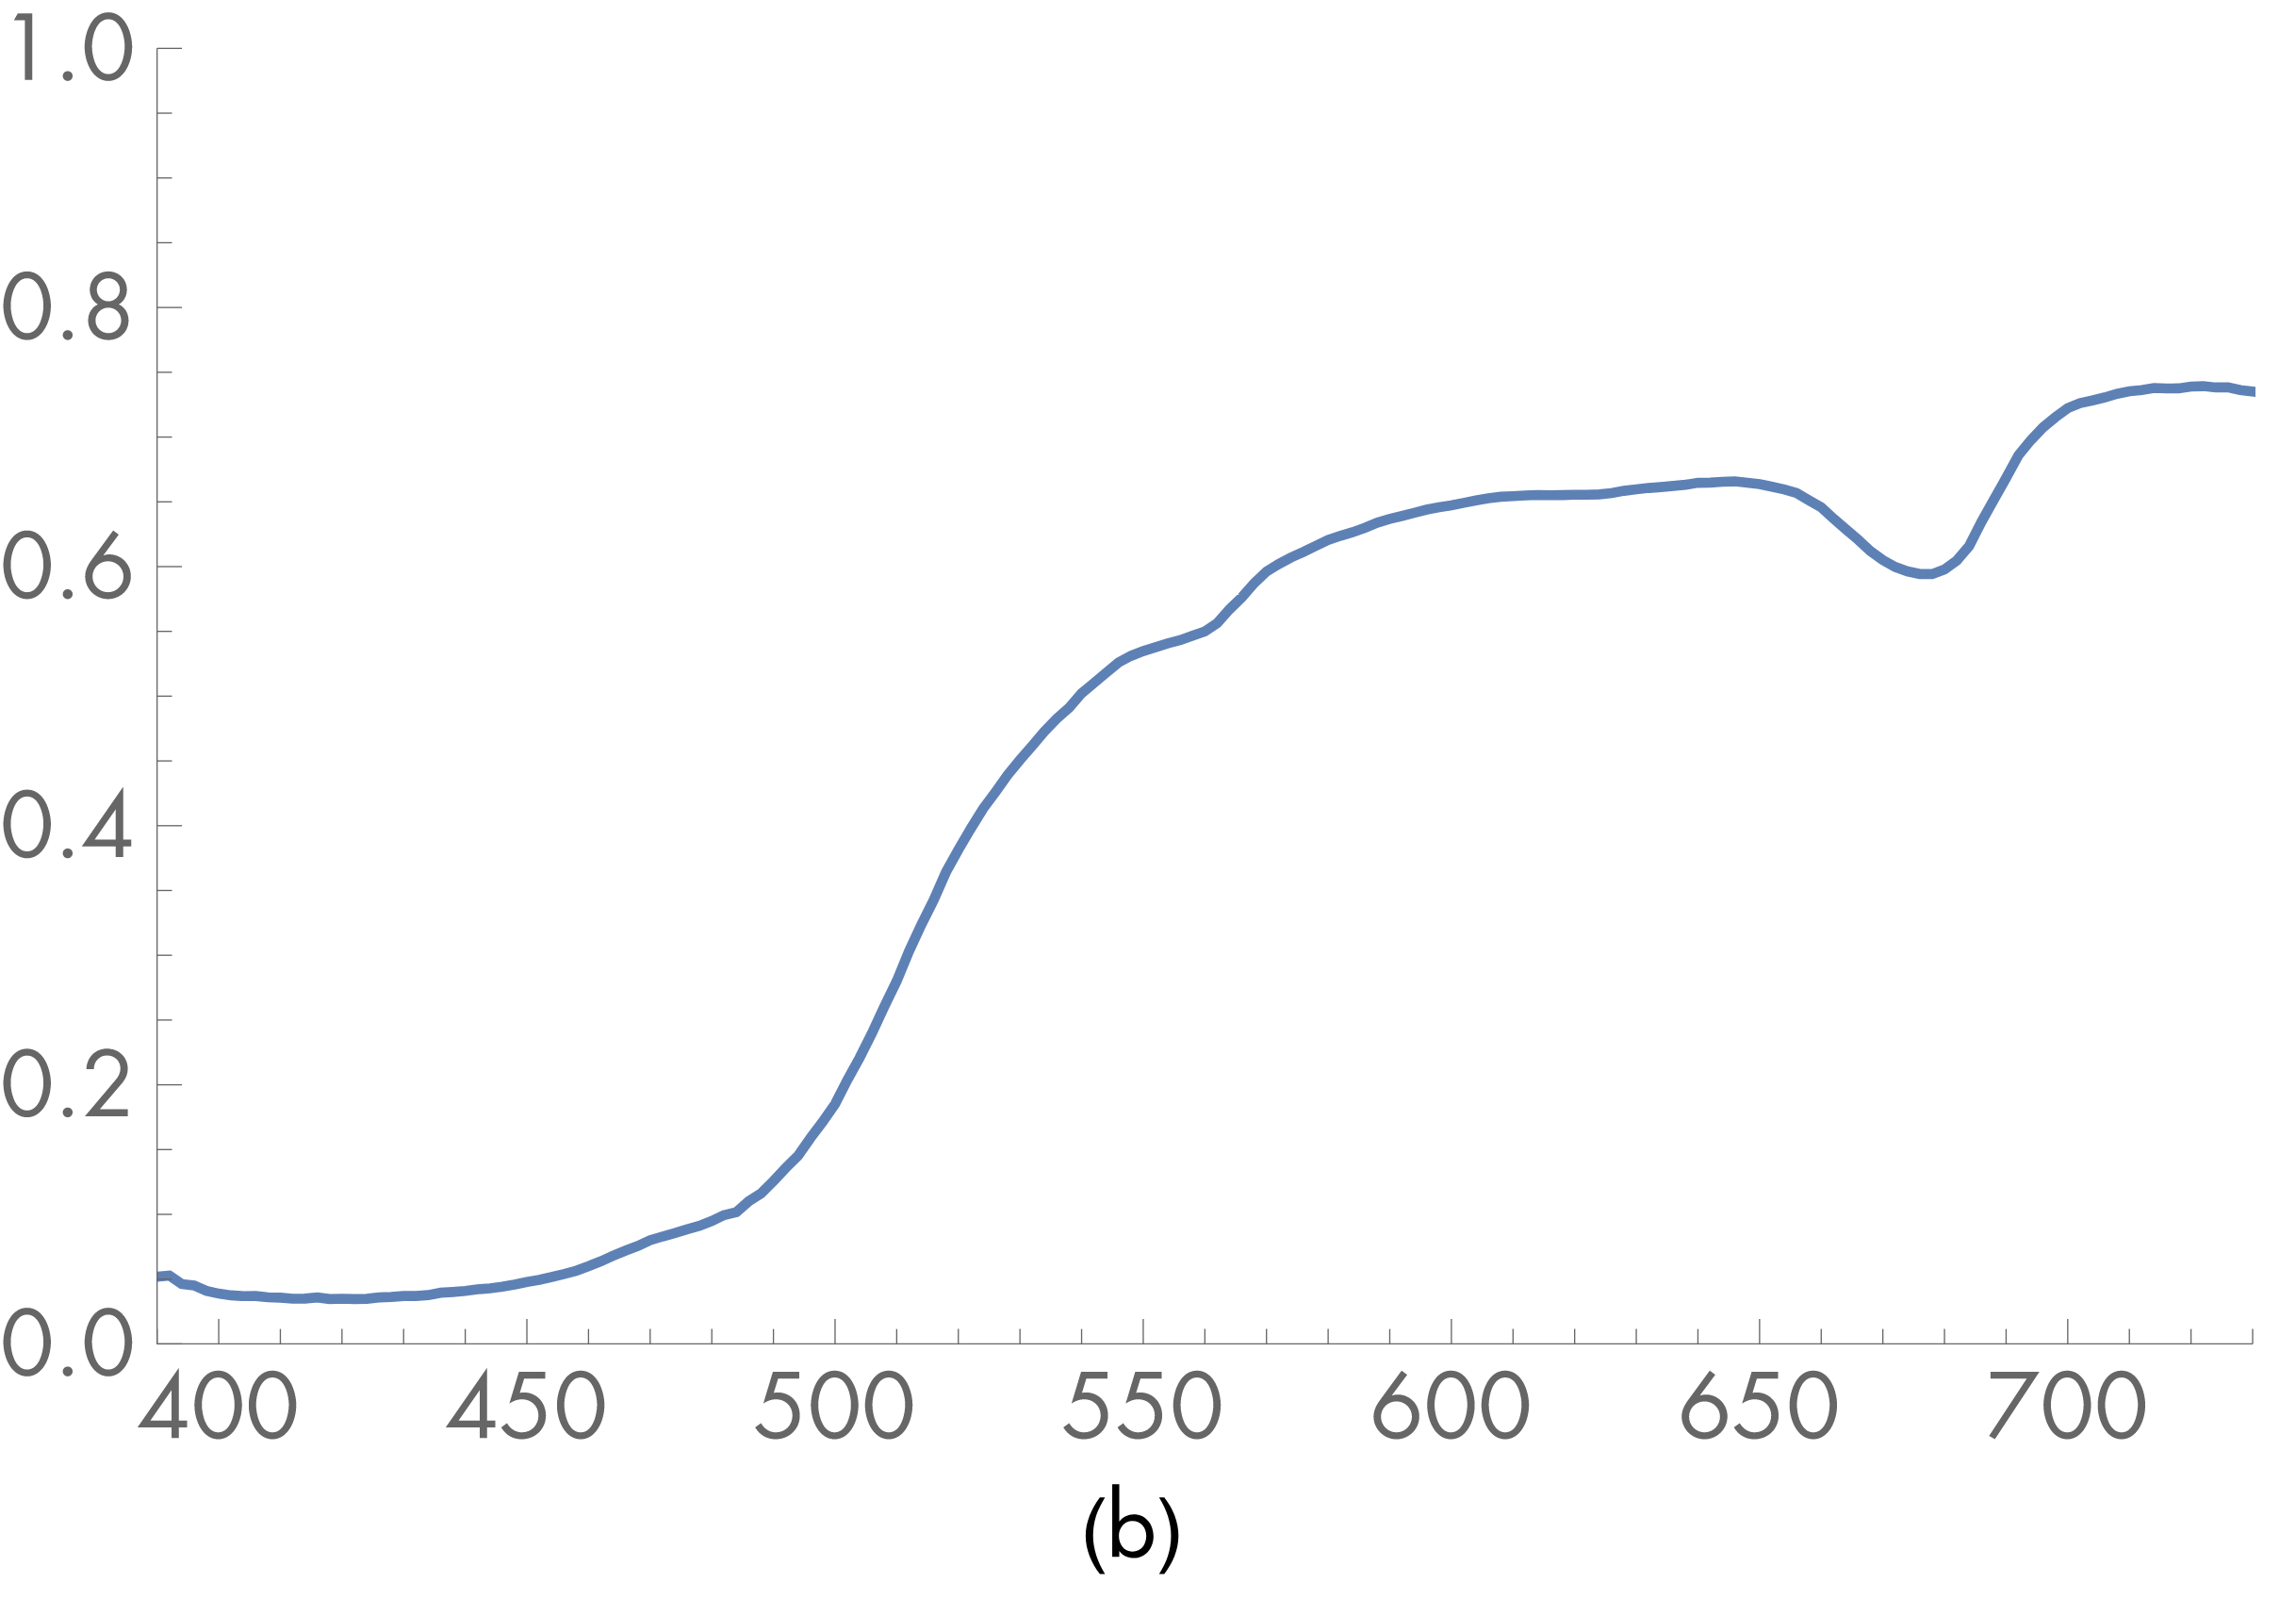
\includegraphics[width=\textwidth]{images/02-spd_lemon_peel.png}
        \caption*{}
        %\label{}
    \end{subfigure}
    \caption{Image a) shows the SPD of fluorescent light with power on the y-axis. Image b) shows the SPD of a lemon peel. Lemon peel is not an emitter hence the y-axis shows the proportion of wavelengths that are reflected off its surface. Source: \citet{PBRT3e}}
    \label{fig:background_spd}
\end{figure}

Projectors are above all light sources. As a matter of fact, each of the millions of tiny mirrors inside the DMD of a DLP projector can be thought of as a separate light source. Projector light has an SPD of its own, describing how much power it carries at each wavelength. When it interacts with a surface, something roughly corresponding to SPD multiplication takes place. If an object does not reflect any light at 450 nm, for example, all of it will be absorbed and will not reach our eyes. See fig. \ref{fig:background_spd_intuition} for examples of how projection interacts with various backgrounds.

\begin{figure}[ht]
    \centering    
    \begin{subfigure}{\textwidth}
        \centering
        \begin{subfigure}{0.24\textwidth}
            \centering
            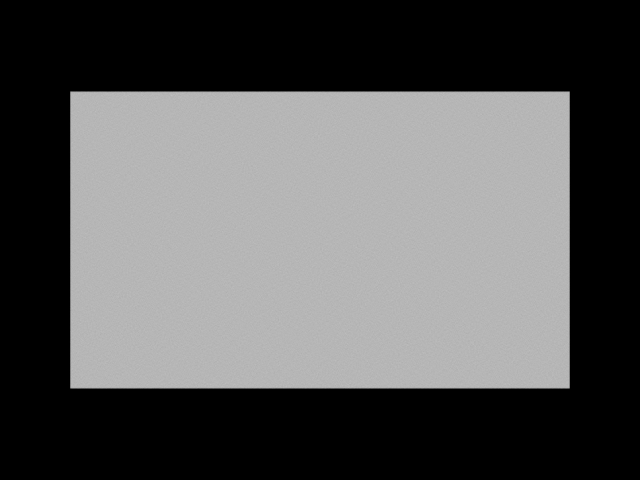
\includegraphics[width=\textwidth]{images/02-spd_intuition-white_white.png}
            \caption*{}
            \label{fig:background_spd_intuition-white_white}
        \end{subfigure}
        \hfill
        \begin{subfigure}{0.24\textwidth}
            \centering
            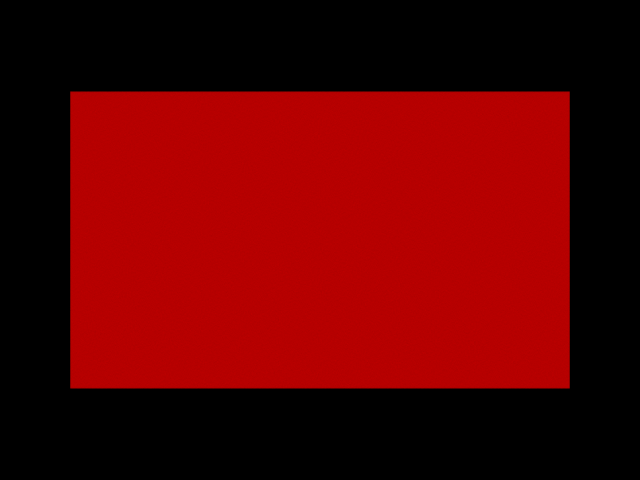
\includegraphics[width=\textwidth]{images/02-spd_intuition-white_red.png}
            \caption*{}
            \label{fig:background_spd_intuition-white_red}
        \end{subfigure}
        \hfill
        \begin{subfigure}{0.24\textwidth}
            \centering
            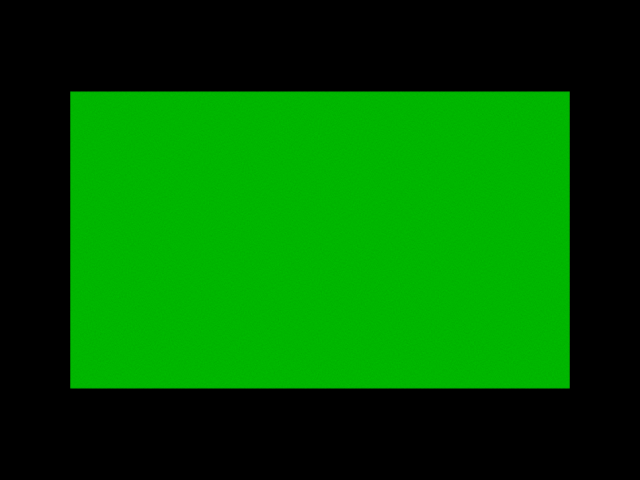
\includegraphics[width=\textwidth]{images/02-spd_intuition-white_green.png}
            \caption*{}
            \label{fig:background_spd_intuition-white_green}
        \end{subfigure}
        \hfill
        \begin{subfigure}{0.24\textwidth}
            \centering
            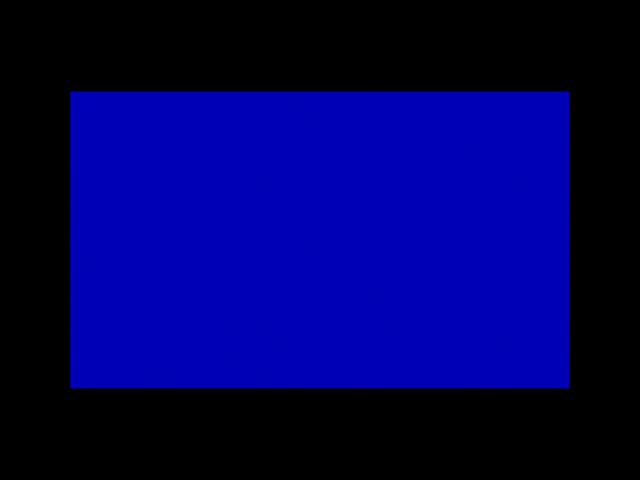
\includegraphics[width=\textwidth]{images/02-spd_intuition-white_blue.png}
            \caption*{}
            \label{fig:background_spd_intuition-white_blue}
        \end{subfigure}
        
        \begin{subfigure}{0.24\textwidth}
            \centering
            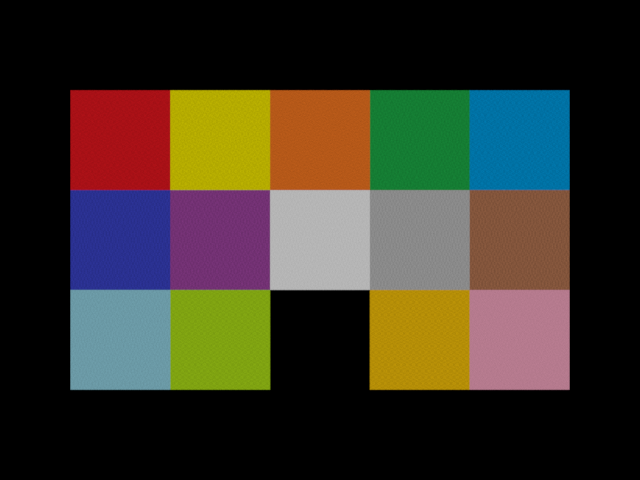
\includegraphics[width=\textwidth]{images/02-spd_intuition-palette_white.png}
            \caption*{}
            \label{fig:background_spd_intuition-palette_white}
        \end{subfigure}
        \hfill
        \begin{subfigure}{0.24\textwidth}
            \centering
            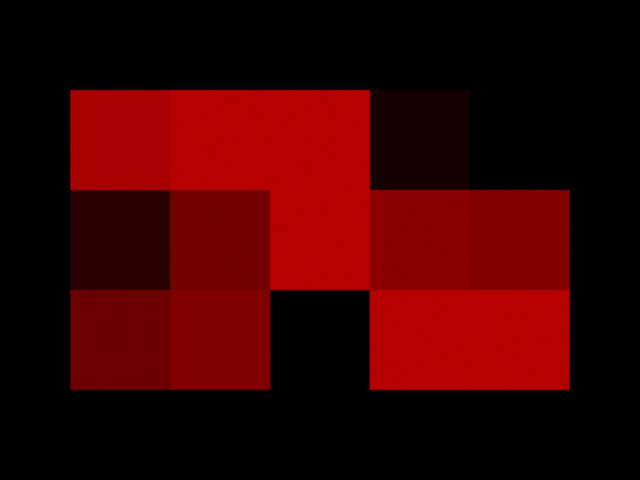
\includegraphics[width=\textwidth]{images/02-spd_intuition-palette_red.png}
            \caption*{}
            \label{fig:background_spd_intuition-palette_red}
        \end{subfigure}
        \hfill
        \begin{subfigure}{0.24\textwidth}
            \centering
            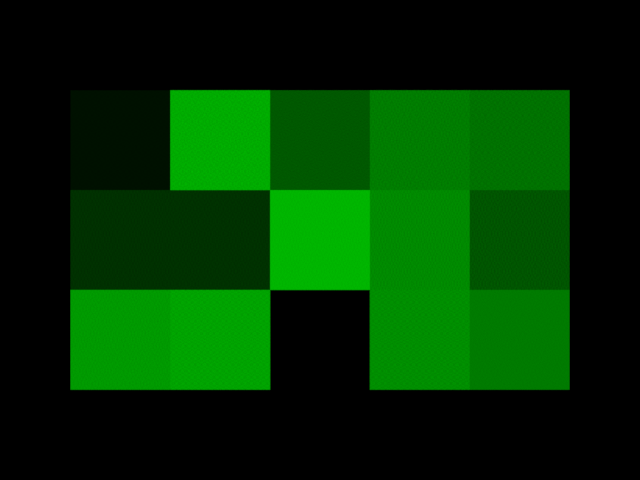
\includegraphics[width=\textwidth]{images/02-spd_intuition-palette_green.png}
            \caption*{}
            \label{fig:background_spd_intuition-palette_green}
        \end{subfigure}
        \hfill
        \begin{subfigure}{0.24\textwidth}
            \centering
            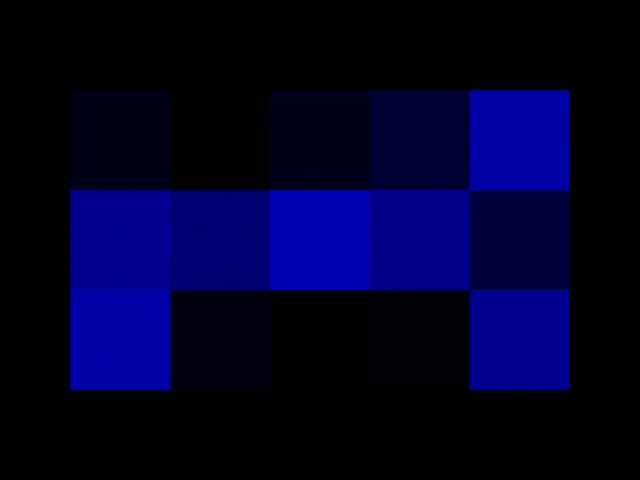
\includegraphics[width=\textwidth]{images/02-spd_intuition-palette_blue.png}
            \caption*{}
            \label{fig:background_spd_intuition-palette_blue}
        \end{subfigure}
    \end{subfigure}
    \caption{In the upper row, white light is projected onto a pure white, red, green and blue wall respectively. In the lower row, a color palette is projected onto the same backgrounds. Note that summing the last three images in each row gives the first one because each background has maximum reflectivity in one color channel and zero reflectivity in others. If a single-chip DLP projector were to project the first image, it would in fact send out the last three in rapid succession.}
    \label{fig:background_spd_intuition}
\end{figure}

We will now study this process more carefully using light transport theory.

\subsection{Light Transport Theory}
\label{section:background-projection_mapping-light_transport}

Light transport theory is the study of how light interacts with matter -- how it travels through space, scatters in fog, reflects from surfaces, refracts in camera lenses and absorbs in black T-shirts in summer. One of the most common uses of light transport is in architectural visualizations (see fig. \ref{fig:background_light_transport_examples-rendering}) and video game and movie rendering. There, we are interested in the SPD that arrives at each pixel of a virtual camera given geometry, materials and light sources.

\begin{figure}[ht]
    \centering
    \begin{subfigure}[b]{0.56\textwidth}
        \centering
        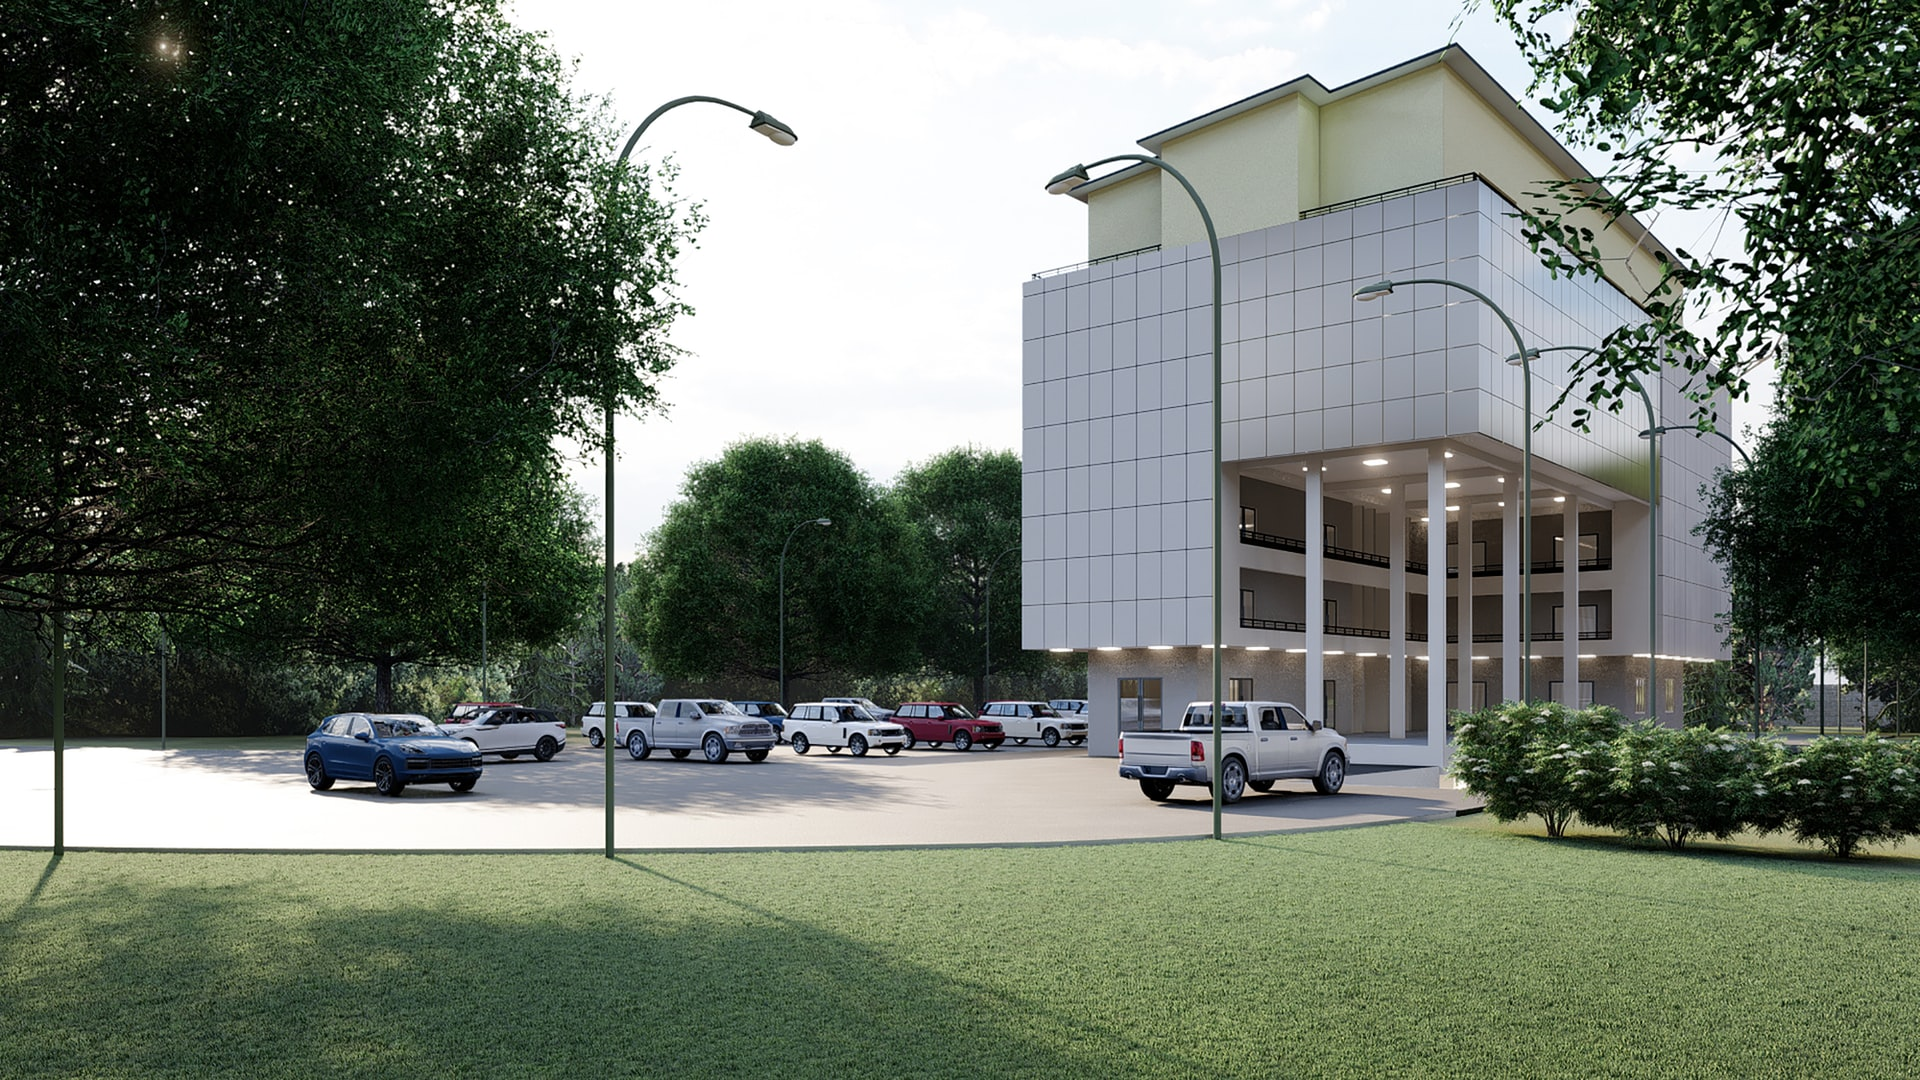
\includegraphics[width=\textwidth]{images/02-rendering.jpg}
        \caption{Source: \citet{ImageRendering}}
        \label{fig:background_light_transport_examples-rendering}
    \end{subfigure}
    \hfill
    \begin{subfigure}[b]{0.42\textwidth}
        \centering
        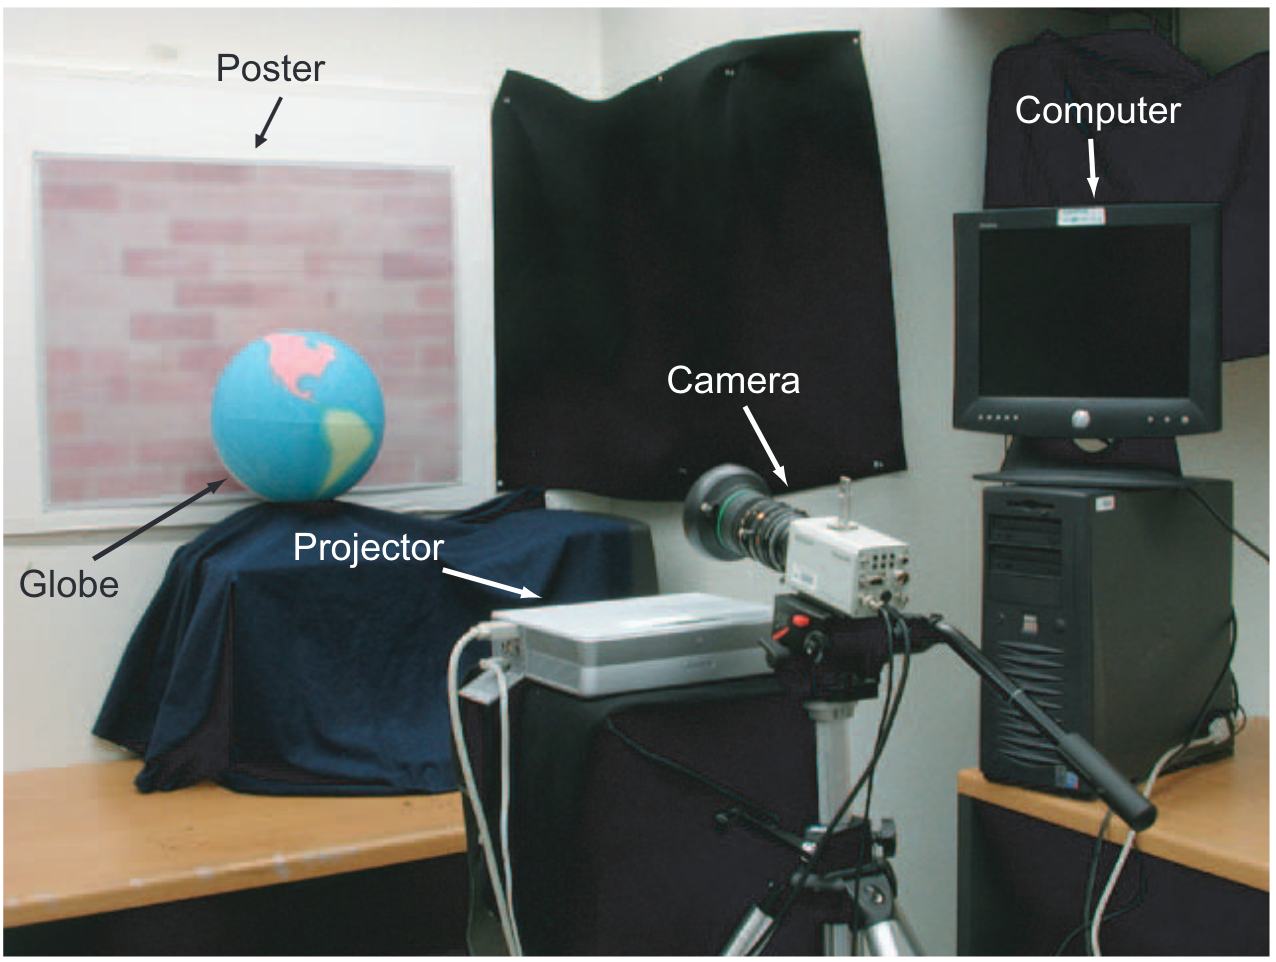
\includegraphics[width=\textwidth]{images/01-procam.png}
        \caption{Source: \citet{Grossberg2004}}
        \label{fig:background_light_transport_examples-procam}
    \end{subfigure}
    \caption{Image a) is an architectural visualization which uses light transport theory to solve the following problem: Given scene geometry, materials and light sources and camera position, what will the camera see? Image b) is a projector-camera system calibration from section \ref{section:intro-problem_setting} and asks: Given what the camera sees when various patterns are projected onto the scene, what can we say about the geometry and materials of the scene?}
    \label{fig:background_light_transport_examples}
\end{figure}

In this section, we provide a brief overview of light transport theory and explain how it can be used in projection mapping. For a more comprehensive coverage, we refer the reader to Physically Based Rendering: From Theory to Implementation by \citet{PBRT3e}.

\subsubsection{Radiance}
\label{section:background-projection_mapping-light_transport-radiance}

As mentioned in \ref{section:background-projection_mapping-projection_intuition}, all we see is light. Measuring light is therefore the crux of understanding how things look. The fundamental quantity we are interested in when measuring light is \textit{radiance}. It is defined as the amount of photons \(Q\) per unit projected area \(A^\perp \) per unit solid angle \(\omega\) per unit of time \(t\) (see fig. \ref{fig:background_radiance}):

\begin{equation}
    \label{eq:radiance}
    L = \frac{dQ}{dA^\perp d\omega dt}
\end{equation}

\begin{figure}[ht]
    \centering
    \def\svgwidth{0.8\textwidth}
    \input{images/figures/02-radiance.pdf_tex}
    \caption{Illustration of radiance which is defined as the amount of photons \(Q\) per unit projected area \(A^\perp \) per unit solid angle \(\omega\) per unit of time \(t\)}
    \label{fig:background_radiance}
\end{figure}

As suggested in fig. \ref{fig:background_spd}, to see the full picture, we need to consider radiance at each visible wavelength. A common approach to simplifying this is decompose the space of all visible SPDs into three basis functions which roughly correspond to red, green and blue colors. In that case, we would be interested in radiance in each of these channels. To simplify our explanations even further, we only talk about radiance \(L\). It is, however, important to realize that there is a layer of complexity hidden behing that notation.

Another issue with radiance is that it is a purely physical quantity while how we perceive something is to do with psychology. Luckily, for each radiometric measurement, such as radiance, there is a corresponding \(photometric\) measurement which expresses how a stimulus is perceived by the human visual system. The photometric counterpart to radiance is \(luminance\) and can be obtained from radiance by integrating against an empirically constructed spectral response curve which describes how the human eye reacts to various wavelengths. Because luminance can be easily computed from radiance, we only discuss radiance in this thesis.

We will now present the relationship between objects, light sources and the radiance incoming onto our camera sensor or eye retina. This relationship sits at the heart of light transport theory and is called the \textit{rendering equation}.

\subsubsection{Rendering Equation}
\label{section:background-projection_mapping-light_transport-rendering_equation}

The rendering equation describes the amount of outgoing radiance from point \(x\) in a scene towards a direction \(\mathbf{v}\):

\begin{equation}
    \label{eq:rendering_equation}
    L(x \rightarrow \mathbf{v}) = \int_{\Omega(x)} L(x \leftarrow \mathbf{u}) f_r(x, \mathbf{u} \rightarrow \mathbf{v}) \cos \theta d\mathbf{u} + E(x \rightarrow \mathbf{v})
\end{equation}

{\color{red} TODO: figure of rendering equation}

where \(L(x \leftarrow \mathbf{u})\) is the radiance arriving at \(x\) from direction \(\mathbf{u}\), \(\Omega(x)\) is the hemisphere oriented to the direction of the surface normal at \(x\), \(f_r\) is the spatially-varying bidirectional reflectance distribution function (SVBRDF) which determines surface reflectance for each point \(x\), incoming direction \(\mathbf{u}\) and outgoing direction \(\mathbf{v}\), and \(\theta\) is the angle between \(u\) and the surface normal at \(x\). Finally, \(E(x \rightarrow \mathbf{v})\) is the radiance emitted from \(x\) towards \(\mathbf{v}\) in case \(x\) lies on a light source.

The main idea of the equation is that radiance leaving towards \(\mathbf{v}\) from \(x\) is the sum of reflected and emitted radiance. It assumes empty space between objects, therefore no light scattering occurs between them. This means that radiance is constant along straight lines and the equation is recursive -- \(L(x \leftarrow \mathbf{u}) = L(y \rightarrow -\mathbf{u})\) where \(y\) is the point seen from \(x\) in the direction of \(\mathbf{u}\). Generalizations of the rendering equation to scenes with participating media where this is not the case are discussed in a SIGGRAPH course by \citet{Novak2018}.

Apart from assuming that our objects are in vacuum, the equation also assumes that light is reflected from the same point it arrived at. This is generally not the case as can be seen for example with human skin where light bounces under the surface before it is reflected. This phenomenon is known as \textit{subsurface scattering} and a generalization of the rendering equation to account for it has been presented for example by \citet{Jensen2001}. For our purposes, however, it is sufficient to be familiar with the basic form of the rendering equation.

To determine the amount of radiance that hits a virtual camera sensor in scenes such as fig. \ref{fig:background_light_transport_examples-rendering}, we need to solve the rendering equation for points that lie on the sensor and directions towards points in the scene that are visible from the sensor. This is typically done by Monte Carlo integration which estimates the integral by random sampling. Each sample is a light path from a light source towards the camera with zero or more bounces on the surfaces of the scene. A strategy to choose such samples is crucial to the performance of a rendering algorithm. A brilliant overview of sampling strategies, for example bidirectional path tracing (BDPT) can be found in \citet{Veach1997}.

\subsubsection{Towards Projection Mapping}
\label{section:background-projection_mapping-light_transport-towards_projection_mapping}

In a sense, projection mapping is a more difficult problem than rendering. Whereas in rendering, the scene geometry, materials and light sources are known and the radiance at the camera sensor is unknown, in projection mapping we only know the radiance at the camera sensor and everything else, including the projection image (our light source), is unknown.

{\color{red} TODO: figure that compares rendering to projection mapping}

Projection mapping algorithms therefore do not typically solve the full (inverse) light transport of the whole scene, but instead they build on top of assumptions and provide estimates. Common assumptions are for example

\begin{itemize}
    \item A known relationship between the projector and camera orientation
    \item Absence of glossy surfaces whose appearance depends on view point
    \item A 1:1 correspondence between projector and camera pixels, meaning that each pixel of the camera image is influenced by only one projector pixel. Note that this does not hold for example in scenes with convex geometry where light from multiple projector pixels is concentrated into a single camera pixel
\end{itemize}

We will now review some common approaches to projection mapping found in state-of-the-art methods. Our goal is to use this information to construct a reference method that we can implement in our projector-camera system simulator and use in experiments to compare our proposed projection mapping method against.

\subsection{Projector-Camera Systems}
\label{section:background-projection_mapping-procams}

The key idea in projection mapping is to use a camera to observe the projection and provide information on how to adapt it to achieve desired appearance. This system as a whole is called the \textit{projector-camera system}, commonly shortened as \textit{procam}.

As mentioned in eq. \ref{eq:projection_mapping-per_pixel}, this adaptation is done by modifying the projector image until the camera image matches the desired appearance pixel by pixel. However, the relationship between projector and camera pixels is very complex, as suggested in section \ref{section:background-projection_mapping-light_transport} on light transport theory. The model of this relationship is the main differentiating factor of various projection mapping methods.

On a high level, projection mapping methods can be split into two groups:

\begin{itemize}
    \item Those that assume a 1:1 correspondence between projector and camera pixels
    \item Those that do not and instead attempt to solve general light transport in the whole scene
\end{itemize}

The first group usually has two smaller tasks to perform. First, they need to establish those correspondencies geometrically in a step called \textit{geometric calibration}. Then, they need to model how the intensity of a projector pixel affects the intensity of the corresponding camera pixel in a step called \textit{radiometric calibration}. Despite the original assumption of 1:1 pixel correspondence, these methods are reasonably general and work quite well. They are also the most common. We will therefore review a few of them and focus on how projector hardware (along with scene complexity) limits their performance.

The second group typically uses \textit{inverse light transport} to model the relationship between projector and camera as generally as possible. These methods are mostly limited by the computational complexity of such a task. Some, for example \citet{Siegl2017}, achieve real time performance at the cost of using an additional depth camera to gain more information about the scene and projecting only on matte objects of constant color. We will focus on an older method by \citet{Wetzstein2007} that works with arbitrarily complex scenes and will thus be useful for us when constructing our reference method.

For a complete overview of the state of the art in projection mapping, see \citet{Grundhofer2018}.

\subsubsection{Geometric Calibration}
\label{section:background-projection_mapping-procams-geometric_calibration}

The goal of geometric calibration is to find a point \(M_c = [u_c, v_c]^T\) in the camera image for each point \(M_p = [u_p, v_p]^T\) in the projector image such that the value of the latter determines the value of the former. These correspondencies are usually established via a third point, \(P = [x, y, z]\) which is located in the scene.

The relationship between \(M_c\) and \(P\) is determined by the \textit{intrinsic} and \textit{extrinsic} matrices:

\begin{equation}
    \label{eq:camera_equation}
    \begin{bmatrix}
        u_c \\
        v_c \\
        1
    \end{bmatrix} =
    \begin{bmatrix}
        f_x & s & u \\
        0 & f_y & v \\
        0 & 0 & 1 
    \end{bmatrix} \cdot
    \begin{bmatrix}
        \mathbf{R} & \mathbf{t}
    \end{bmatrix} \cdot
    \begin{bmatrix}
        x \\
        y \\
        z
    \end{bmatrix}
\end{equation}

where the intrinsic matrix is formed by camera focal lengths \(f_x\) and \(f_y\) (focal length is expressed in pixels and if pixels are square, then \(f_x = f_y = f\)), skewness \(s\) of image axes, and principal point coordinates \([u, v]^T\) (the intersection of optical axis and image plane which is generally not in the center of the image). The extrinsic matrix is then formed by rotation \(\mathbf{R}\) and translation \(\mathbf{t}\) which convert between world coordinates and camera coordinates. See fig. \ref{fig:background_camera_calibration} for an illustration.

\begin{figure}[ht]
    \centering
    \def\svgwidth{0.8\textwidth}
    \input{images/figures/02-camera_calibration.pdf_tex}
    \caption{Illustration of geometric calibration of projector and camera. Points \(M_c\) and \(M_p\) on camera and projector image plane, respectively, are related via a point \(P\) in the scene. \(f\) is the focal length which is the distance between pinhole and principle point and \(u\) and \(v\) are principle point coordinates with respect to image plane origin}
    \label{fig:background_camera_calibration}
\end{figure}

The most commonly used method for finding the parameters of eq. \ref{eq:camera_equation} was introduced by \citet{Zhang1999}. They are estimated by taking at least two photos of a planar pattern at various orientations.

We will now outline two recent methods to perform geometric calibration. The first one requires user assistance, while the second one is fully automatic.

\textbf{One camera, one projector and a calibration board.} The first method, introduced by \citet{Yang2016}, uses a calibration board containing a random dot pattern. First, the camera is calibrated using the approach of \citet{Zhang1999}. Then the projector is calibrated by projecting another dot pattern onto the board and treating the projector as an inverse camera. The whole process needs around 10 views of the calibration board according to experiments in the paper.

\textbf{Two cameras, one projector.} An entirely automatic self-calibration method was presented by \citet{Willi2017}. Their method first establishes pixel correspondencies between the two cameras and then continues to estimate the intrinsic and extrinsic matrix, as well as the 3D point cloud of the scene. Finally, the projector is calibrated using this information. It is worth noting that this method works also for any larger number of projectors and cameras in which case camera pairs are sorted by the quality of their pixel correspondencies. Calibration is first done for the best pair and other devices are incorporated iteratively, improving the overall estimate.

\subsubsection{Radiometric Calibration}
\label{section:background-projection_mapping-procams-radiometric_calibration}

Once correspondencies between projector and camera pixels have been established, radiometric calibration can be performed. In general, the goal is to find a color-mapping function \(f\) such that

\begin{equation}
    \label{eq:radiometric_calibration}
    \begin{bmatrix}
        C_R \\
        C_G \\
        C_B
    \end{bmatrix} = f(
        \begin{bmatrix}
            P_R \\
            P_G \\
            P_B
        \end{bmatrix}
    )
\end{equation}

where \(C\) is the color of a camera pixel and \(P\) is the color of the corresponding projector pixel. We describe one method that assumes \(f\) to be linear and one method that allows for arbitrary \(f\).

\textbf{Linear color-mapping function.} One of the first projection mapping methods was presented by \citet{Grossberg2004}. There, the relationship between \(c_c\) and \(c_p\) is specified as follows:

\begin{equation}
    \label{eq:linear_color_mapping}
    \begin{bmatrix}
        C_R \\
        C_G \\
        C_B
    \end{bmatrix} = p_c(
        \begin{bmatrix}
            V_{RR} & V_{RG} & V_{RB} \\
            V_{GR} & V_{GG} & V_{GB} \\
            V_{BR} & V_{BG} & V_{BB}
        \end{bmatrix} \cdot p_p(
            \begin{bmatrix}
                P_R \\
                P_G \\
                P_B
            \end{bmatrix}
        ) +
        \begin{bmatrix}
            F_R \\
            F_G \\
            F_B
        \end{bmatrix}
    )
\end{equation}

where \(p_p\) is a non-linear projector response function which turns input pixel values into projector brightness, \(p_c\) is a non-linear camera response that converts radiance arriving at the camera sensor to output pixel value, \(F = [F_R, F_G, F_B]^T\) is the environment light term which is independent of the projector, and finally \(V\) is a \(3 \times 3\) color mixing matrix which captures the relationship between projector and camera channels and their interactions with spectral reflectance.

Both \(p_p\) and \(p_c\) are independent of the scene and can be estimated separately. \(V\) and \(F\) are per-pixel and scene-dependent and can be estimated by projecting and capturing 6 calibration images.

The disadvantage of this method is that the linear color mixing matrix is not an accurate model for example when using DLP projectors described in section \ref{section:background-projection_mapping-projectors-DLP}. DLP projectors sometimes form an image by composing red, green, blue and white channels together. The extra white channel may result in non-linear behavior. Another disadvantage is related to projector brightness limitations. If the color gamut of the projector struggles to reproduce the color required by the compensation model, it results in clipping artifacts and lowered contrast. See fig. \ref{fig:background_clipping} for an illustration.

\begin{figure}[ht]
    \centering
    \def\svgwidth{0.6\textwidth}
    \input{images/figures/02-clipping.pdf_tex}
    \caption{Illustration of reduced contrast due to brightness limitations. Projector gamut is delimited by a triangle. If a compensation model requires a color which is outside the triangle, the closes color on the edge of the triangle is projected instead. Colors inside the triangle are projected as required which results in reduced contrast between the two groups}
    \label{fig:background_clipping}
\end{figure}

\textbf{Non-linear color-mapping function with a global optimization step.} To solve these problems, \citet{Grundhofer2015} presented an improved method which allows for an arbitrary color-mixing function. This function is estimated by obtaining up to \(6^3\) samples and then applying thin-plate spline interpolation on them. This sampling process takes several minutes but once it is completed, compensation can be performed in real time.

Moreover, the paper acknowledges that the contrast issues stem from the way the camera image is matched with the desired appearance pixel by pixel (see eq. \ref{eq:projection_mapping-per_pixel}). To fix this, it uses a global optimization step which compensates the image based on its higher level content. In this step, a patch size is chosen (typically \(2^n\) pixels) and a color-correcting coefficient is introduced for each patch. The coefficients are set so as to minimize clipping errors caused by limited color gamut of the projector and overall increase image contrast.

\begin{figure}[ht]
    \centering
    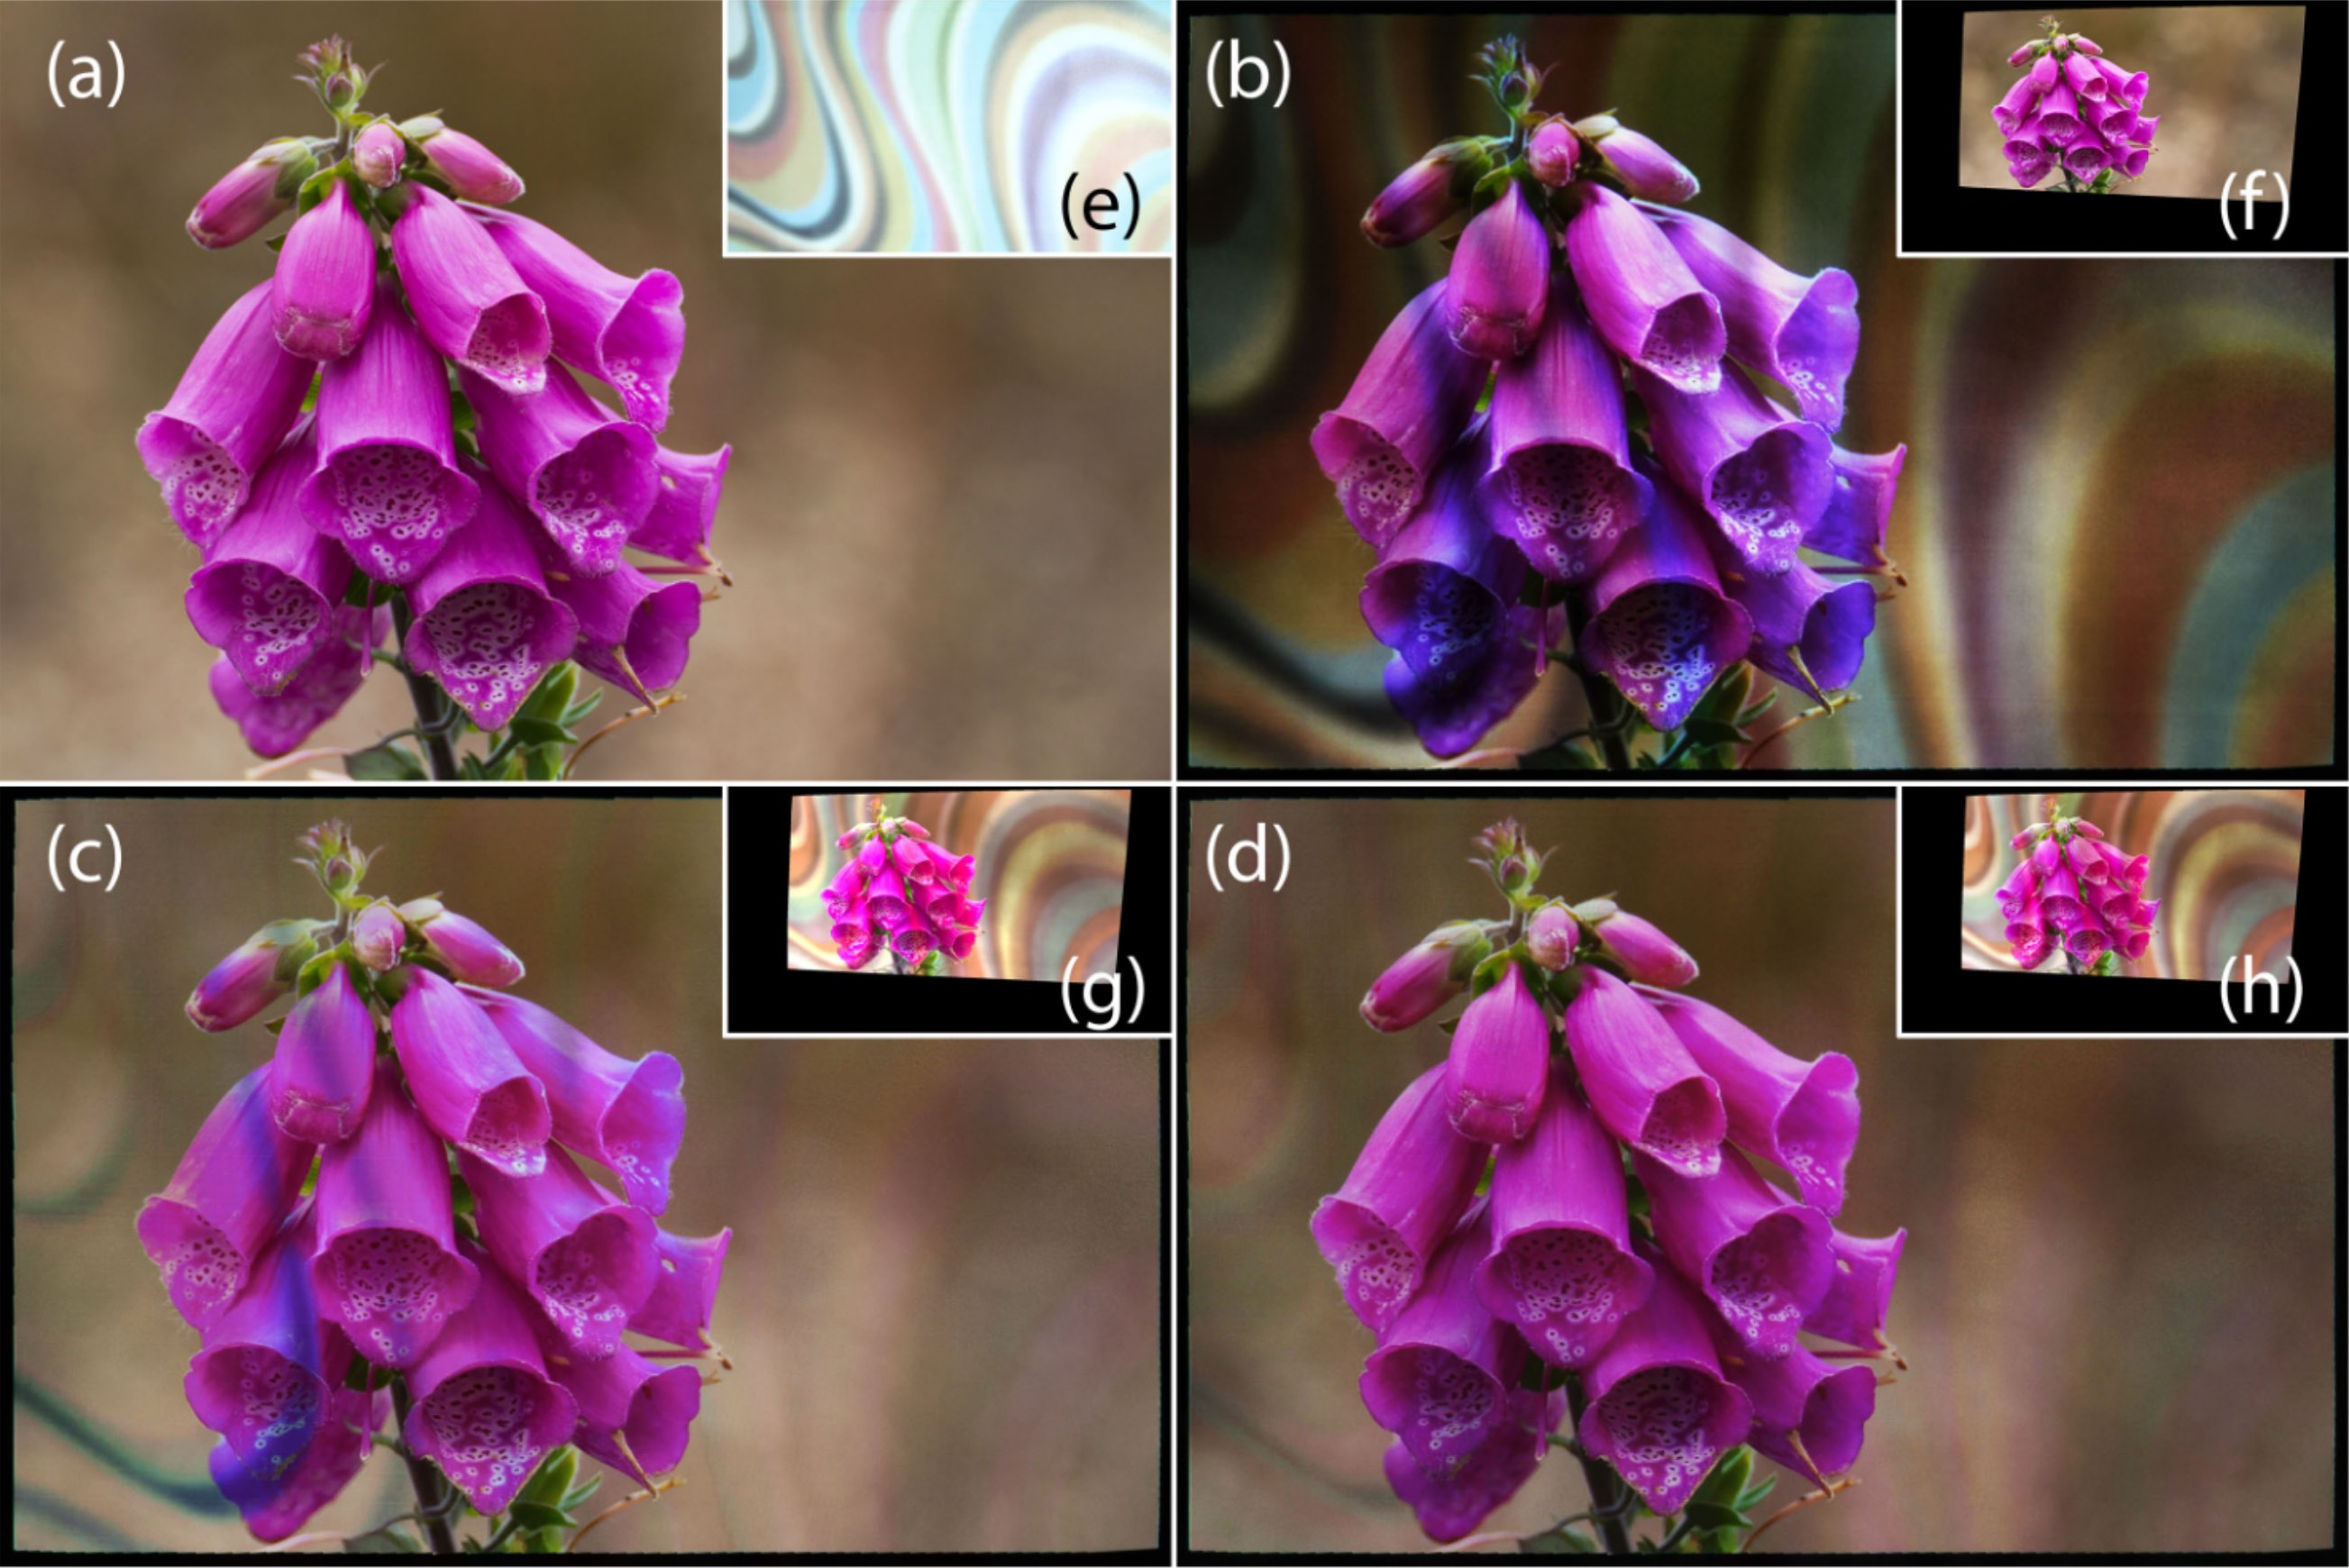
\includegraphics[width=0.6\textwidth]{images/02-grundhofer_result_compressed.jpg}
    \caption{Results of a projection mapping method by \citet{Grundhofer2015}. (a) original input image. (e) non-uniformly colored projection surface (illuminated  uniformly white). (b) captured projection of (a) on (e). (c) captured  projected  compensation  image shows local clipping errors. (d) reduced clipping errors after applying a global optimization step. (f-h) geometrically warped projection images generating camera images (b-d). Source: \citet{Grundhofer2015}}
    \label{fig:background_grundhofer_result}
\end{figure}

As a result, this method achieves very good results in scenes which have minimal inter-reflection that cannot be modeled when 1:1 correspondence between projector and camera pixels is assumed (see fig. \ref{fig:background_grundhofer_result}). The idea of the global optimization step is important because goes in the same direction as our method -- compensating the projection image not pixel by pixel, but based on higher-level content instead.

\subsubsection{Inverse Light Transport}
\label{section:background-projection_mapping-procams-inverse_lt}

Another approach to projection mapping that does not rely on the assumption of 1:1 correspondence between projector and camera pixels is so-called inverse light transport. The basic idea behind this approach is that radiance incoming onto camera sensor is a linear function of light sources in the scene. This can be derived directly from the rendering equation (see eq. \ref{eq:rendering_equation}) and practical examples can be seen in fig. \ref{fig:background_linear_lt}.

\begin{figure}[ht]
    \centering
    \begin{subfigure}[b]{0.24\textwidth}
        \centering
        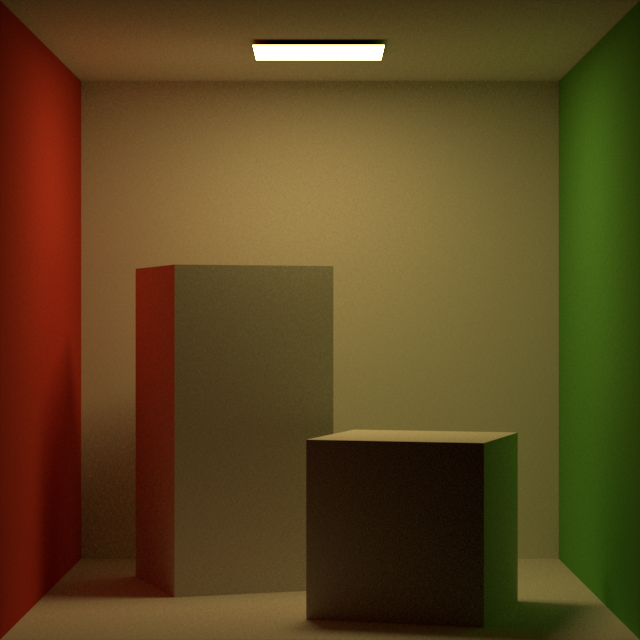
\includegraphics[width=\textwidth]{images/02-linear_lt_light01.jpg}
        \caption*{\(a = 1.0\), \(b = 0.0\)}
        %\label{}
    \end{subfigure}
    \hfill
    \begin{subfigure}[b]{0.24\textwidth}
        \centering
        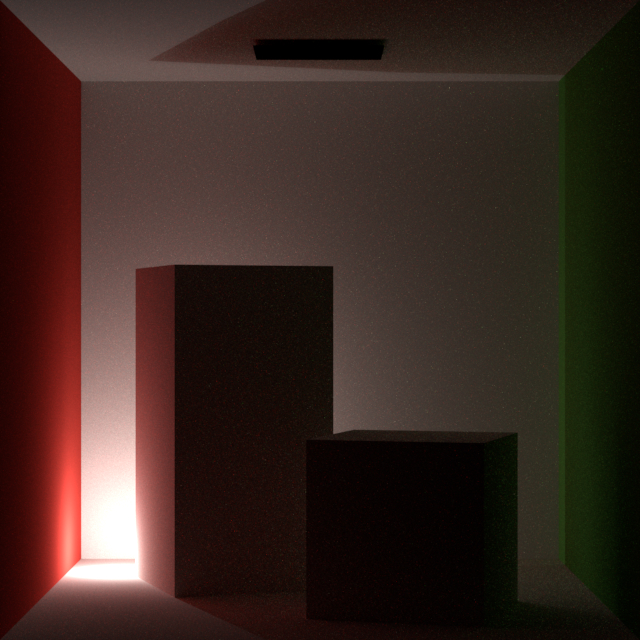
\includegraphics[width=\textwidth]{images/02-linear_lt_light02.jpg}
        \caption*{\(a = 0.0\), \(b = 1.0\)}
        %\label{}
    \end{subfigure}
    \hfill
    \begin{subfigure}[b]{0.24\textwidth}
        \centering
        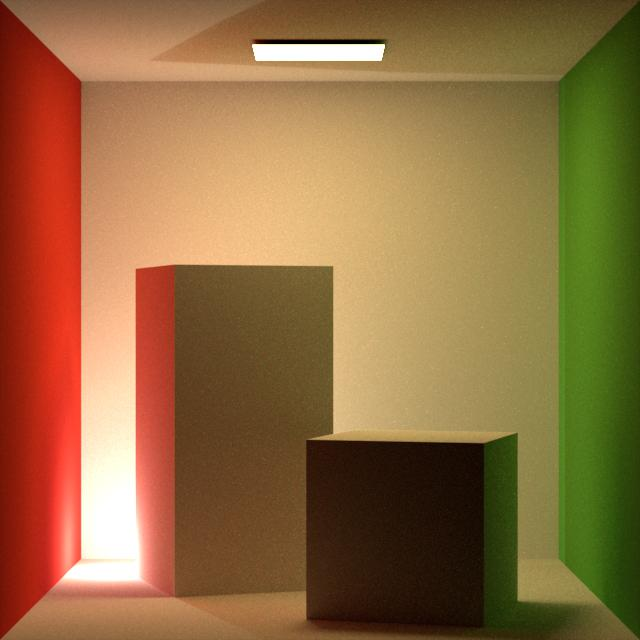
\includegraphics[width=\textwidth]{images/02-linear_lt_comb.jpg}
        \caption*{\(a = 1.0\), \(b = 1.0\)}
        %\label{}
    \end{subfigure}
    \hfill
    \begin{subfigure}[b]{0.24\textwidth}
        \centering
        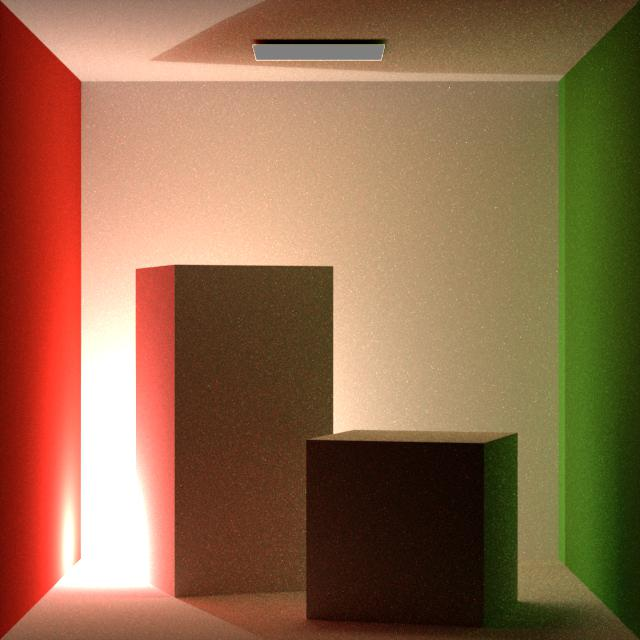
\includegraphics[width=\textwidth]{images/02-linear_lt_comb2.jpg}
        \caption*{\(a = 0.5\), \(b = 2.0\)}
        %\label{}
    \end{subfigure}
    \caption{Demonstration of the linearity of light transport. The scene displayed here has two light sources: on the ceiling and in the back corner. This means that its light transport can be captured using two basis images \(x_1\) and \(x_2\). Each of the above images was then created using a linear combination of the basis images: \(a \cdot x_1 + b \cdot x_2\)}
    \label{fig:background_linear_lt}
\end{figure}

As a consequence, radiance incoming onto a given camera sensor can be determined by the \textit{light transport (LT) matrix} \(A\):

\begin{equation}
    \label{eq:lt_matrix}
    A = \begin{bmatrix}
        c_{11} & c_{21} & c_{31} & \dots & c_{m1} \\
        c_{12} & c_{22} & c_{32} & \dots & c_{m2} \\
        c_{13} & c_{23} & c_{33} & \dots & c_{m3} \\
        \vdots & \vdots & \vdots & \ddots & \vdots \\
        c_{1n} & c_{2n} & c_{3n} & \dots & c_{mn}
    \end{bmatrix}
\end{equation}

where \(m\) is the number of light sources in a scene, \(n\) is the number of pixels in the camera sensor and \(c_{ij}\) is the value of the \(j\)-th pixel of an image that was rendered with only the \(i\)-th light source turned on. By taking a linear combination of the columns of the matrix it is then possible to obtain an image rendered by the corresponding combination of light sources.

In projection mapping, this matrix is usually extremely large because \(n\) corresponds to camera resolution and \(m\) corresponds to projector resolution. Also, in colorful images, each \(c_{ij}\) is a 3-dimensional vector. The two main challenges are therefore

\begin{itemize}
    \item Capturing the matrix
    \item Obtaining its inverse
\end{itemize}

In practice, it is impossible to capture the matrix by projecting a canonical basis because this would mean projecting with only a single pixel turned on and the signal-noise ratio of camera sensors is too high to capture such faint light. While it would be possible to project a different basis that is detectable by a camera, such a process would still be very time consuming. Methods for light transport capture usually rely on the fact that the LT matrix is often very sparse. In fact, the less inter-reflection there is in a scene, the sparser the matrix is. One example of a method that reconstructs the matrix using a limited number of samples is \citet{Peers2009}. Using that method it is possible to capture a matrix with \(m = 128^2\) using 991 measurements.

Inverting the matrix (or, more precisely, obtaining its pseudo-inverse because it is not generally square) is also practically impossible due to the size of the matrix. The solution is again to use the sparsity of the matrix to arrive at an estimate.

For example, \citet{Wetzstein2007} use the inverse light transport approach to implement a projection mapping method which works with arbitrary scenes and also compensates projector defocus which previously mentiones methods ignored. The drawbacks of this method are several hours long matrix acquisition process (during and after which the scene needs to stay static) and also the loss of some global illumination effects caused by estimates of both the LT matrix and its pseudo-inverse. Example results can be seen in fig. \ref{fig:background_wetzstein_result}.

\begin{figure}[ht]
    \centering
    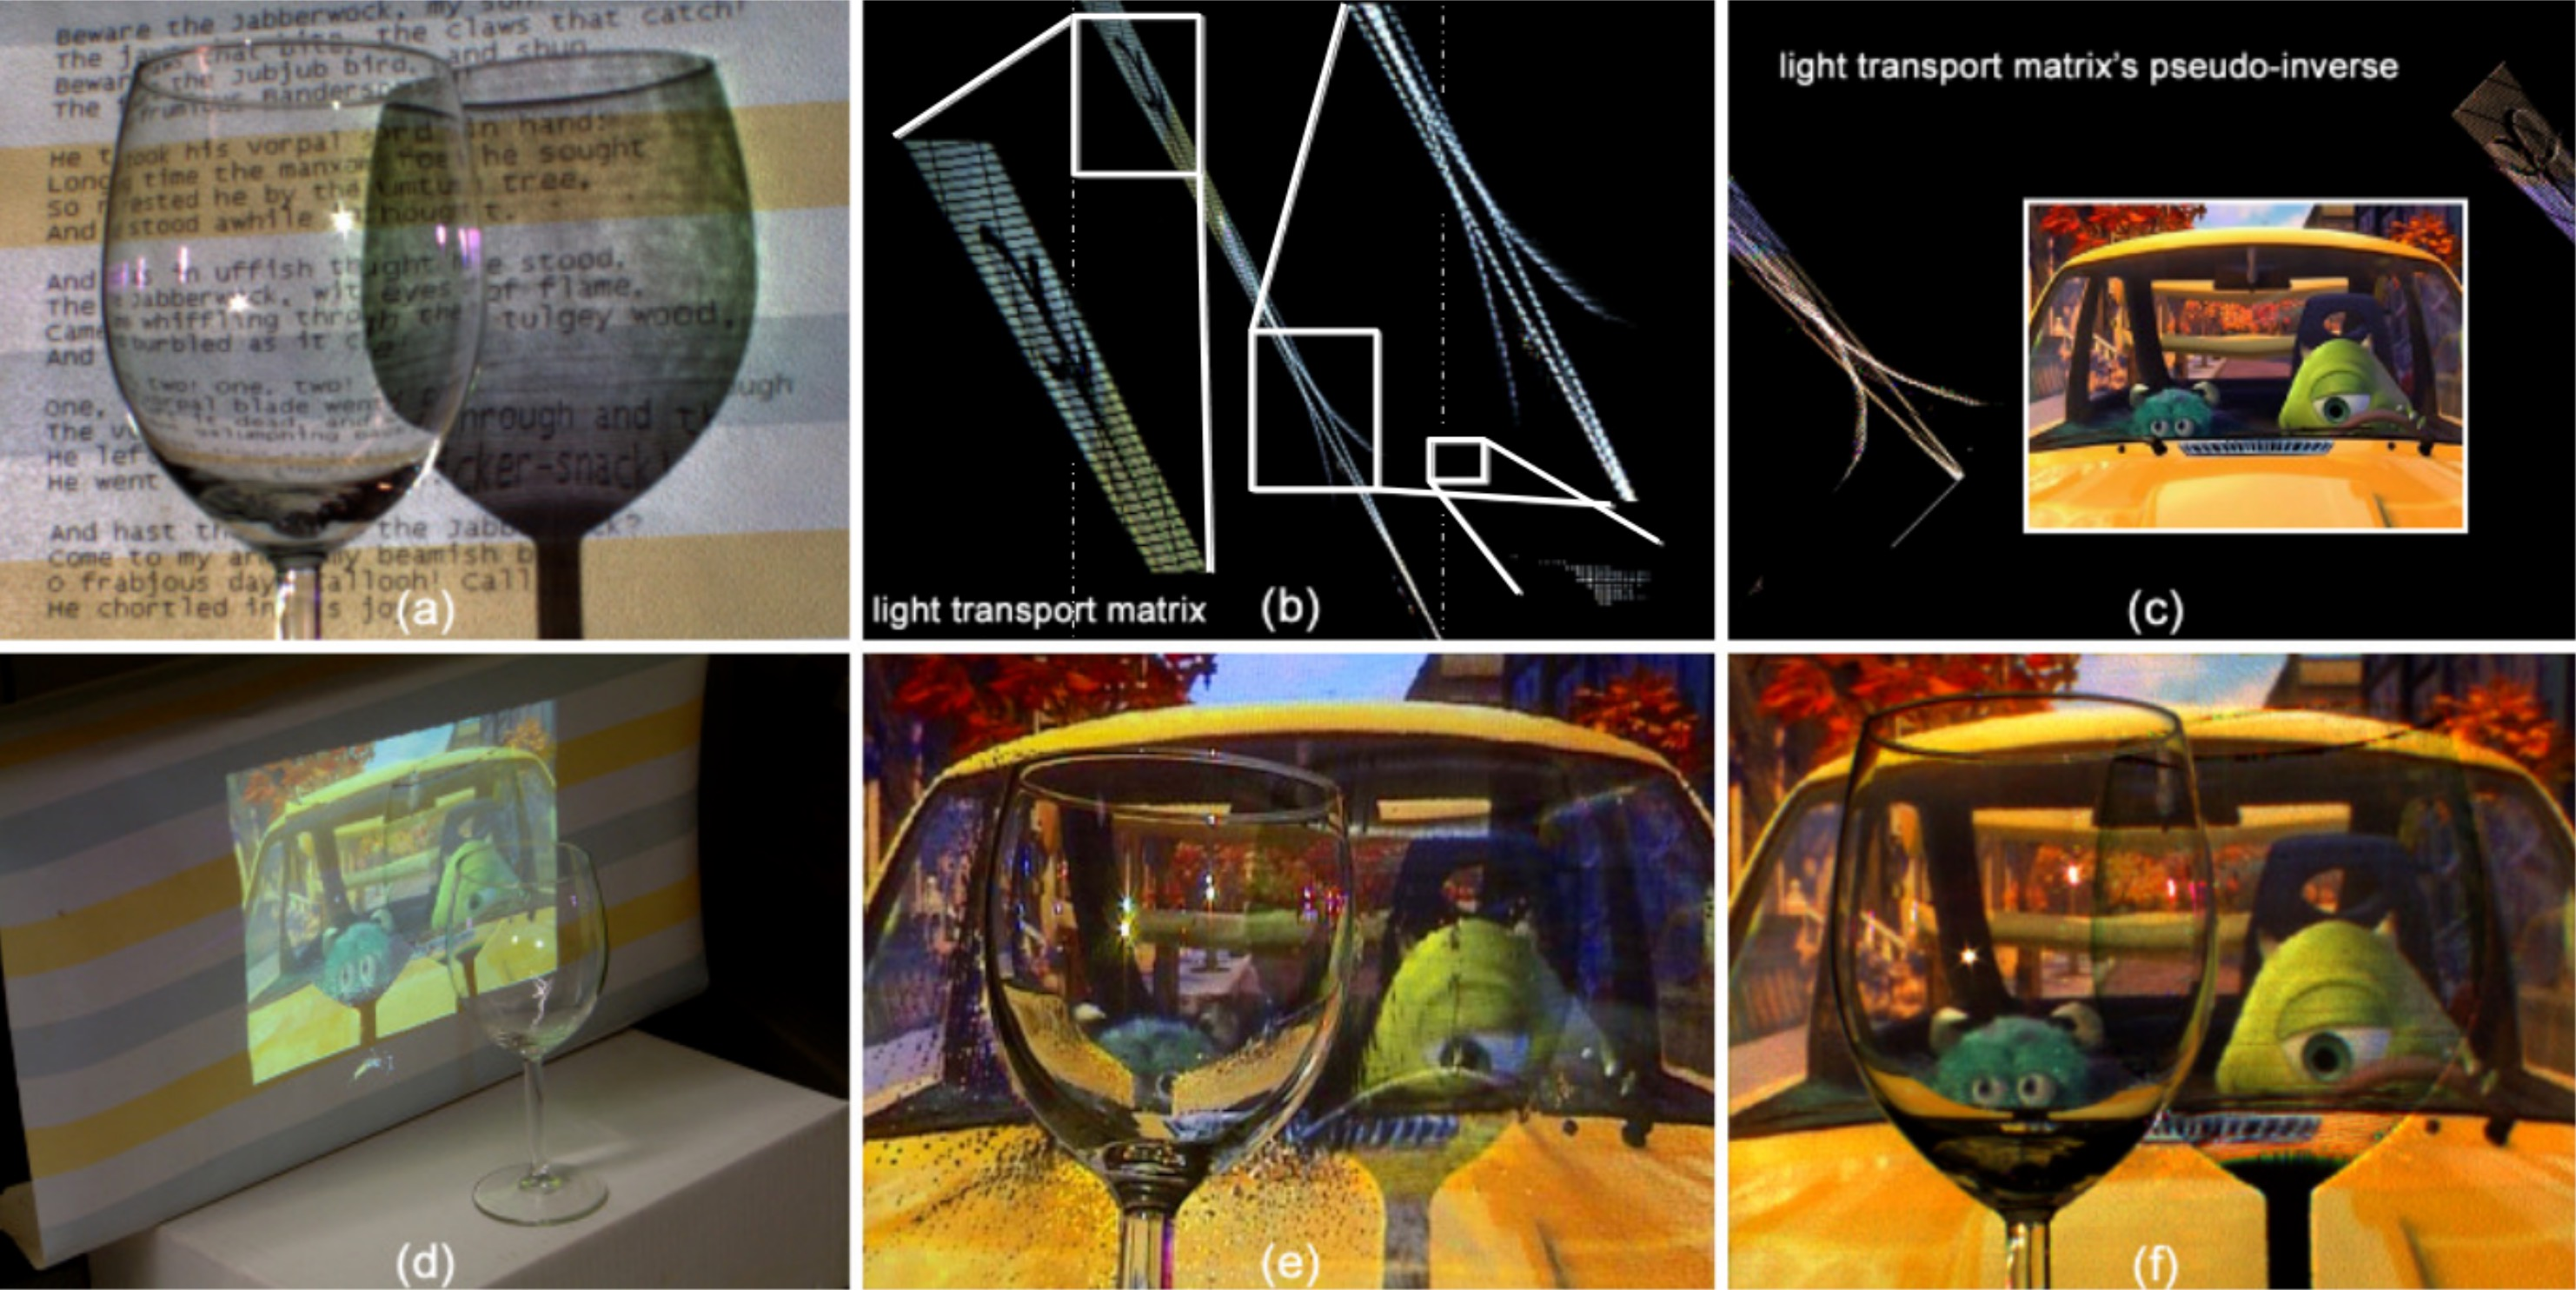
\includegraphics[width=0.8\textwidth]{images/02-wetzstein_result_compressed.jpg}
    \caption{Results of a projection mapping method by \citet{Wetzstein2007}. A wine glass in front of a colored wallpaper (a). The light transport matrix’s (b) pseudo-inverse (c, background) is approximated with a clustering scheme and allows a real-time compensation for displaying interactive content and movies (c) - from an angle (d), compensated with a conventional method (e) and with inverse light transport (f). Source: \citet{Wetzstein2007}}
    \label{fig:background_wetzstein_result}
\end{figure}

This concludes the section on projection mapping which was aiming to explain how to predict what an image will look like when projected onto a scene. We now move on to the second topic that our method builds on. This time we focus on what a texture is and how to generate new realizations of a given texture sample.

\section{Texture Synthesis}
\label{section:background-texture_synthesis}

As mentioned in section \ref{section:intro-key_idea}, the aim of this thesis is to advance the idea of content-based projection mapping of textures. As section \ref{section:background-projection_mapping} suggests, with current projector hardware it is not always possible to match the camera image with the desired appearance pixel by pixel while minimizing clipping errors. Hence in our method we loosen up the definition of image similarity. Textures are a great candidate to start with because two textures can have radically different pixel values in corresponding position but still look the same (see fig. \ref{fig:background_similar_textures} for an example).

\begin{figure}[ht]
    \centering
    \begin{subfigure}[b]{0.48\textwidth}
        \centering
        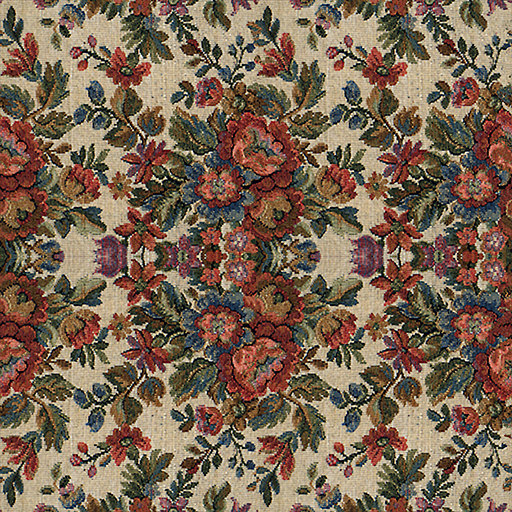
\includegraphics[width=\textwidth]{images/02-flowers1.png}
        \caption*{}
        %\label{}
    \end{subfigure}
    \hfill
    \begin{subfigure}[b]{0.48\textwidth}
        \centering
        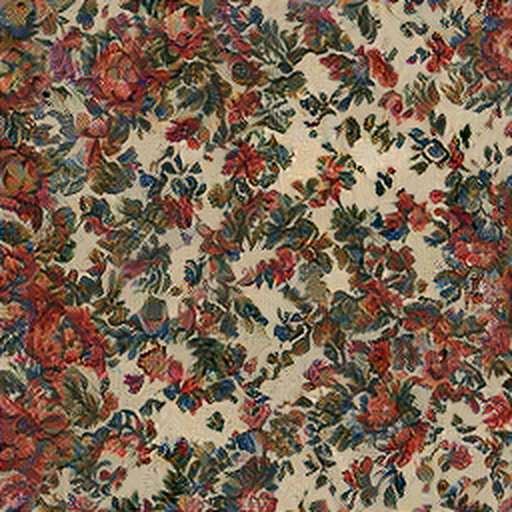
\includegraphics[width=\textwidth]{images/02-flowers2.png}
        \caption*{}
        %\label{}
    \end{subfigure}
    \caption{An example of two realizations of the same texture. The image on the right was created by a texture synthesis method of \citet{Gatys2015}. Texture source: \citet{Pixar128}, modified}
    \label{fig:background_similar_textures}
\end{figure}

But what exactly is a texture and what kind of image modifications can be done while preserving it? In this section, we provide an overview of texture synthesis research which is the second building block that our method relies on.

\subsection{Textures}
\label{section:background-texture_synthesis-textures}

Figures \ref{fig:intro_pixels_vs_stats} and \ref{fig:background_similar_textures} show examples of textures. Unfortunately, according to \citet{Raad2018} there is no universally accepted mathematical definition of what constitues a texture. Researchers who have attempted to characterize textures have usually defined them in terms of human vision. For example, \citet{Julesz1962}, one of the most prominent researchers in this field, has defined textures as classes of images that cannot be discriminated in preattantive (i.e. effortless or instantaneous) vision and then attempted to characterize them mathematically.

How should then one go about doing texture synthesis (i.e. generating new examples of a given texture class) when there is no formal definition of what a texture is? Existing methods can be divided into two categories based on how they approach this problem:

\begin{enumerate}
    \item Find a new candidate for texture definition which forms a texture model and then generate images according to that model. This category is also called \textit{parametric texture synthesis} or \textit{statistics-based texture synthesis} (because the models are usually statistical)
    \item Work without a model and instead define a procedure that turns a given texture example into a new one. This category is also called \textit{non-parametric texture synthesis} or \textit{patch-based texture synthesis} (because the procedure usually generates the texture image patch by patch)
\end{enumerate}

In the following sections we explain the theoretical background of both approaches to texture synthesis and describe the most important methods in each category. Specifically, we focus on strengths and weaknesses of each method and on how suitable it is for our purpose of projection mapping of textures as outlined in section \ref{section:intro-key_idea}. For a more in-depth review of the state of the art in texture synthesis, see \citet{Raad2018}.

\subsection{Patch-Based Texture Synthesis}
\label{section:background-texture_synthesis-patch_based}

We begin with patch-based texture synthesis because it is conceptually simpler and achieves very good results for particular kinds of textures. The basic idea was introduced by \citet{Efros1999} and was inspired by \citet{Shannon1948} and his use of a Markov chain to generate English text. Here is an example of Shannon's method (taken from \citet{Raad2018}):

\begin{itemize}
    \item in no ist lat whey cratict froure birs grocid pondenome of demonstures of the reptagin is regoactiona of cre
\end{itemize}

Analogously to two different texture realizations, this sentence is not English, but looks like it. It is generated letter by letter by sampling from a probability distribution of an English text sample conditioned on the previous \(n = 3\) letters.

In their texture synthesis method, \citet{Efros1999} generate an image pixel by pixel based on a probability distribution of the given texture sample. We will desribe how exactly this method works on an improved version of it, called \textit{image quilting}, which was introduced by \citet{Efros2001}.

\subsubsection{Image Quilting}
\label{section:background-texture_synthesis-patch_based-quilting}

\begin{figure}[ht]
    \centering
    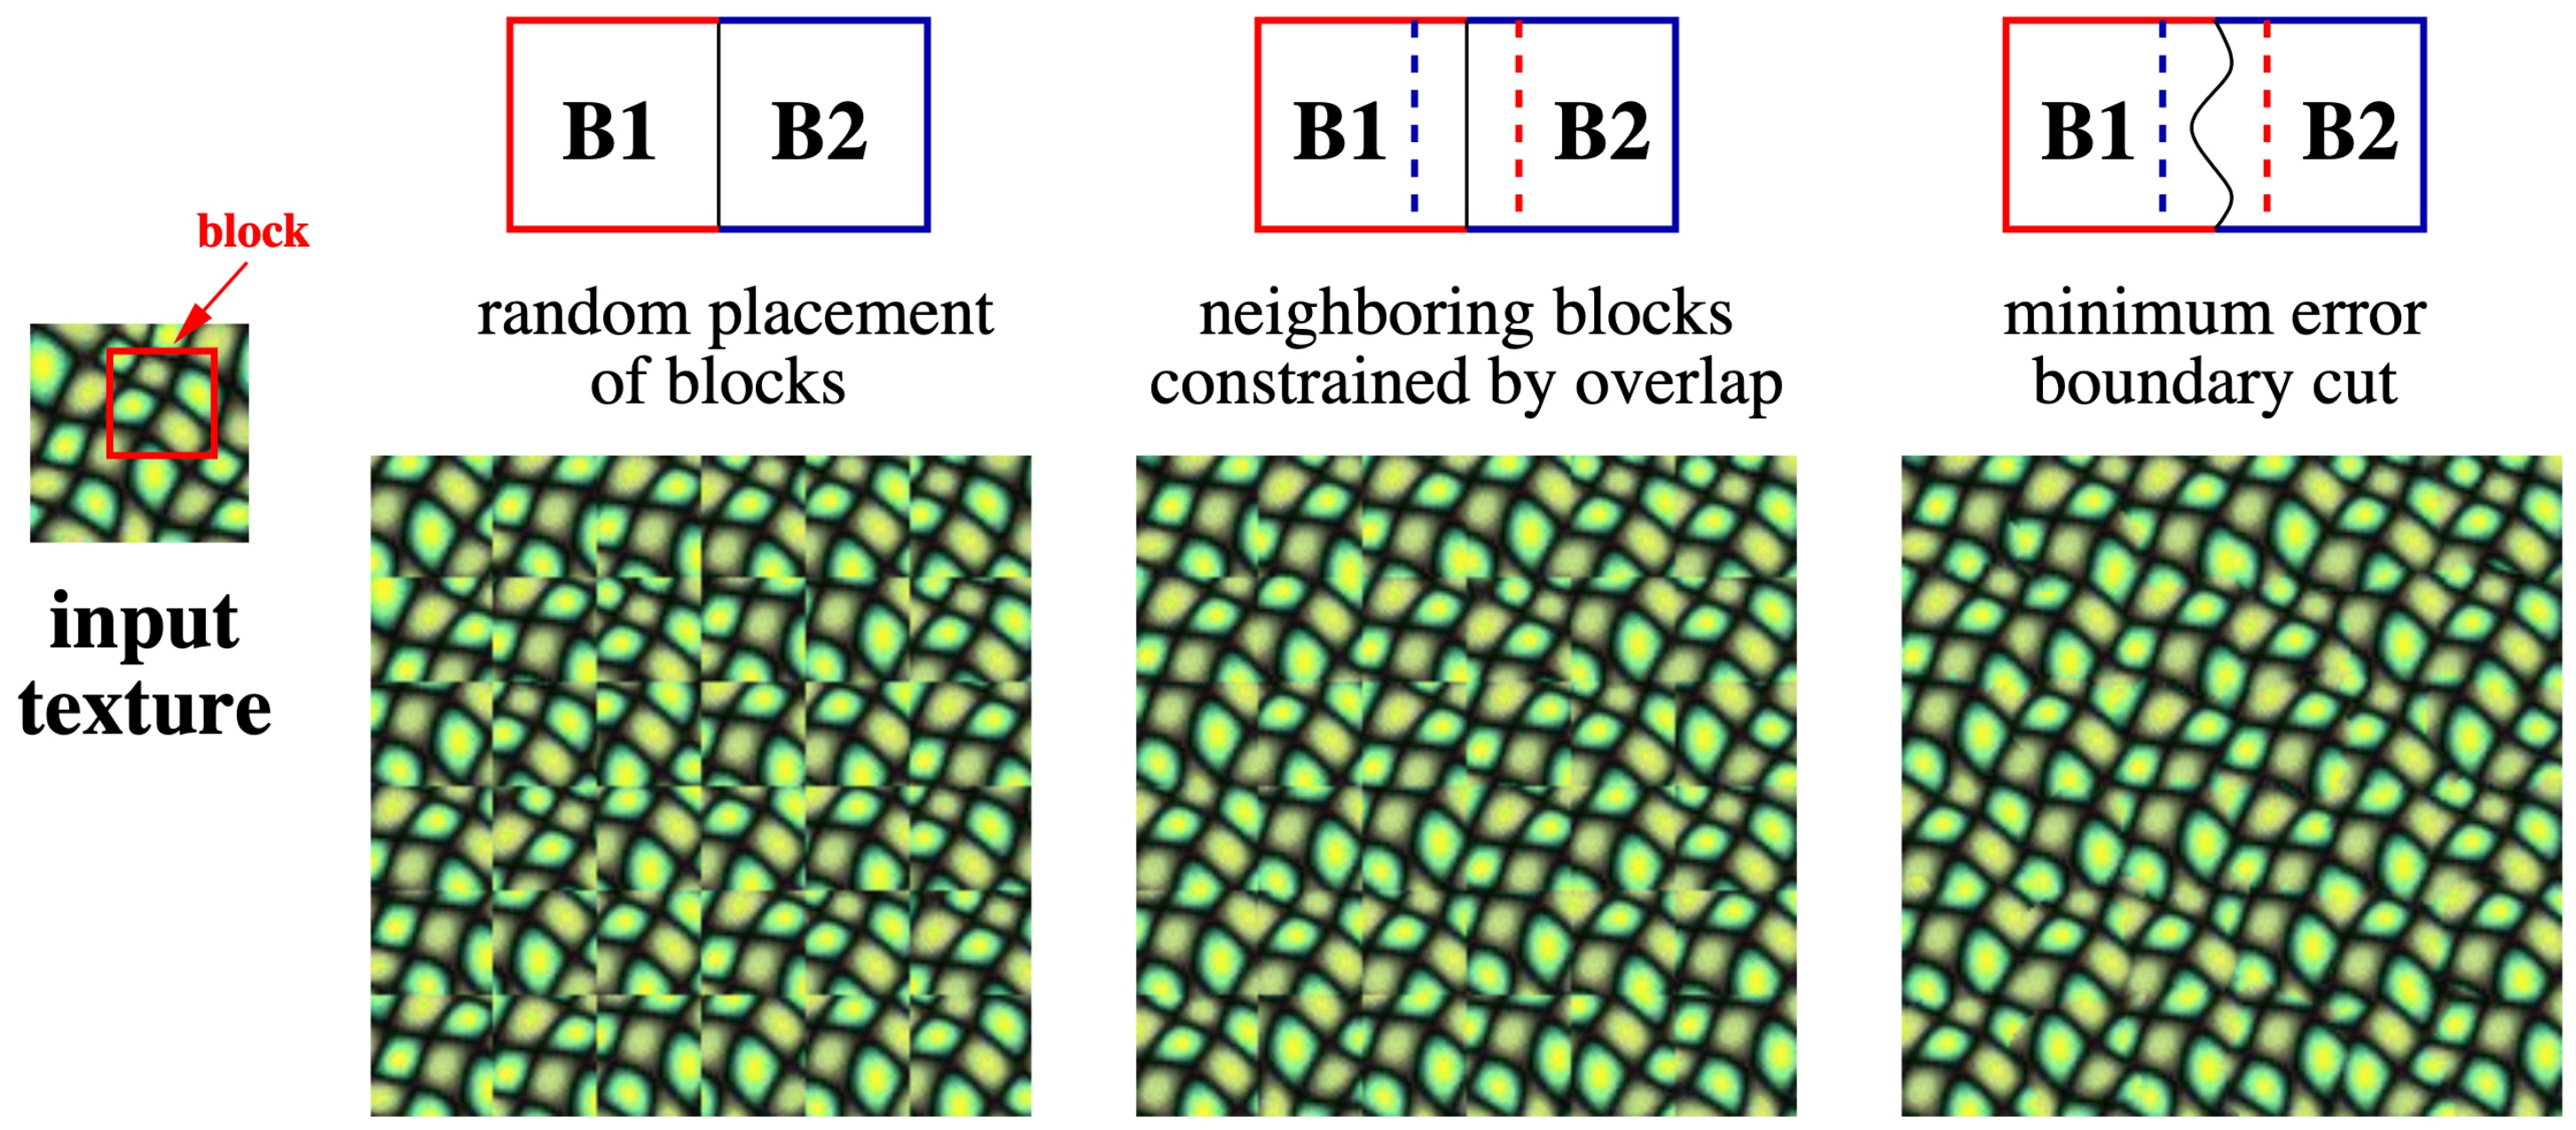
\includegraphics[width=\textwidth]{images/02-quilting_method_compressed.jpg}
    \caption{Illustration of image quilting. The leftmost image was generated by choosing block \(B_i\) at random. The middle image was generated by choosing a block with low pixel-wise error in an overlap with the previous block. The rightmost image was generated by choosing blocks as in the middle, only the new block is pasted along a minimum error path instead of a straight line.  Source: \citet{Efros2001}}
    \label{fig:background_quilting_method}
\end{figure}

Image quilting starts by splitting the input texture image into overlapping square blocks \(B_i\) of size \(k\) (a user-controlled parameter). Then it builds a new texture block by block in raster scan order (from the top left corner to the bottom right corner, row by row). A new block \(B^{\prime}\) is chosen at random from all \(B_i\) such that the pixel-wise error in overlapping areas (they use 1/6 of block area along the edge) with the block above \(B^{\prime}\) and to the left of \(B^{\prime}\) in below a certain threshold in the output image. Since many blocks usually satisfy this overlap constraint, one is picked at random. If \(B^{\prime}\) was pasted into the output image directly, the result would look blocky. Therefore \(B^{\prime}\) is pasted into the output image along a minimum error path inside the overlapping areas. This ensures that seams between block will be as subtle as possible. See fig. \ref{fig:background_quilting_method} for an illustration of the method.

\subsubsection{Pros and Cons}
\label{section:background-texture_synthesis-patch_based-pros_and_cons}

This method can achieve stunning visual results when the input texture is uniformly lit and contains large features, like pebbles or coffee beans. It is especially powerful when used on textures with regular structure, like a brick wall. See fig. \ref{fig:background_quilting_pros_cons} for an example.

However, it struggles with textures that have non-uniform illumination and that contain very small features, like sand or concrete. Failure cases usually manifest themselves by large areas that are directly copied from the input (so-called \textit{verbatim copying}) or areas that contain the same patch copied over and over (so-called \textit{garbage growing}). See fig. \ref{fig:background_quilting_pros_cons} for an example.

\begin{figure}[ht]
    \centering
    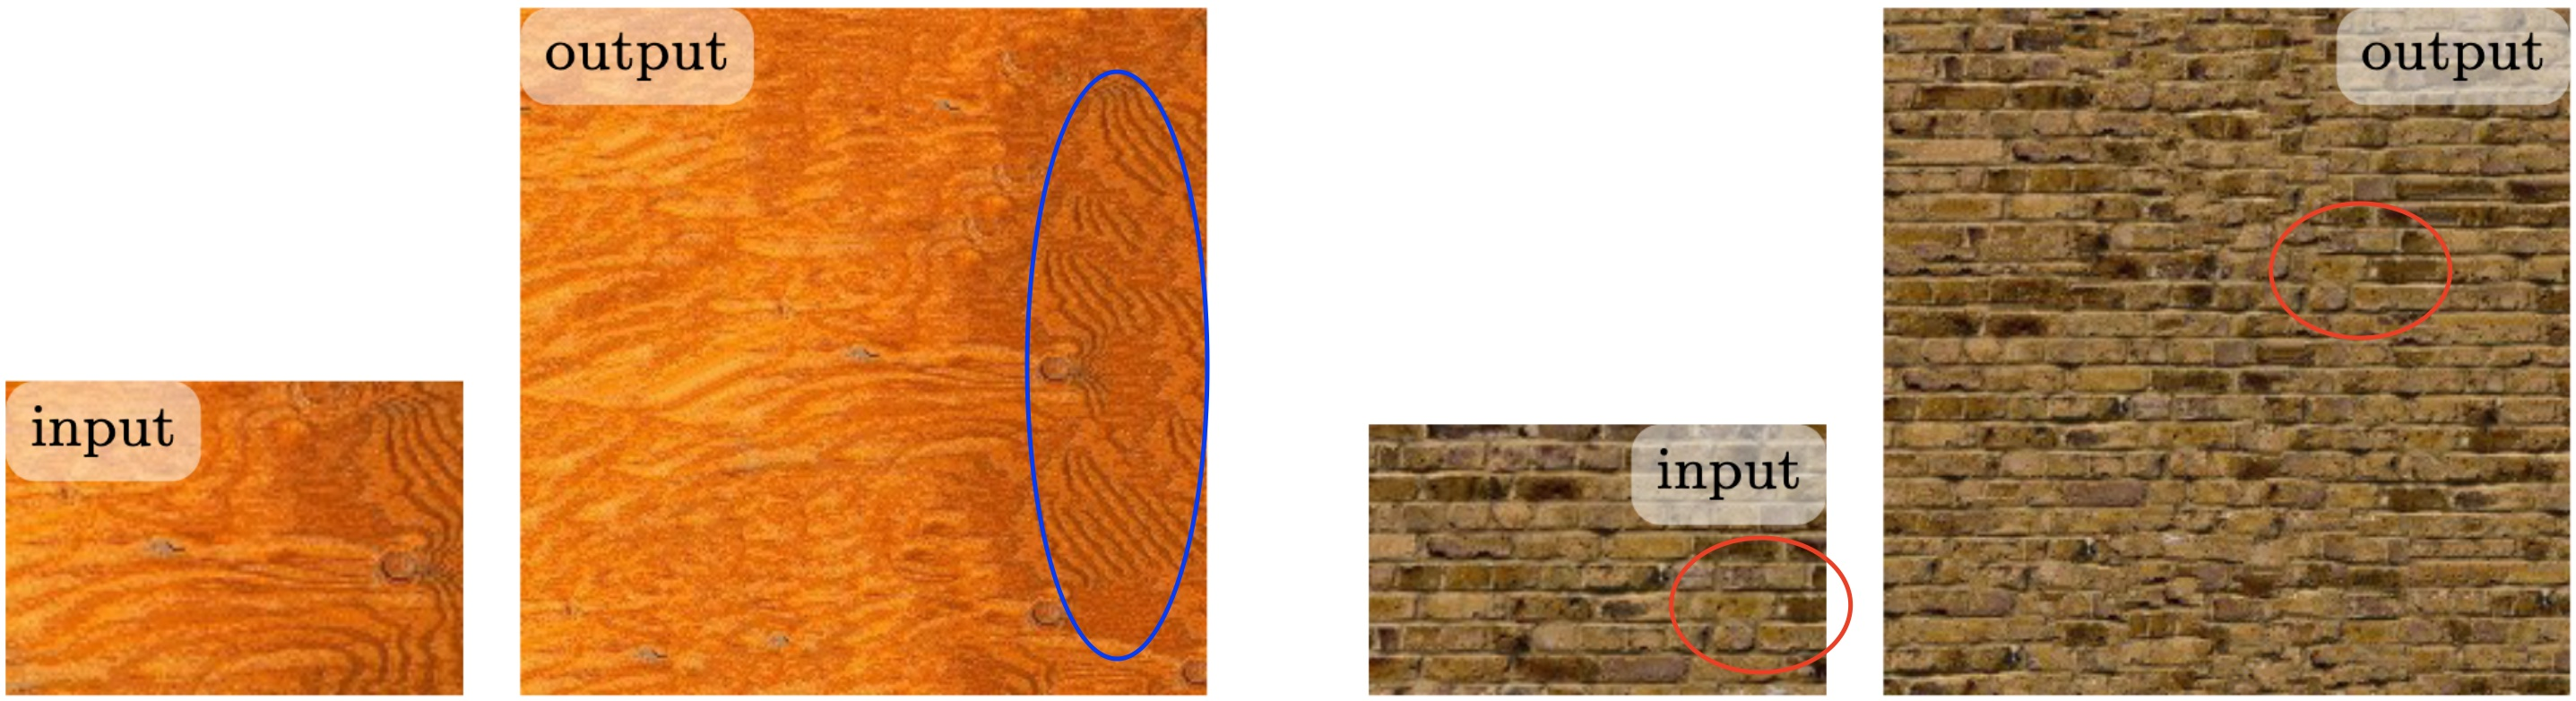
\includegraphics[width=\textwidth]{images/02-quilting_pros_cons_compressed.jpg}
    \caption{Examples of image quilting. On the left is a failure with the garbage growing effect highlighted in blue. On the right is a success. However, some verbatim copies (highlighted in red) are clearly visible in the rightmost image. Source: \citet{Raad2018}, highlighting own}
    \label{fig:background_quilting_pros_cons}
\end{figure}

Another drawback of this method is that its parameters need to be manually tuned based on the feature sizes and other properties of the input texture. There is also no underlying texture model that this method would work with which means that reasoning about it is somewhat less robust and limited to measuring heuristics such as the amount of verbatim copies and garbage in the output.

\subsubsection{Potential Usage in Projection Mapping}
\label{section:background-texture_synthesis-patch_based-projection_mapping}

Image quilting is surprisingly flexible to adapt for other uses than texture synthesis. The authors themselves showcase the possibility of using the method for style transfer. This is a problem that considers two input images and produces a third one which has the content of one image and style of the other. This can be achieved by adding a new term to the overlap error. In the case of style transfer, it takes the form of the difference in pixel intensities of the candidate patch and a corresponding patch of the target image. See fig. \ref{fig:background_quilting_transfer} for an example.

\begin{figure}[ht]
    \centering
    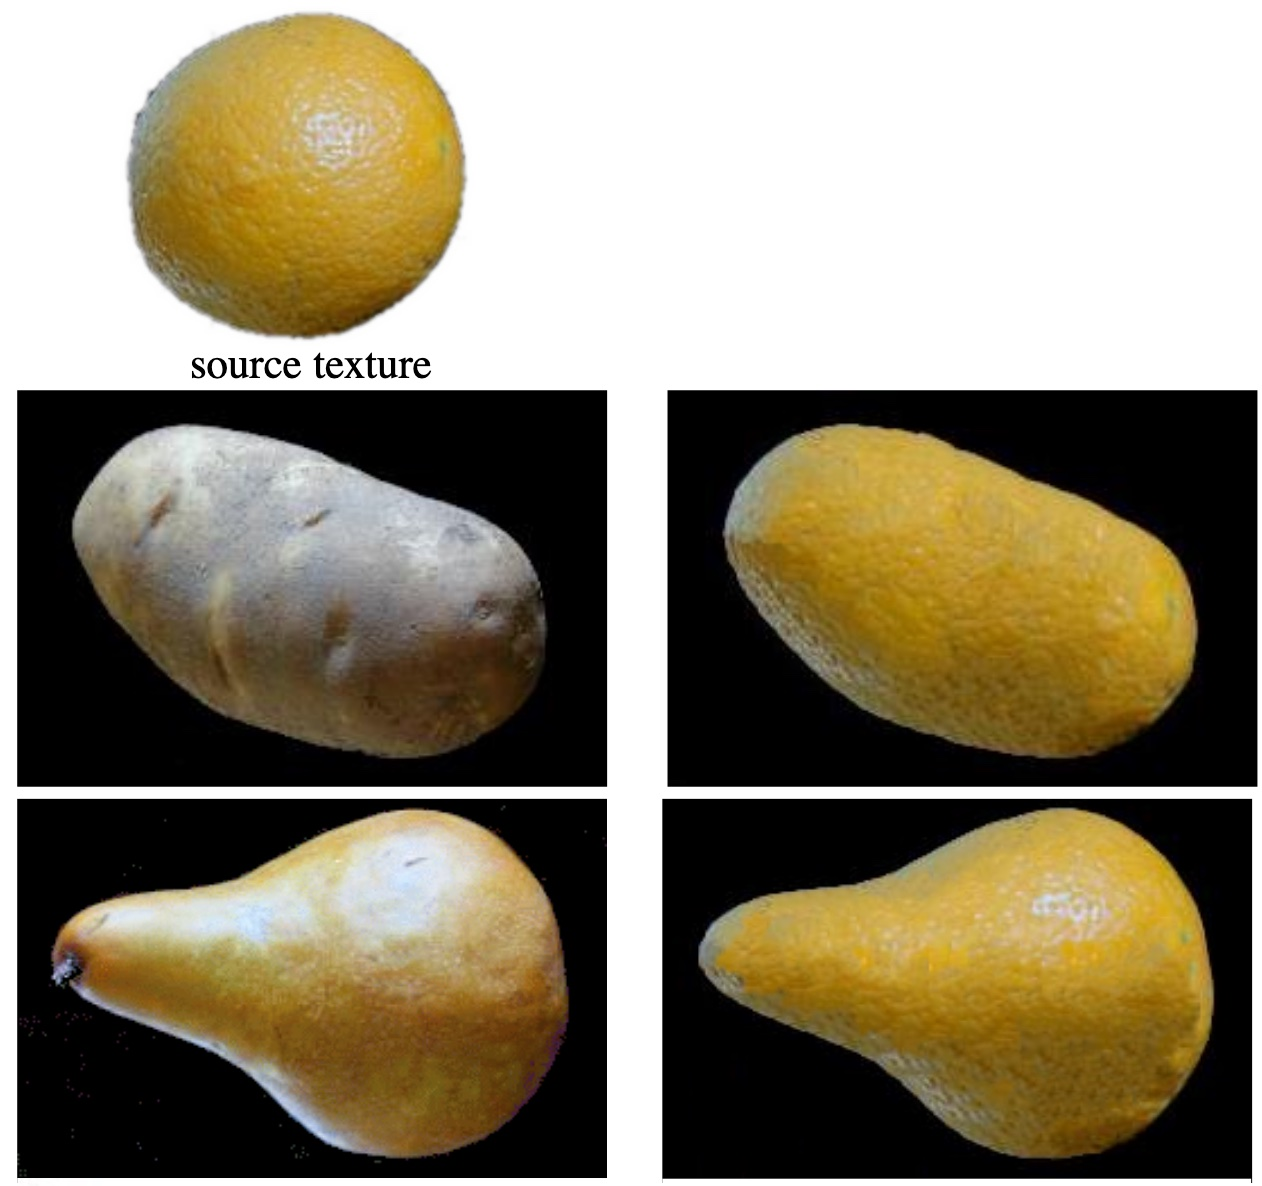
\includegraphics[width=0.6\textwidth]{images/02-quilting_transfer_compressed.jpg}
    \caption{Example of style transfer using image quilting. The output (right) is generated just like during texture synthesis except for two changes: 1) the output image size is chosen to be that of the target image (left) and 2) an extra term is added to the overlap error. This term represents the difference between the pixel intensities of the candidate patch and a corresponding patch of the target image. Source: \citet{Efros2001}}
    \label{fig:background_quilting_transfer}
\end{figure}

One could imagine using this method for projection mapping by modifying the overlap error term. Roughly speaking, the additional error term could be proportional to how difficult it would be to radiometrically compensate the candidate patch. More specifically, the candiate patch would first be radiometrically compensated and then the error would be set to the inverse distance of the compensation and the limit of the projector gamut. This could be built on top of methods such as \citet{Grundhofer2015} that assume 1:1 correspondence between projector image and camera image.

\subsection{Statistics-Based Texture Synthesis}
\label{section:background-texture_synthesis-statistics_based}

\begin{figure}[ht]
    \centering
    \begin{subfigure}[b]{0.3\textwidth}
        \centering
        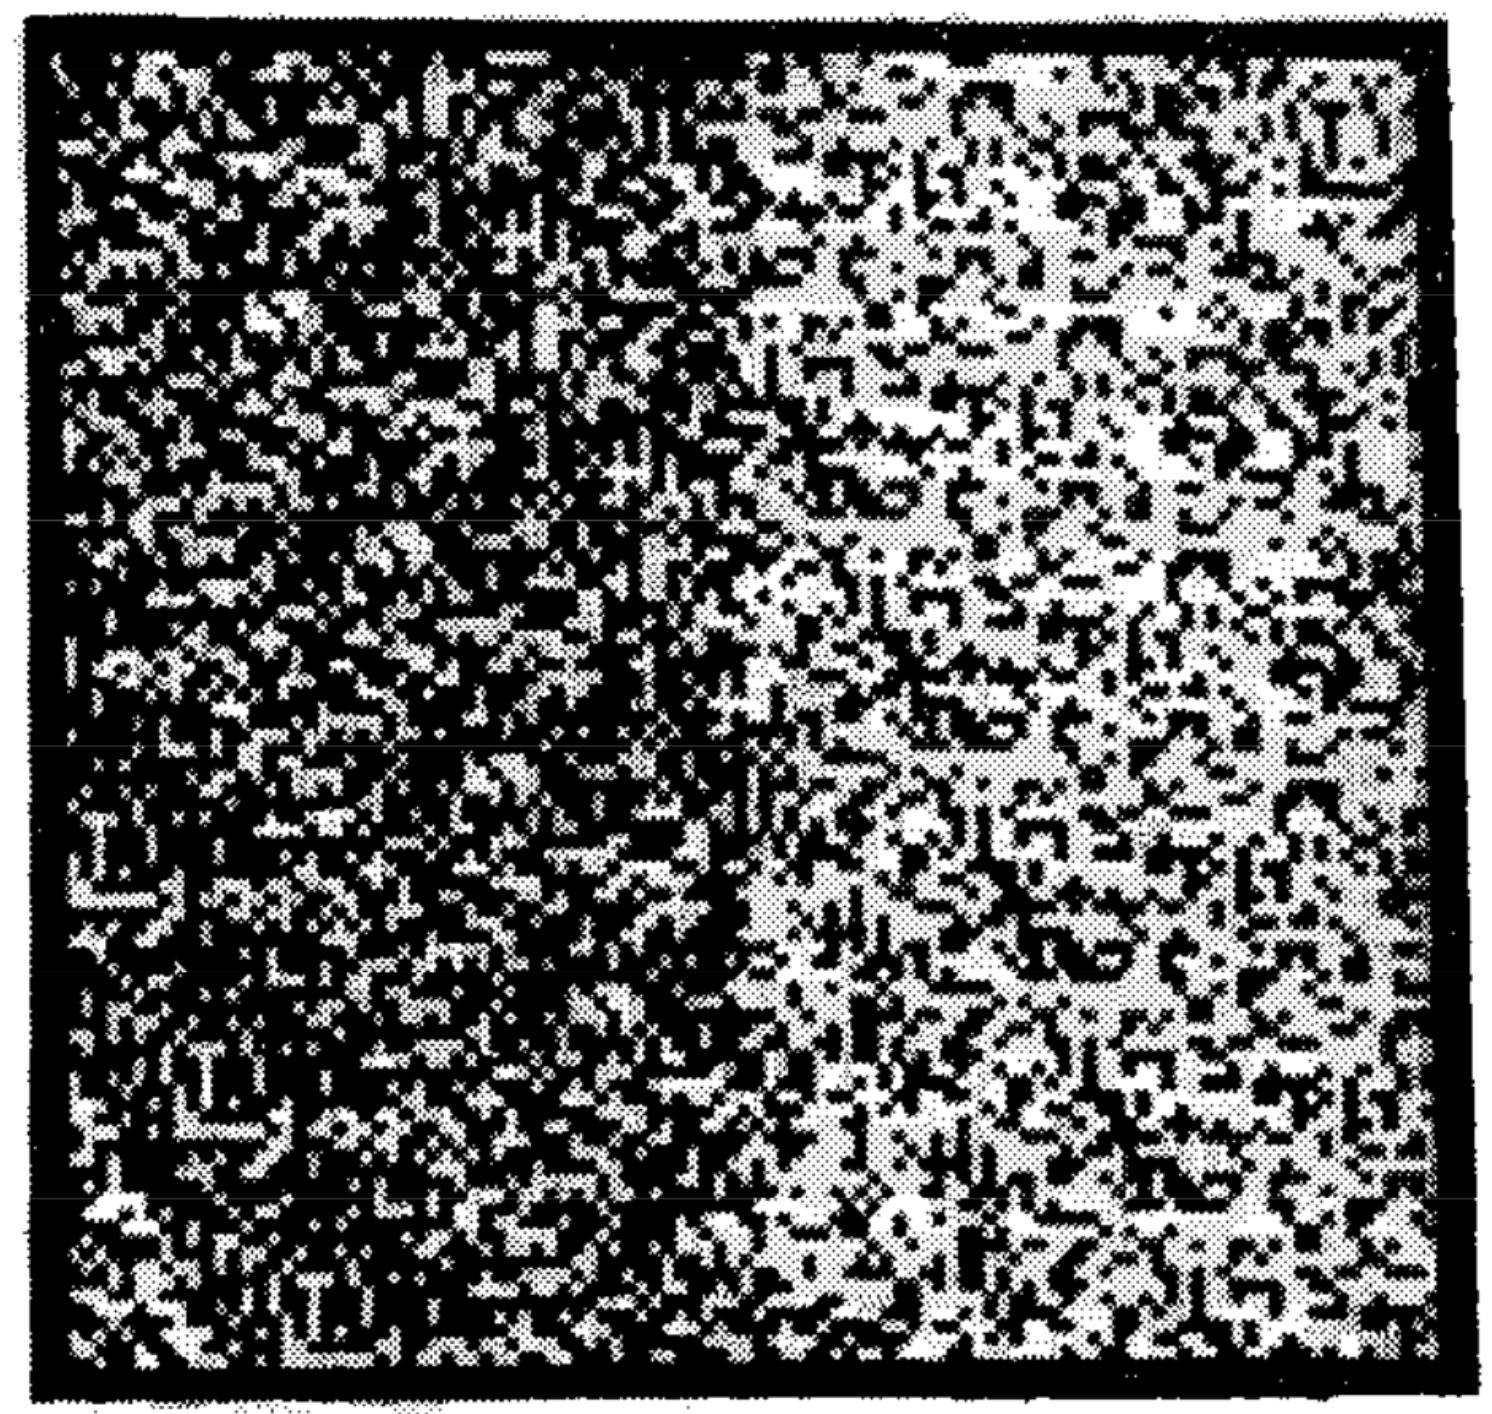
\includegraphics[width=\textwidth]{images/02-julesz-1st_order_compressed.jpg}
        \caption{}
        %\label{}
    \end{subfigure}
    \hfill
    \begin{subfigure}[b]{0.29\textwidth}
        \centering
        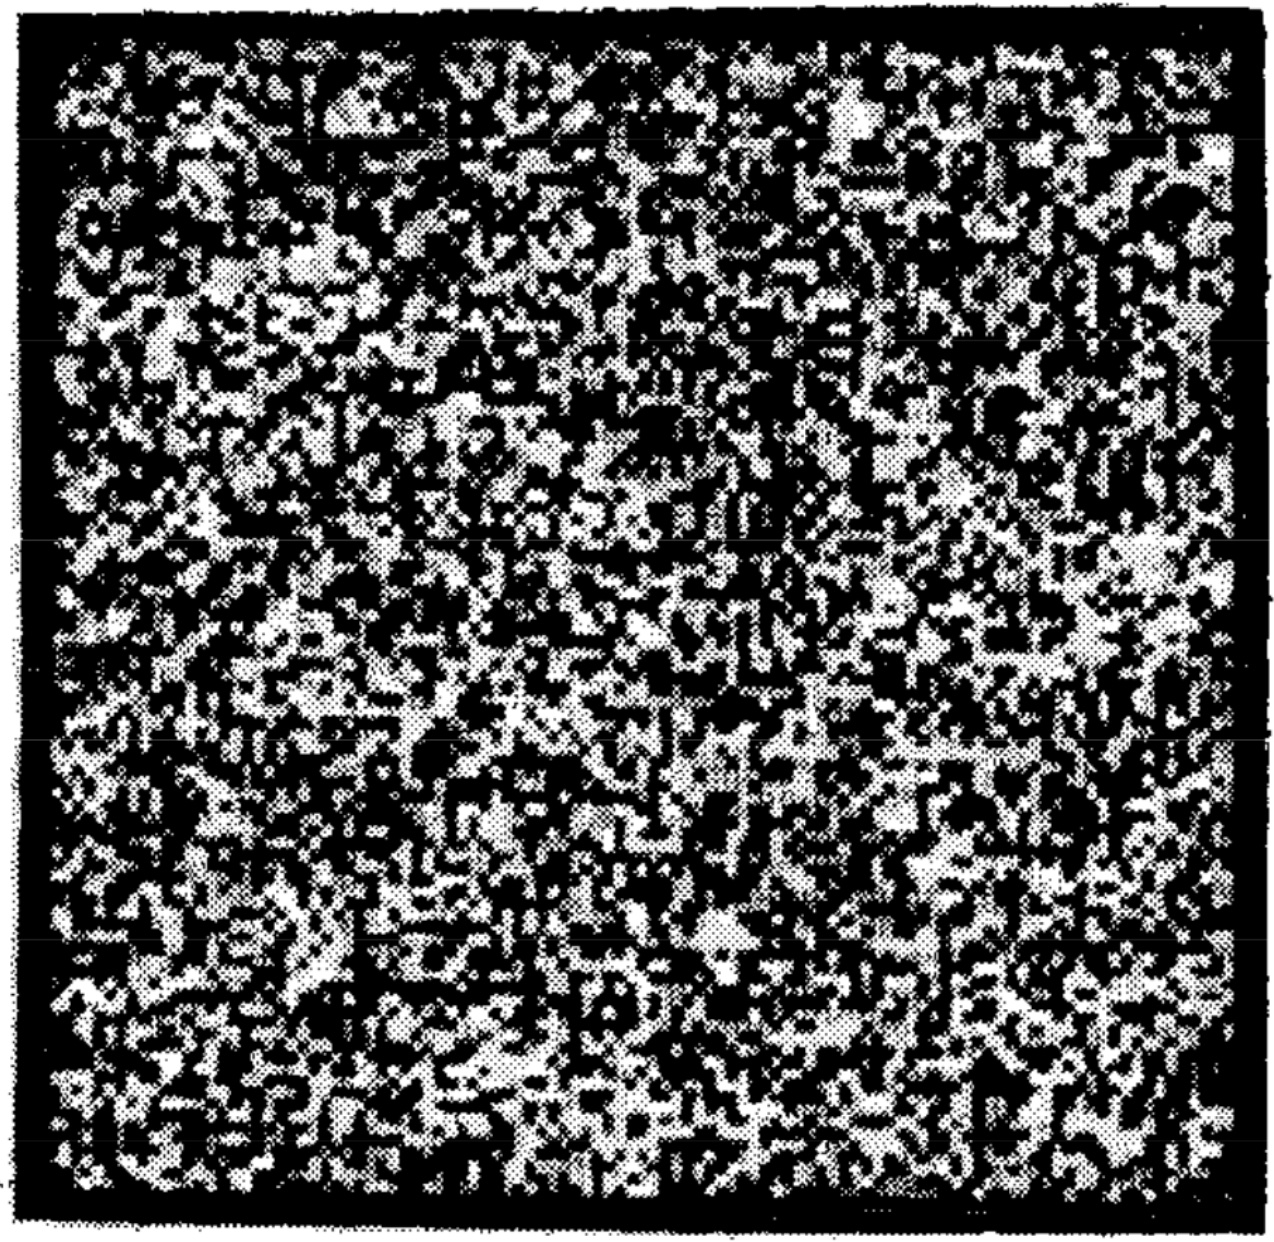
\includegraphics[width=\textwidth]{images/02-julesz-2nd_order_compressed.jpg}
        \caption{}
        %\label{}
    \end{subfigure}
    \hfill
    \begin{subfigure}[b]{0.39\textwidth}
        \centering
        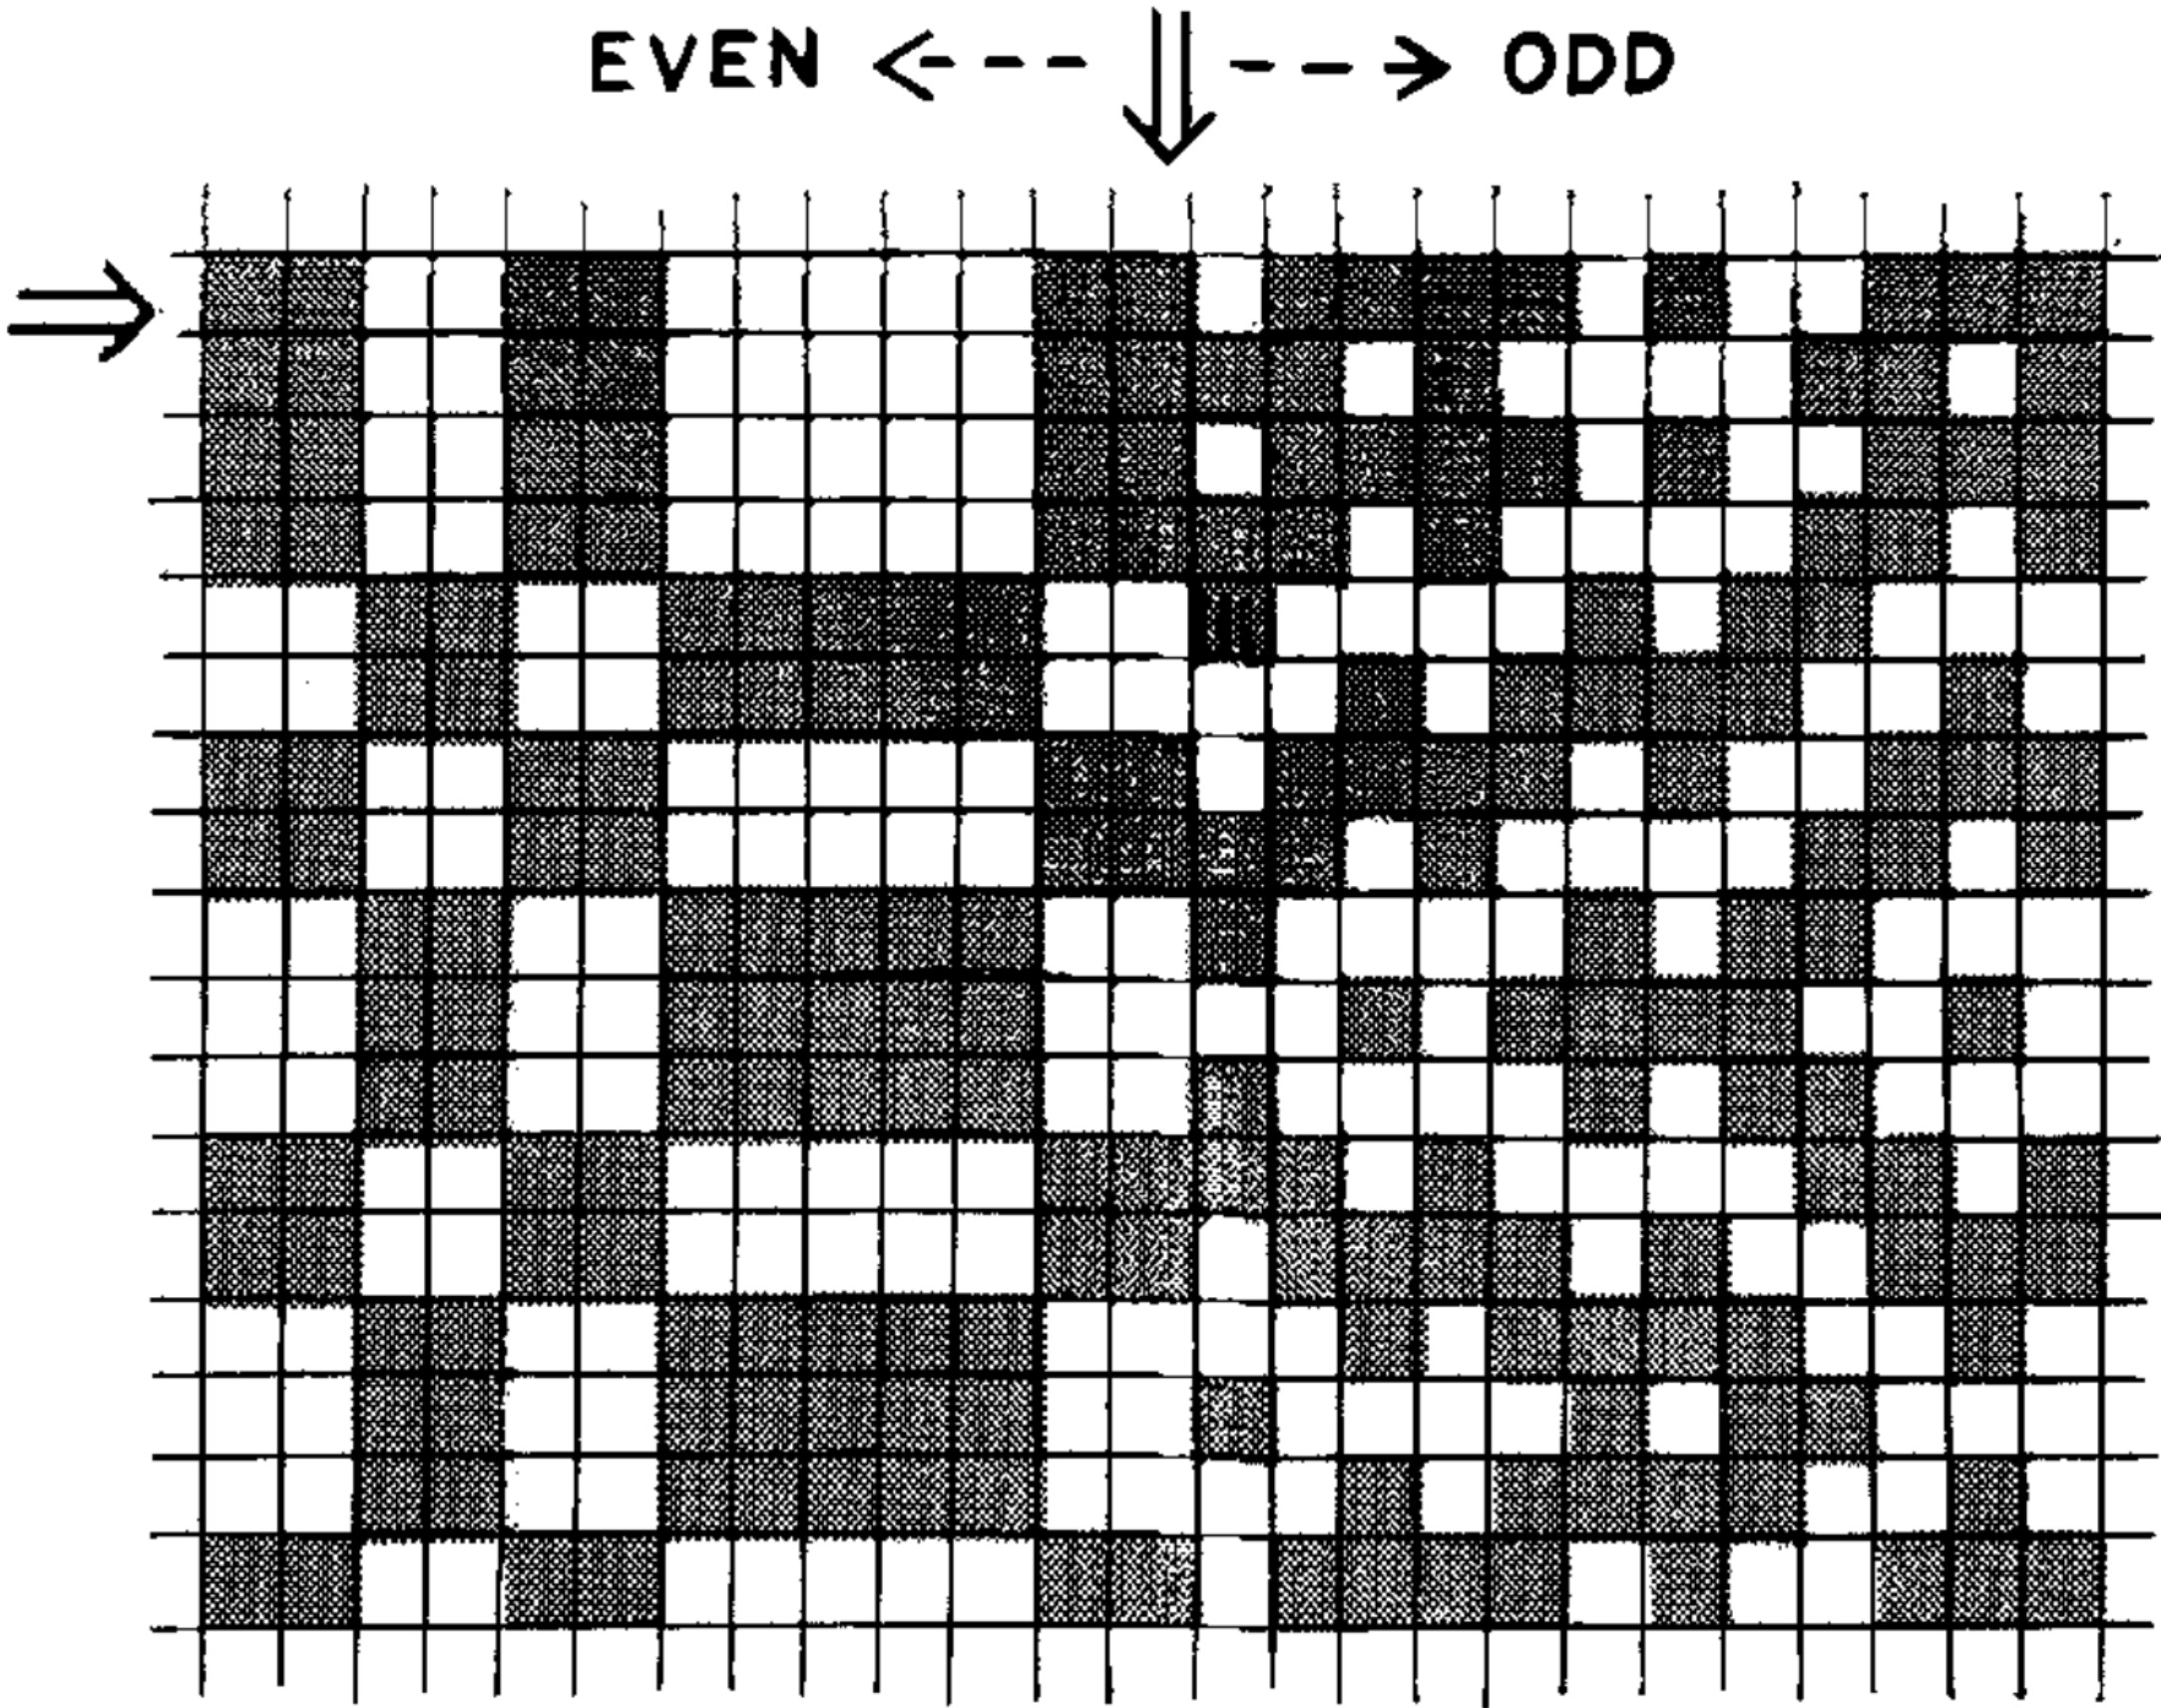
\includegraphics[width=\textwidth]{images/02-julesz-3rd_order_compressed.jpg}
        \caption{}
        %\label{}
    \end{subfigure}
    \caption{Image a) shows two textures with different first-order statistics. The left half contains black pixels with probabilty \(5/8\) and white pixels with probability \(3/8\) while the right half has the inverse distribution. Image b) shows two textures with identical second-order statistics. Specifically, there are four brightness levels in the image each with equal probability (first-order). Moreover, any two pixels are chosen independently (second-order). However, the probability \(P(k | i,j)\) of a pixel conditioned on two other pixels differs between the left and right half which makes third-order statistics different. Image c) shows two textures with identical third-order statistics, meaning that any three squares are chosen independently. However, the left half has \(2 \times 2\) patches with even number of black squares while the left half has an odd number of black squares per patch. This makes the textures easily distinguishable. Texture sources: \citet{Julesz1962} (a, b) and \citet{Julesz1973} (c)}
    \label{fig:background_julesz_textures}
\end{figure}

Statistics-based texture synthesis is an older and more established approach to generating new realizations of textures because it combines two goals:

\begin{itemize}
    \item Finding a mathematical characterization of textures
    \item Synthesizing new texture examples based on that characterization
\end{itemize}

As mentioned in section \ref{section:background-texture_synthesis}, a formal texture model should be compatible with the notion that textures are classes of images that are indistinguishable in preattentive vision. A famous attempt at such a model was introduced by \citet{Julesz1962} who formulated a hypothesis that two textures with identical second-order statistics are preattentively indistinguishable from each other (see fig. \ref{fig:background_julesz_textures} for an example). This hypothesis was later disproved in \citet{Julesz1973} by counter-examples of distinguishable textures with identical third-order statistics (also fig. \ref{fig:background_julesz_textures}). However, the distinguishing features in those counter-examples are local. A modified Julesz hypothesis says that "the pre-attentive textural system cannot globally compute third- or higher-order statistics" (\citet{Julesz1981}) and the idea that global statistics characterize textures well is still prevalent today. See fig. \ref{fig:background_statistics_example} for an illustration of how global statistics can be used for texture synthesis.

\begin{figure}[ht]
    \centering
    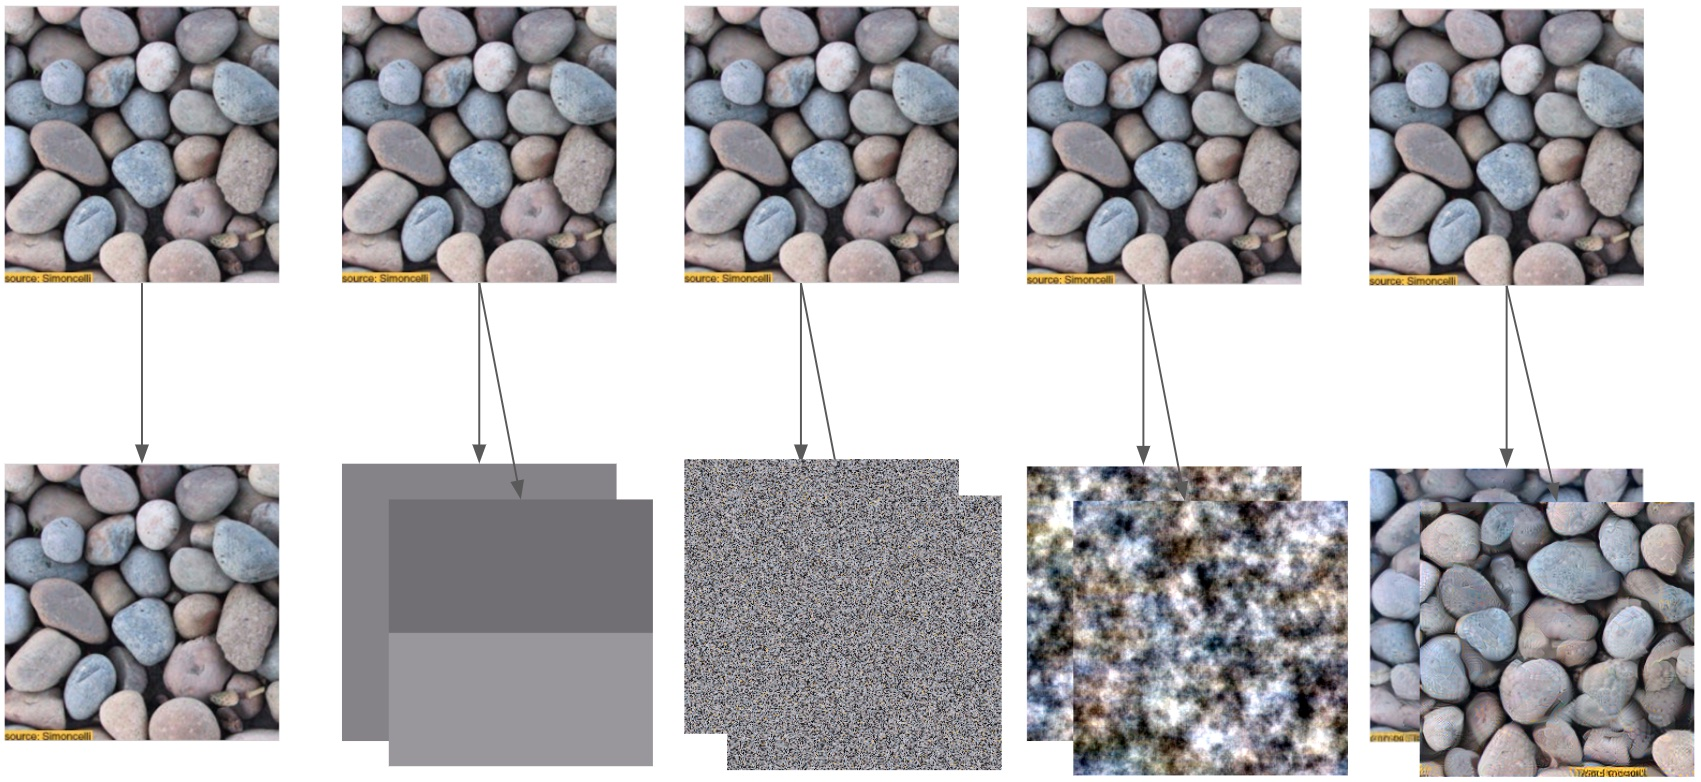
\includegraphics[width=\textwidth]{images/02-statistics_example_compressed.jpg}
    \caption{Illustration of texture synthesis via global image statistics. The leftmost image shows an example generated by keeping every pixel identical. The middle-left image shows an example that uses identical average color as a descriptive statistic. The middle image uses first-ordr statistics by simply shuffling the pixels of the input. The middle-right image uses a method by \citet{Galerne2011} which keeps Fourier modulus identical while randomizing the phase. The rightmost image shows a recent method by \citet{Gatys2015} that uses the Gram matrices of CNN activations as a descriptive statistic. Texture source: \citet{Gatys2015}}
    \label{fig:background_statistics_example}
\end{figure}

In line with the modified Julesz hypothesis, we can see from the examples above that while some synthesis methods are good at creating textures with distinct local features but struggle with more homogeneous texture (e.g. \citet{Efros2001} in fig. \ref{fig:background_quilting_pros_cons}), others are the opposite (e.g. \citet{Galerne2011} and its failure on a macro-texture in fig. \ref{fig:background_statistics_example}). In literature, texture with distinct local features are called \textit{macro-texture} and more homogeneous textures are called \textit{micro-texture}. For a long time there was no method that could reliably generate both types of texture. However, a recent statistics-based method by \citet{Gatys2015} achieves very good results on both micro-textures and macro-textures and we will now provide its overview and explain how it could be used in projection mapping.

\subsubsection{Texture Synthesis Using Convolutional Neural Networks}
\label{section:background-texture_synthesis-statistics_based-synthesis_using_cnns}

\citet{Gatys2015} have introduced a method for texture synthesis that defines a set of statistics that can be computed from an image and then generates new examples of a given texture by imposing those statistics on white noise images. This happens in an optimization loop that minimizes a loss function which represents the difference between the statistics of the generated image and the input texture (see fig. \ref{fig:background_gatys_method} for an illustration).

\begin{figure}[ht]
    \centering
    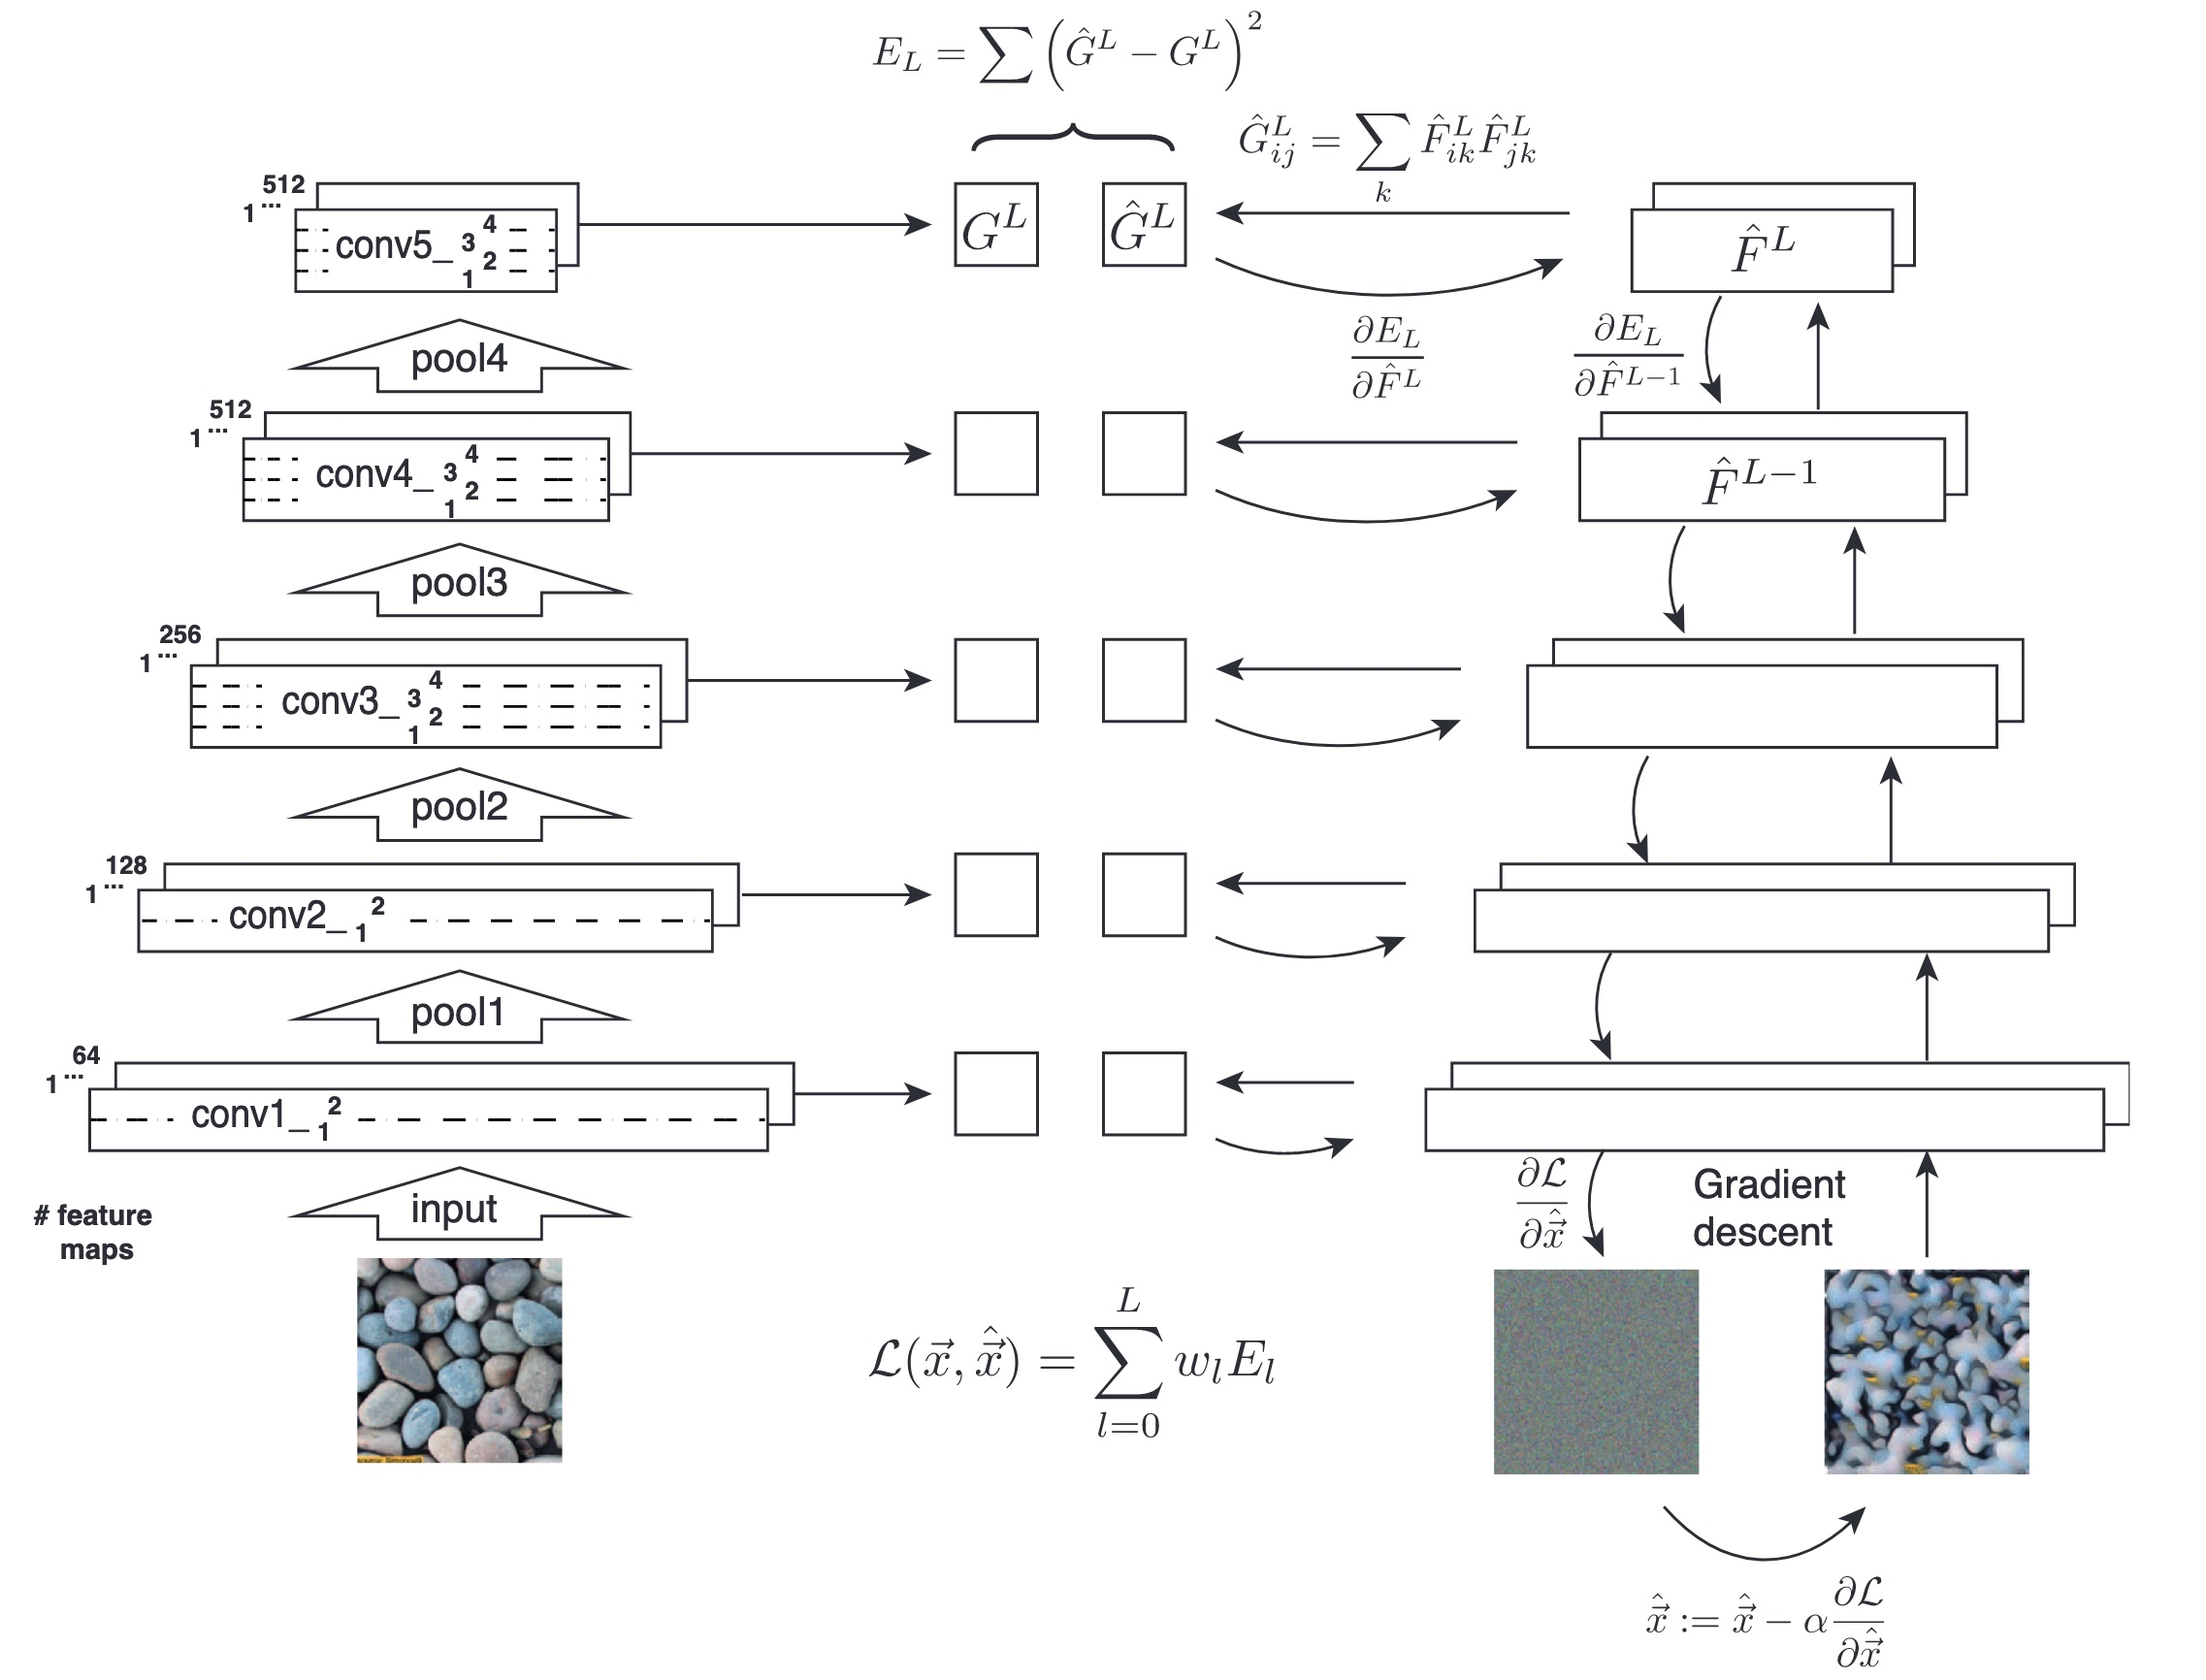
\includegraphics[width=\textwidth]{images/02-gatys_method_compressed.jpg}
    \caption{Illustration of CNN-based texture synthesis by \citet{Gatys2015}. At the bottom we can see the input texture, the initial white noise image and the progressively refined image. The diagram above represents the computation of the CNN activations and their Gram matrices \(G\). The loss \(\mathcal{L}\) that drives the optimization via gradient descent is defined as a weighted sum of the differences between Gram matrices of individual CNN layers. Source \citet{Gatys2015}}
    \label{fig:background_gatys_method}
\end{figure}

The set of statistics is computed using a \textit{convolutional neural network} (abbreviated as CNN and covered in more detail in appendix \ref{chapter:appendix-cnns}) which is trained on an image classification task. It is determined by the activations after each pooling layer of the VGG-19 CNN by \citet{Simonyan2014}. These activations, however, contain spatial information of where each feature is located in the texture. This is not desirable because textures are stationary (i.e. their features can be shuffled around without making them a different texture). In order to remove this spatial information, activations are correlated with each other within each layer, forming a so-called \textit{Gram matrix}. Gram matrices of VGG-19 activations therefore constitute a set of statistics completely describing a texture.

To synthesize a new example of a given texture, gradient-based loss optimization is used. The loss is defined as a weighted mean square error between the statistics the input texture and the image being optimized. The L-BFGS optimizer is used to drive the optimization process. See fig. \ref{fig:background_gatys_method} for an illustration of how this method works.

\subsubsection{Pros and Cons}
\label{section:background-texture_synthesis-statistics_based-pros_and_cons}

\begin{figure}[ht]
    \centering
    \begin{subfigure}[b]{0.8\textwidth}
        \centering
        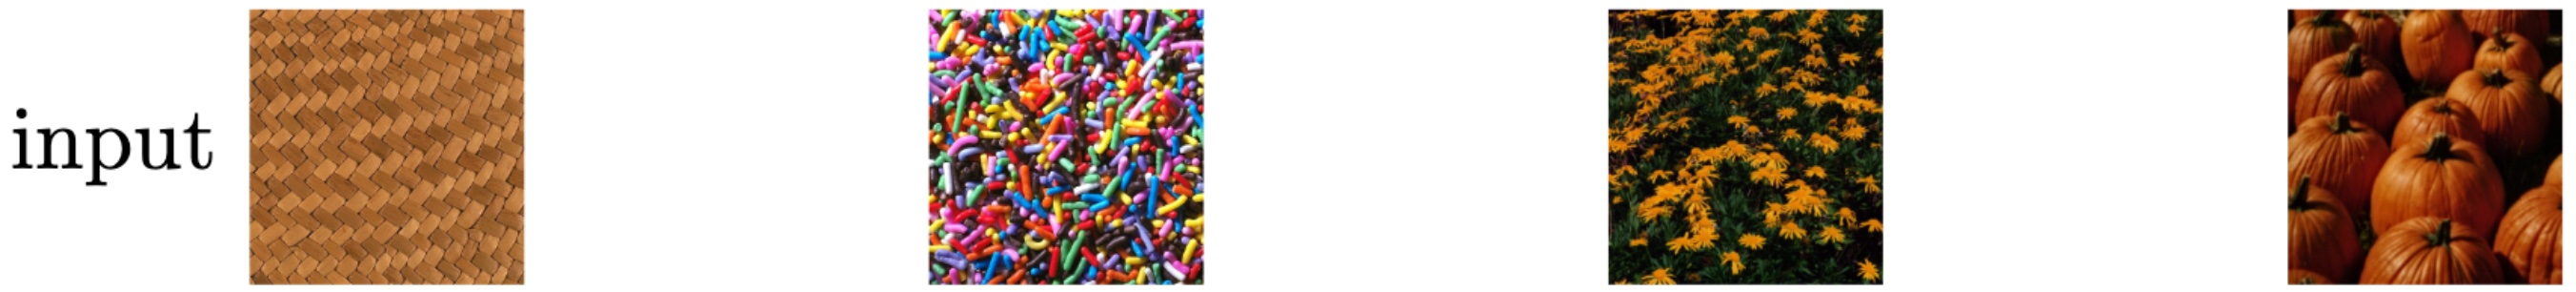
\includegraphics[width=\textwidth]{images/02-big_comparison_input_compressed.jpg}
        \caption*{}
        %\label{}
    \end{subfigure}
    
    \begin{subfigure}[b]{\textwidth}
        \centering
        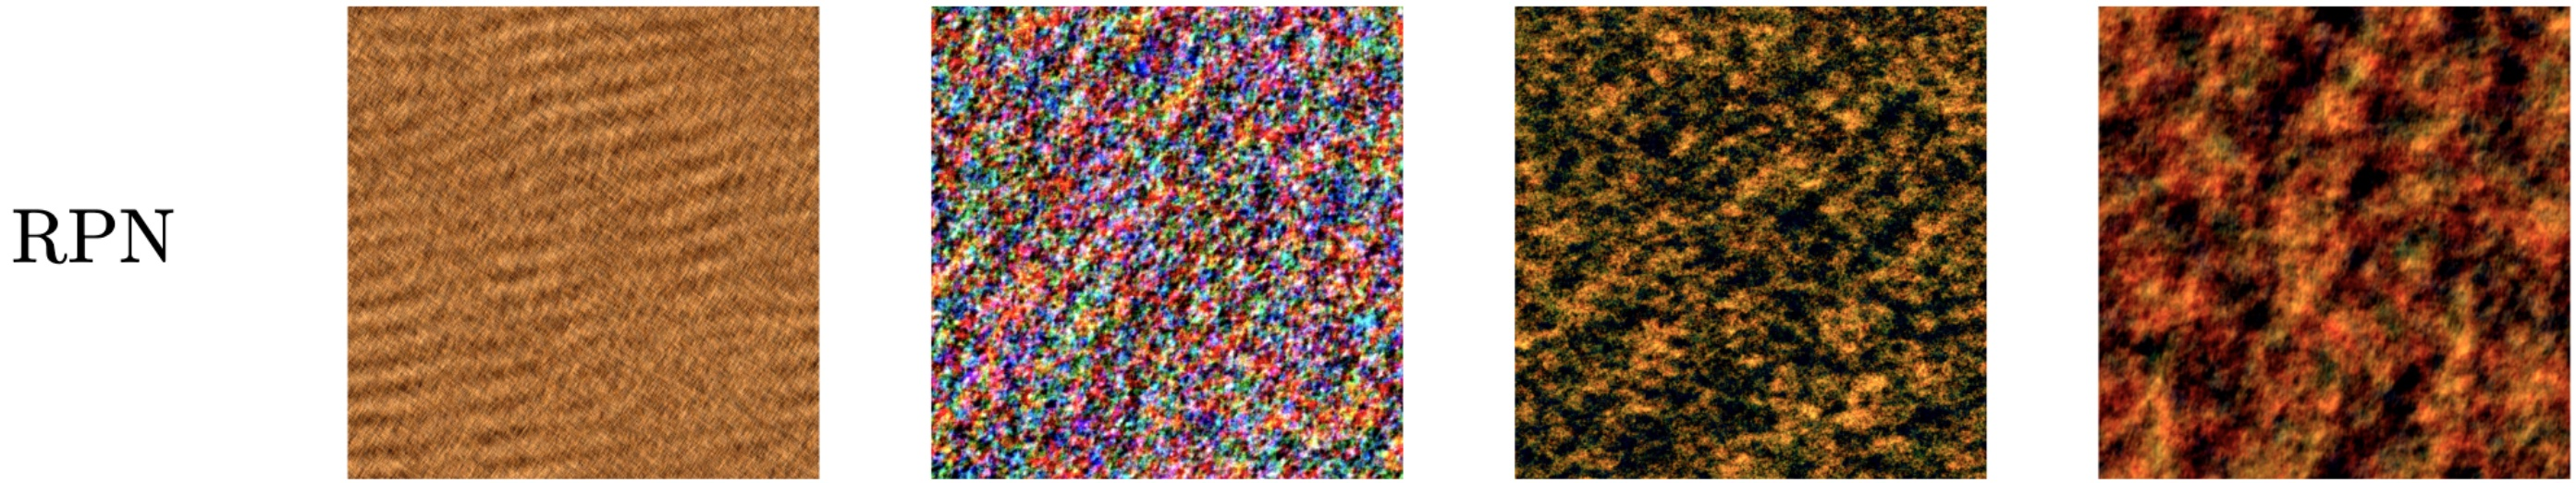
\includegraphics[width=\textwidth]{images/02-big_comparison_rpn_compressed.jpg}
        \caption*{}
        %\label{}
    \end{subfigure}
    
    \begin{subfigure}[b]{\textwidth}
        \centering
        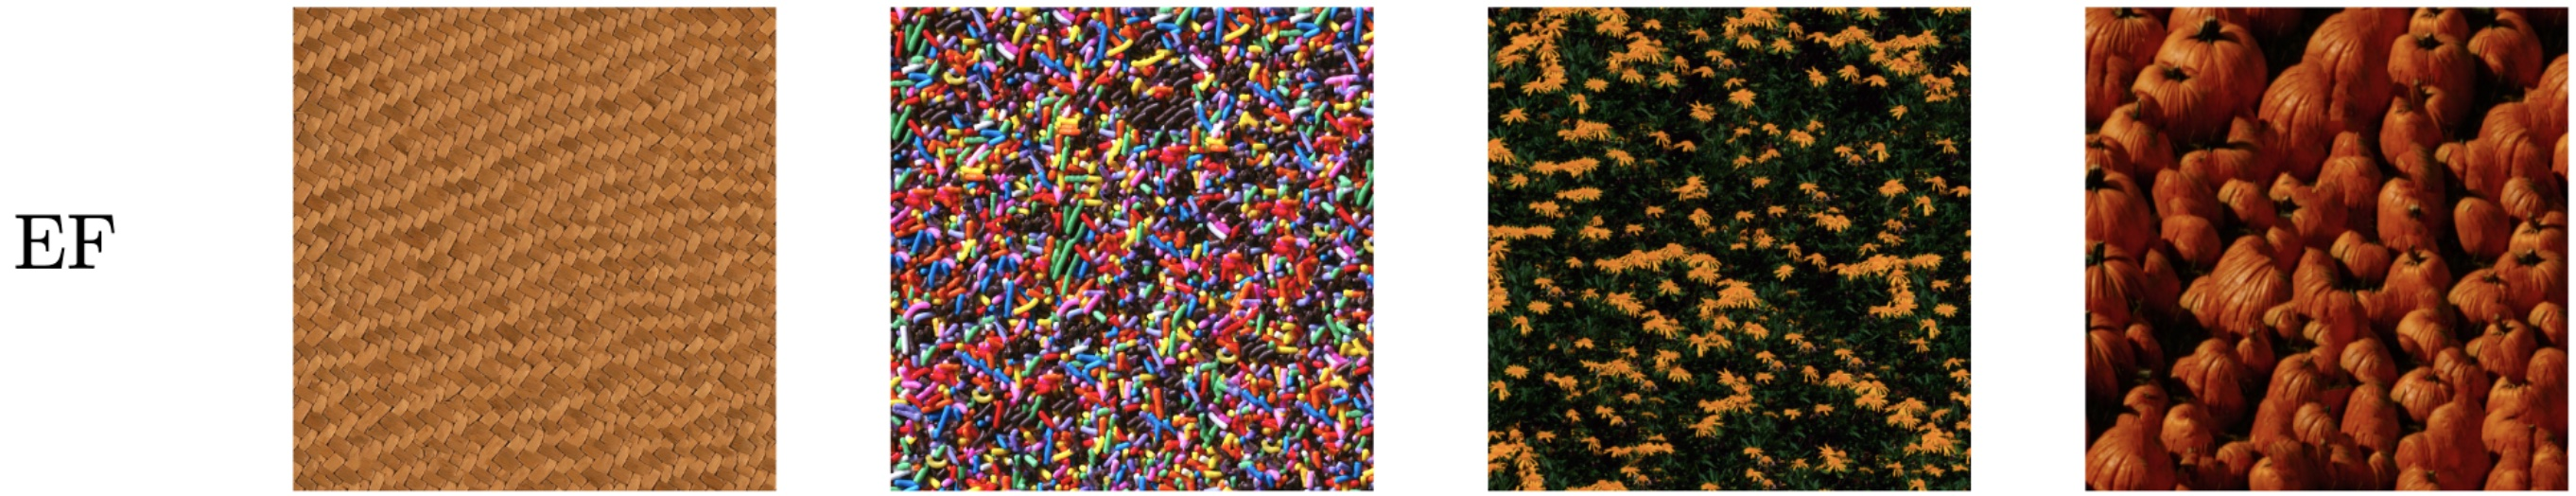
\includegraphics[width=\textwidth]{images/02-big_comparison_quilting_compressed.jpg}
        \caption*{}
        %\label{}
    \end{subfigure}

    \begin{subfigure}[b]{\textwidth}
        \centering
        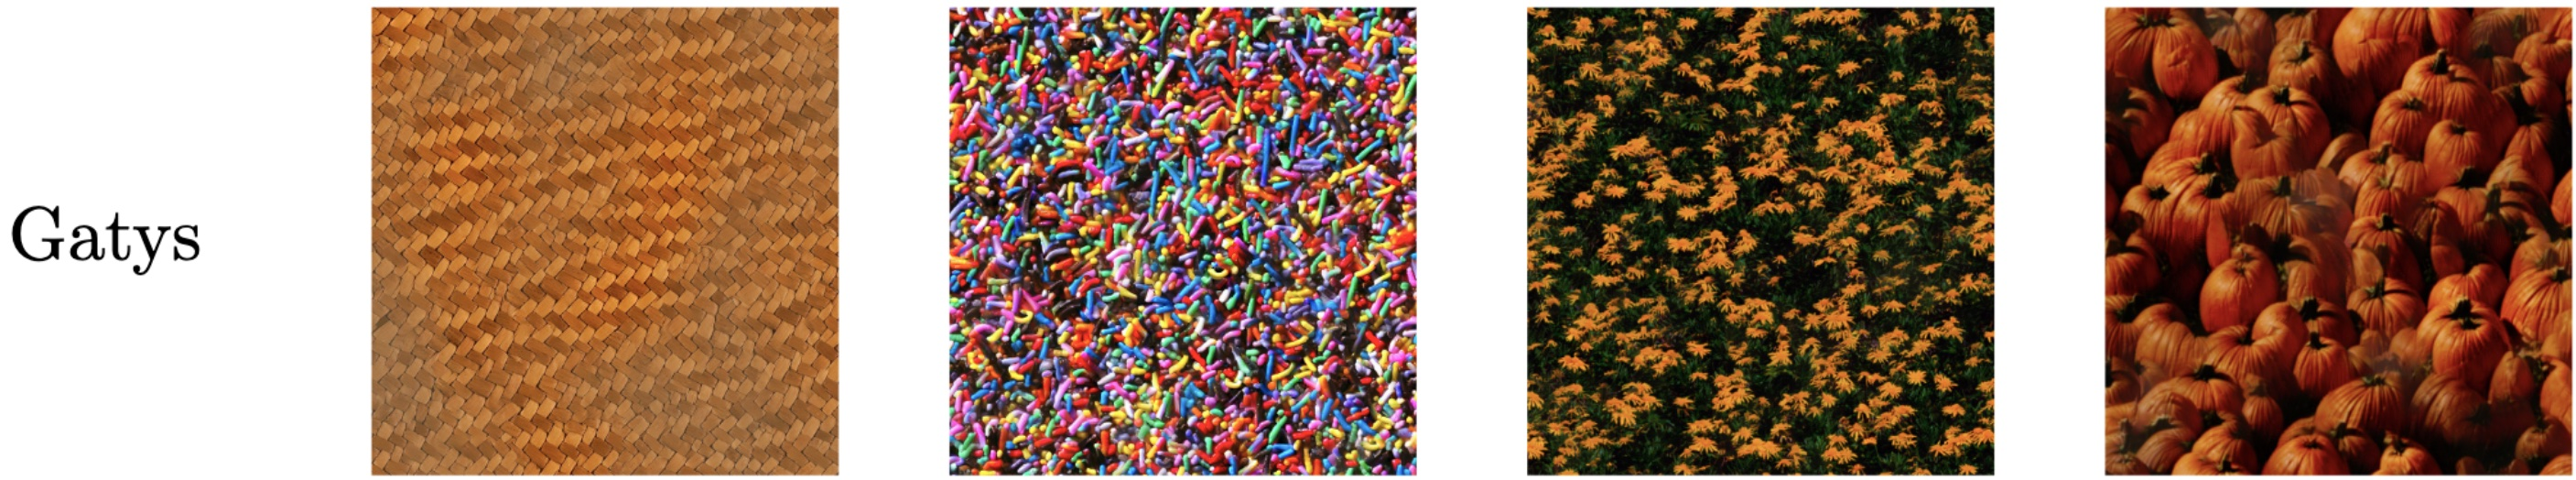
\includegraphics[width=\textwidth]{images/02-big_comparison_gatys_compressed.jpg}
        \caption*{}
        %\label{}
    \end{subfigure}
    \caption{A comparison of Gatys synthesis, Random Phase Noise (RPN, \citet{Galerne2011}) and image quilting (EF, \citet{Efros2001}). The chosen input textures are not very suitable for synthesis with Random Phase Noise as they contain fairly large features. Image quilting and Gatys seem to perform much better. Upon closer inspection, we can see that Gatys suffers from desaturated artifacts in the leftmost texture. Also, Gatys sometimes creates implausible shapes (e.g. deformed flower blooms). On the other hand, it is statistically closer to the input than EF (e.g. the flower texture generated by EF has too few blooms). Source: \citet{Raad2018}}
    \label{fig:background_synthesis_comparison}
\end{figure}

This method of synthesizing textures leads to high-quality results for a large variety of input images. Compared to patch-based synthesis it also provides a texture model, as opposed to a mere algorithm to generate new textures. This makes it easier to reason about and provide theoretical justifications as to why it works. Fig. \ref{fig:background_synthesis_comparison} taken from \citet{Raad2018} compares this method to others that we have discussed here and highlights their relative strengths and weaknesses.

\subsubsection{Potential Usage in Projection Mapping}
\label{section:background-texture_synthesis-statistics_based-projection_mapping}

This method can easily be adapted to projection mapping by modifying the optimization pipeline. The idea is to first project initial white noise image onto a scene using a differentiable rendering function. Then the resulting camera image would be fed into the CNN and ultimately compared against the input texture image. The loss gradients would flow through both the CNN and the rendering function to update the initial image. The result of this process would be an image would look like a new example of the input texture once projected.

\chapter{Environment}
\label{chapter:environment}

A problem instance is rarely totally independent of its environment.
Most often you need to describe the environment you work in, what
limits there are and so on. This is a good place to do that. Sometimes
the environment is described together with your own implemantation, in
the same chapter. Here, we first tell you about the LaTeX working
environments and then we have an example from an thesis written some years
ago.


\section{LaTeX working environments}
\label{section:environments}

To create \LaTeX\ documents you need two things: a \LaTeX\ environment for
compiling your documents and a text editor for writing them.

\subsection{Environment}

Fortunately \LaTeX\ can nowadays be found for any (modern) computer
environment, be it Linux, Windows, or Macintosh.
For Linuxes (and other Unix clones) and Macs, I'd recommend \emph{TeX
Live}~\cite{TeXLive}, which is the current default \LaTeX\ distribution for
many Linux flavors such as Fedora, Debian, Ubuntu, and Gentoo.
TeX Live is the replacement for the older \emph{teTeX}, which is
no longer developed. For Macintosh, this environment is called \emph{MacTeX}.

TeX Live works also for Windows machines (at least according to their web
site); however, I have used \emph{MiKTeX}~\cite{MiKTeX} and can recommend it
for Windows. 
MiKTeX has a nice package manager and automatically fetches missing packages
for you. There are also web service environments, for example
Sharelatex (\url{https://www.sharelatex.com/}) is available with low
or no fee for students.

\subsection{Editor}

You can write \LaTeX\ documents with any text editor you like, but having
syntax coloring options and such really helps a lot.
My personal favourite for editing \LaTeX\ is the
\emph{TeXlipse}~\cite{TeXlipse} plugin for the Eclipse IDE~\cite{Eclipse}. 
Eclipse is an open-source integrated development environment (IDE) initially
created for writing Java code, but it currently has support for editing
languages such as C, C++, JavaScript, XML, HTML, and many more. 
The TeXlipse plugin allows you to edit and compile \LaTeX\ documents directly
in Eclipse, and compilation errors and warnings are shown in the Eclipse
\emph{Problems} dialog so that you can locate and fix the issues easily.
The plugin also supports reference traversal so that you can locate the source
line where a label or a citation is defined.

Eclipse is an entire development environment, so it may feel a bit heavy-weight
for editing a document. 
If you are looking for a more light-weight option, check out TeXworks. 
TeXworks is a \LaTeX\ editor that is packaged with the newer MiKTeX
distributions, and it can be acquired from \url{http://www.tug.org/texworks/}.

And if you are attached to your \emph{emacs} or \emph{vim} editor, you
can of course edit your \LaTeX\ documents with them. 
Emacs at least has syntax coloring and you can compile your document with a key
binding, so this may be a good option if you prefer working with the standard
Linux text editors.

\section{Graphics}

When you use \texttt{pdflatex} to render your thesis, you can include
PDF images directly, as shown by Figure~\ref{fig:indica_model}
below. You can also include JPEG or PNG files, as shown by
Figure~\ref{fig:eeyore}.

\begin{figure}[ht]
  \begin{center}
    % below the size of the figure has been reduced for example
    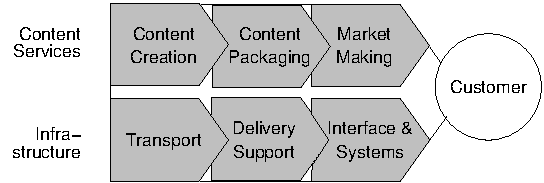
\includegraphics[width=0.80\textwidth]{images/indica_model.pdf} 
    \caption{The INDICA two-layered value chain model.}
    \label{fig:indica_model}
  \end{center}
\end{figure}


\begin{figure}[ht]
  \begin{center}
    % here the width of the figure is set to 9 cm
    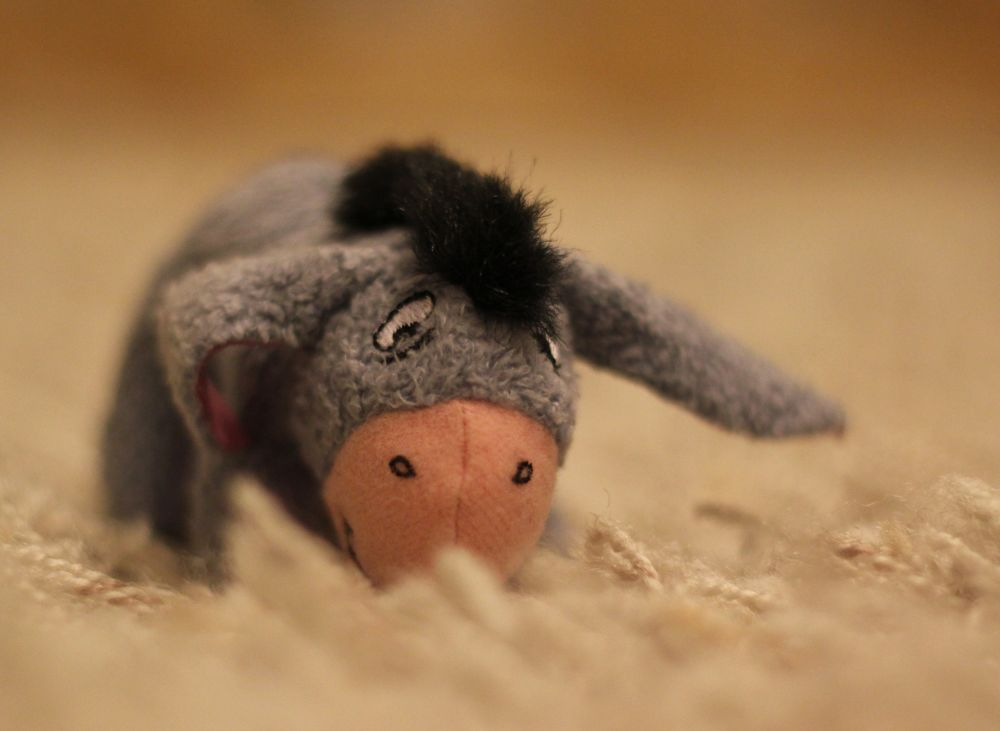
\includegraphics[width=9cm]{images/ihaa.jpg}
    \caption{Eeyore, or Ihaa, a very sad donkey.}
    \label{fig:eeyore}
  \end{center}
\end{figure}

You can create PDF files out of practically anything.  In Windows, you
can download PrimoPDF or CutePDF (or some such) and install a printing
driver so that you can print directly to PDF files from any
application. There are also tools that allow you to upload documents
in common file formats and convert them to the PDF format.  If you
have PS or EPS files, you can use the tools \texttt{ps2pdf} or
\texttt{epspdf} to convert your PS and EPS files to PDF\@.

% Comment: If your sentence ends in a capital letter, like here, you should
% write \@ before the period; otherwise LaTeX will assume that this is not
% really an end of the sentence and will not put a large enough space after the
% period. That is, LaTeX assumes that you are (for example), enumerating using
% capital roman numerals, like I. do something, II. do something else. In this
% case, the periods do not end the sentence.

% Similarly, if you do need a normal space after a period (instead of
% the longer sentence separator), use \  (backslash and space) after the
% period. Like so: a.\ first item, b.\ second item.

Furthermore, most newer editor programs allow you to save directly to the PDF
format. For vector editing, you could try Inkscape, which is a new open source
WYSIWYG vector editor that allows you to save directly to PDF\@. 
For graphs, either export/print your graphs from OpenOffice Calc/Microsoft
Excel to PDF format, and then add them; or use \texttt{gnuplot}, which can
create PDF files directly (at least the new versions can).
The terminal type is \emph{pdf}, so the first line of your plot file should be
something like \texttt{set term pdf \ldots}.

To get the most professional-looking graphics, you can encode them using the
TikZ package (TikZ is a frontend for the PGF graphics formatting system).
You can create practically any kind of technical images with TikZ, but it has a
rather steep learning curve. Locate the manual (\texttt{pgfmanual.pdf}) from
your \LaTeX\ distribution and check it out. An example of TikZ-generated
graphics is shown in Figure~\ref{fig:page-merge}.

\begin{figure}[ht]
  \begin{center}
    \newcommand*{\actver}{\smash{\ensuremath{v_{\text{\textit{active}}}}}}

\tikzstyle{lbl}=[font=\scriptsize,midway,sloped]
\tikzstyle{opendash}=[densely dotted,thick] 
\tikzstyle{opendeco}=[decoration={zigzag,amplitude=0.1em,segment length=0.6em}]
\tikzstyle{actverline}=[dashed]
\tikzstyle{entryline}=[densely dotted]
\tikzstyle{area}=[ellipse,draw,dashed]
\tikzstyle{liveentry}=[entryline,postaction={%
  decorate,%
  decoration={%
    markings,%
    mark=at position .5pt with{\arrowreversed[line width=.35pt]{|}};,
    mark=at position 1 with{%
      \arrow[line width=.8pt]{stealth}};%
  }%
}]
\tikzstyle{deadentry}=[entryline,postaction={%
  decorate,%
  decoration={%
    markings,%
    mark=at position .5pt with{\arrowreversed[line width=.35pt]{|}};,
    mark=at position 1 with{%
      \arrow[line width=.8pt]{stealth}};%
%      \arrow[line width=.35pt,black,fill=white]{*}};% 
  }%
}]
\tikzstyle{pageborder}=[thick]
\tikzstyle{pagename}=[anchor=center,text=black!50,font=\huge]
\newlength{\spexx}
\setlength{\spexx}{1.2cm}
\newlength{\spexy}
\setlength{\spexy}{.5cm}

\subfigure[Before]{
\begin{tikzpicture}[x=\spexx,y=\spexy,%
  every pin edge/.style={draw,dotted},%
  pin distance=.5\spexx]
  \small
  \coordinate (lo) at (0,-5);
  \coordinate (o) at (0,0);
  \coordinate (hi) at (0,7);
  \coordinate (loact) at (3,-5);
  \coordinate (oact) at (3,0);
  \coordinate (hiact) at (3,7);
  \coordinate (loinf) at (4,-5);
  \coordinate (oinf) at (4,0);
  \coordinate (hiinf) at (4,7);
  
  \draw[->] (lo) -- node[below,lbl] {Versions} ($(loinf) + (1em,0)$);
  \draw[->] (lo) -- node[above,lbl] {Keys} ($(hi) + (0,1em)$);

  \draw[pageborder] (lo) -- (o) -- (hi);
  \draw[pageborder] (lo) -- (loinf);
  \draw[pageborder] (hi) -- (hiinf);
  \draw[pageborder] (o) -- (oinf);

  \draw[opendash] decorate [opendeco] { (loinf) -- (oinf) };
  \draw[opendash] decorate [opendeco] { (oinf) -- (hiinf) };

  \node[pagename] at (2,3.5) {$p$};
  \node[pagename] at (2,-2.5) {$s$};

  \draw[actverline] ($(loact) + (0,-1em)$) node[below=.4em] {\actver} --
    ($(hiact) + (0,1em)$);

  % Page p contents
  \draw[deadentry] (0,6) -- (1,6);
  \draw[deadentry] (1,6) -- (2,6);
  \draw[deadentry] (2,6) -- (3,6);
  \draw[liveentry] (0,5) -- (4,5);
  \draw[deadentry] (0,4) -- (2,4);
  \draw[deadentry] (1,3) -- (3,3);
  \draw[deadentry] (0,2) -- (1,2);
  \draw[deadentry] (2,2) -- (3,2);
  \draw[deadentry] (0,1) -- (2,1);
  \draw[deadentry] (2,1) -- (3,1);

  % Page s contents
  \draw[liveentry] (0,-1) -- (4,-1);
  \draw[deadentry] (0,-2) -- (2,-2);
  \draw[deadentry] (0,-3) -- (3,-3);
  \draw[liveentry] (3,-4) -- (4,-4);

  \node[area,minimum width=4.5\spexx,minimum height=.6\spexy,pin=178:{$1$}]
    at (2,5) {};
  \node[area,minimum width=4.5\spexx,minimum height=.6\spexy,pin=182:{$2$}]
    at (2,-1) {};
  \node[area,minimum width=1.5\spexx,minimum height=.6\spexy,pin=330:{$3$}]
    at (3.5,-4) {};

\end{tikzpicture}}
\subfigure[After]{
\begin{tikzpicture}[x=\spexx,y=\spexy,%
  every pin edge/.style={draw,dotted},%
  pin distance=.5\spexx]
  \small
  \coordinate (lo) at (0,-5);
  \coordinate (o) at (0,0);
  \coordinate (hi) at (0,7);
  \coordinate (loact) at (3,-5);
  \coordinate (oact) at (3,0);
  \coordinate (hiact) at (3,7);
  \coordinate (loinf) at (4,-5);
  \coordinate (oinf) at (4,0);
  \coordinate (hiinf) at (4,7);

  \draw[->] (lo) -- node[lbl,below] {Versions} ($(loinf) + (1em,0)$);
  \draw[->] (lo) -- node[lbl,above] {Keys} ($(hi) + (0,1em)$);

  \draw[pageborder] (lo) -- (o) -- (hi);
  \draw[pageborder] (lo) -- (loinf);
  \draw[pageborder] (hi) -- (hiinf);
  \draw[pageborder] (o) -- (oact);

  \draw[opendash] decorate [opendeco] { (loinf) -- (oinf) };
  \draw[opendash] decorate [opendeco] { (oinf) -- (hiinf) };

  \node[pagename] at (1.5,3.5) {$p$};
  \node[pagename] at (1.5,-2.5) {$s$};
  \node[pagename] at (3.5,1) {$p'$};

  \draw[actverline] ($(loact) + (0,-1em)$) node[below=.4em] {\actver} -- (loact);
  \draw[pageborder] (loact) -- (hiact);
  \draw[actverline] (hiact) -- ($(hiact) + (0,1em)$);

  % Page p contents
  \draw[deadentry] (0,6) -- (1,6);
  \draw[deadentry] (1,6) -- (2,6);
  \draw[deadentry] (2,6) -- (3,6);
  \draw[deadentry] (0,5) -- (3,5);
  \draw[deadentry] (0,4) -- (2,4);
  \draw[deadentry] (1,3) -- (3,3);
  \draw[deadentry] (0,2) -- (1,2);
  \draw[deadentry] (2,2) -- (3,2);
  \draw[deadentry] (0,1) -- (2,1);
  \draw[deadentry] (2,1) -- (3,1);

  % Page s contents
  \draw[deadentry] (0,-1) -- (3,-1);
  \draw[deadentry] (0,-2) -- (2,-2);
  \draw[deadentry] (0,-3) -- (3,-3);

  % Page p' contents
  \draw[liveentry] (3,5) -- (4,5);
  \draw[liveentry] (3,-1) -- (4,-1);
  \draw[liveentry] (3,-4) -- (4,-4);

  \node[area,minimum width=1.5\spexx,minimum height=.6\spexy,pin=10:{$1$}]
    at (3.5,5) {};
  \node[area,minimum width=1.5\spexx,minimum height=.6\spexy,pin=3:{$2$}]
    at (3.5,-1) {};
  \node[area,minimum width=1.5\spexx,minimum height=.6\spexy,pin=330:{$3$}]
    at (3.5,-4) {};
\end{tikzpicture}}

    \caption{Example of a multiversion database page merge. This figure has
    been taken from the PhD thesis of Haapasalo~\cite{HaapasaloThesis}.}
    \label{fig:page-merge}
  \end{center}
\end{figure}

Another example of graphics created with TikZ is shown in
Figure~\ref{fig:tikz-examples}. 
These show how graphs can be drawn and labeled. 
You can consult the example images and the PGF manual for more examples of what
kinds figures you can draw with TikZ. 

% These definitions are only used in the example images; you will not 
% need them for your thesis...
\newlength{\graphdotsize}
\setlength{\graphdotsize}{1.7pt}
\newlength{\graphgridsize}
\setlength{\graphgridsize}{1.2em}
\begin{figure}[ht]
\begin{center}
\subfigure[Examples of obstruction graphs for the Ferry Problem]{
  \newlength{\oggs}
\setlength{\oggs}{1.2\graphgridsize}
\begin{tikzpicture}[x=\oggs,y=\oggs,every pin edge/.style={draw,dotted},pin distance=0.5\oggs,area/.style={ellipse,draw,dashed}] 

% The graph (0,0,5,0)
% o = origo
\coordinate (o) at (0,0);
\coordinate[left=1 of o,pin=100:$q_1$] (q1);
\coordinate[right=1 of o,pin=80:$q_2$] (q2);
\fill[black] (q1) circle (\graphdotsize);
\fill[black] (q2) circle (\graphdotsize);
\foreach \d in {-2, -1, ..., 2} {
  \coordinate (tmp) at ($(o) + (0,\d)$);
  \draw (q1) -- (tmp);
  \draw (q2) -- (tmp);
  \fill[black] (tmp) circle (\graphdotsize);
}
\node[area,minimum height=5.3\oggs,minimum width=0.8\oggs,pin=94:$X_3$] at (o) {};  

% The graph (1,0,3,0)
\coordinate[right=5 of o] (o);
\coordinate[left=1 of o,pin=260:$q_1$] (q1);
\coordinate[left=2 of o] (q1v);
\coordinate[right=1 of o,pin=280:$q_2$] (q2);
\fill[black] (q1) circle (\graphdotsize);
\fill[black] (q2) circle (\graphdotsize);
\fill[black] (q1v) circle (\graphdotsize);
\draw (q1) -- (q1v);
\foreach \d in {-1, 0, 1} {
  \coordinate (tmp) at ($(o) + (0,\d)$);
  \draw (q1) -- (tmp);
  \draw (q2) -- (tmp);
  \fill[black] (tmp) circle (\graphdotsize);
}
\node[area,minimum height=3.3\oggs,minimum width=0.8\oggs,pin=266:$X_3$] at (o) {};  
\node[area,minimum height=0.8\oggs,minimum width=0.8\oggs,pin=260:$X_1$] at (q1v) {};  


% The graph (0,1,3,0)
\coordinate[right=4 of o] (o);
\coordinate[left=1 of o,pin=100:$q_1$] (q1);
\coordinate[right=1 of o,pin=80:$q_2$] (q2);
\coordinate[right=2 of o] (q2v);
\fill[black] (q1) circle (\graphdotsize);
\fill[black] (q2) circle (\graphdotsize);
\fill[black] (q2v) circle (\graphdotsize);
\draw (q2) -- (q2v);
\foreach \d in {-1, 0, 1} {
  \coordinate (tmp) at ($(o) + (0,\d)$);
  \draw (q1) -- (tmp);
  \draw (q2) -- (tmp);
  \fill[black] (tmp) circle (\graphdotsize);
}
\node[area,minimum height=3.3\oggs,minimum width=0.8\oggs,pin=94:$X_3$] at (o) {};  
\node[area,minimum height=0.8\oggs,minimum width=0.8\oggs,pin=80:$X_2$] at (q2v) {};  

% The graph (0,0,3,1)
\coordinate[right=5 of o] (o);
\coordinate[left=1 of o,pin=260:$q_1$] (q1);
\coordinate[right=1 of o,pin=290:$q_2$] (q2);
\fill[black] (q1) circle (\graphdotsize);
\fill[black] (q2) circle (\graphdotsize);
\draw (q1) -- (q2);
\foreach \d in {-1, 1, 2} {
  \coordinate (tmp) at ($(o) + (0,\d)$);
  \draw (q1) -- (tmp);
  \draw (q2) -- (tmp);
  \fill[black] (tmp) circle (\graphdotsize);
}
\node[area,minimum height=4.3\oggs,minimum width=0.8\oggs,pin=266:$X_3$] at ($(o) + (0,0.5)$) {};  

\end{tikzpicture}

}
\subfigure[Examples of star graphs]{
  \begin{tikzpicture}[x=\graphgridsize,y=\graphgridsize] 

\coordinate (o) at (0,0);
\fill[black] (o) circle (\graphdotsize);
\foreach \d in {0, 90, ..., 270} {
  \coordinate (tmp) at ($(o) + (\d:1.5)$);
  \draw (o) -- (tmp);
  \fill[black] (tmp) circle (\graphdotsize);
}

\coordinate[right=4 of o] (o);
\coordinate (o1) at ($(o) + (0:0.3)$);
\coordinate (o2) at ($(o) + (180:0.3)$);
\fill[black] (o1) circle (\graphdotsize);
\fill[black] (o2) circle (\graphdotsize);
\draw (o1) -- (o2);
\foreach \d in {45, 135, 270} {
  \coordinate (tmp\d) at ($(o) + (\d:1.5)$);
  \draw (o2) -- (tmp\d);
  \fill[black] (tmp\d) circle (\graphdotsize);
}
\draw (o1) -- (tmp45);


\coordinate[right=4 of o] (o);
\coordinate (o1) at ($(o) + (0:0.3)$);
\coordinate (o2) at ($(o) + (180:0.3)$);
\fill[black] (o1) circle (\graphdotsize);
\fill[black] (o2) circle (\graphdotsize);
\draw (o1) -- (o2);
\foreach \d in {45, 135, 270} {
  \coordinate (tmp\d) at ($(o) + (\d:1.5)$);
  \draw (o2) -- (tmp\d);
  \fill[black] (tmp\d) circle (\graphdotsize);
}
\draw (o1) -- (tmp45);
\draw (o1) -- (tmp135);


\coordinate[right=4 of o] (o);
\coordinate (o1) at ($(o) + (0:0.3)$);
\coordinate (o2) at ($(o) + (180:0.3)$);
\fill[black] (o1) circle (\graphdotsize);
\fill[black] (o2) circle (\graphdotsize);
\draw (o1) -- (o2);
\foreach \d in {45, 135, 270} {
  \coordinate (tmp\d) at ($(o) + (\d:1.5)$);
  \draw (o1) -- (tmp\d);
  \draw (o2) -- (tmp\d);
  \fill[black] (tmp\d) circle (\graphdotsize);
}


\coordinate[right=3.5 of o] (o);
\coordinate (o1) at ($(o) + (90:0.3)$);
\coordinate (o2) at ($(o) + (210:0.5)$);
\coordinate (o3) at ($(o) + (330:0.5)$);
\fill[black] (o1) circle (\graphdotsize);
\fill[black] (o2) circle (\graphdotsize);
\fill[black] (o3) circle (\graphdotsize);
\draw (o1) -- (o2);
\draw (o1) -- (o3);
\draw (o2) -- (o3);
\foreach \d in {90, 270} {
  \coordinate (tmp\d) at ($(o) + (\d:1.5)$);
  \draw (o2) -- (tmp\d);
  \draw (o3) -- (tmp\d);
  \fill[black] (tmp\d) circle (\graphdotsize);
}
\draw (o1) -- (tmp90);


\coordinate[right=3 of o] (o);
\coordinate (o1) at ($(o) + (90:0.3)$);
\coordinate (o2) at ($(o) + (210:0.5)$);
\coordinate (o3) at ($(o) + (330:0.5)$);
\fill[black] (o1) circle (\graphdotsize);
\fill[black] (o2) circle (\graphdotsize);
\fill[black] (o3) circle (\graphdotsize);
\draw (o1) -- (o2);
\draw (o1) -- (o3);
\draw (o2) -- (o3);
\foreach \d in {90, 270} {
  \coordinate (tmp\d) at ($(o) + (\d:1.5)$);
  \draw (o2) -- (tmp\d);
  \draw (o3) -- (tmp\d);
  \fill[black] (tmp\d) circle (\graphdotsize);
}
\draw (o1) -- (tmp90);
\draw (o1) -- (tmp270);



\coordinate[right=3.5 of o] (o);
\coordinate (o1) at ($(o) + (18:1.3)$);
\coordinate (o2) at ($(o) + (90:1.3)$);
\coordinate (o3) at ($(o) + (162:1.3)$);
\coordinate (o4) at ($(o) + (234:1.3)$);
\coordinate (o5) at ($(o) + (306:1.3)$);
\foreach \d in {1, 2, ..., 5} {
  \fill[black] (o\d) circle (\graphdotsize);
}
\draw (o1) -- (o2);
\draw (o1) -- (o3);
\draw (o1) -- (o4);
\draw (o1) -- (o5);
\draw (o2) -- (o3);
\draw (o2) -- (o4);
\draw (o2) -- (o5);
\draw (o3) -- (o4);
\draw (o3) -- (o5);
\draw (o4) -- (o5);

\end{tikzpicture}

}
\caption{Examples of graphs draw with TikZ. These figures have been taken from a
course report for the graph theory course~\cite{FerryProblem}.}
\label{fig:tikz-examples}
\end{center}
\end{figure}

\section{Compilation}
\label{section:compilation}

After you have written your text, you have to compile your *.tex files to get 
a pdf presentation. Use pdflatex to compile, because the input images are expected 
as PDF files. Your \LaTeX environment can provide the compiling tool, too.

An example how to compile your thesis:
\begin{itemize}
	% You can use this command to set the items in the list closer to each other
	% (ITEM SEParation, the vertical space between the list items) 
	\setlength{\itemsep}{5pt}
	\item pdflatex thesis-example.tex
	\item bibtex thesis-example
	\item pdflatex thesis-example.tex
	\item pdflatex thesis-example.tex
\end{itemize}

You need to run pdflatex multiple times, so that all the cross-references
are fixed. Pdflatex will tell you, if you need to re-run it (a warning
will be issued).  

The compilation has been tested to work in kosh.aalto.fi, in an Ubuntu operating
system with TeX Live, in an Arch Linux, in a Mac (OSX) with MacTex and
TeXShop, and also in 
an online LaTeX editor ShareLaTeX. If you have problems of missing .sty -files, 
when compiling, then the local LaTeX environment does not have all the 
required packages installed.



\chapter{Methods}
\label{chapter:methods}

You have now stated your problem, and you are ready to do something
about it!  \emph{How} are you going to do that? What methods do you
use?  You also need to review existing literature to justify your
choices, meaning that why you have chosen the method to be applied in
your work.

% An example of a traditional LaTeX table
% ------------------------------------------------------------------
% A note on underfull/overfull table cells and tables:
% ------------------------------------------------------------------
% In professional typography, the width of the text in a page is always a lot
% less than the width of the page. If you are accustomed to the (too wide) text
% areas used in Microsoft Word's standard documents, the width of the text in
% this thesis layout may suprise you. However, text in a book needs wide
% margins. Narrow text is easier to read and looks nicer. Longer lines are 
% hard to read, because the start of the next line is harder to locate when
% moving from line to the next. 
% However, tables that are in the middle of the text often would require a wider
% area. By default, LaTeX will complain if you create too wide tables with
% ``overfull'' error messages, and the table will not be positioned properly
% (not centered). If at all possible, try to make the table narrow enough so
% that it fits to the same space as the text (total width = \textwidth).
% If you do need more space, you can either
% 1) ignore the LaTeX warnings 
% 2) use the textpos-package to manually position the table (read the package
%    documentation)
% 3) if you have the table as a PDF document (of correct size, A4), you can use
%    the pdfpages package to include the page. This overrides the margin
%    settings for this page and LaTeX will not complain.
% ------------------------------------------------------------------
% Another note:
% ------------------------------------------------------------------
% If your table fits to \textwidth, but the cells are so narrow that the text
% in p{..}-formatted cells does not flow nicely (you get underfull warnings 
% because LaTeX tries to justify the text in the cells) you can manually set
% the text to unjustified by using the \raggedright command for each cell 
% that you do not want to be justified (see the example below). \raggedleft 
% is also possible, of course...
% ------------------------------------------------------------------
% If you need to have linefeeds (\\) inside a cell, you must create a new
% paragraph-formatting environment inside the cell. Most common ones are 
% the minipage-environment and the \parbox command (see LaTeX documentation
% for details; or just google for ``LaTeX minipage'' and ``LaTeX parbox'').
\begin{table}
\begin{tabular}{|p{2cm}|p{3.5cm}|p{4.2cm}|p{1.8cm}|} 
% Alignment of sells: l=left, c=center, r=right. 
% If you want wrapping lines, use p{width} exact cell widths.
% If you want vertical lines between columns, write | above between the letters
% Horizontal lines are generated with the \hline command:
\hline % The line on top of the table
\textbf{Code} & \textbf{Name} & \textbf{Methods} & \textbf{Area} \\ 
\hline 
% Place a & between the columns
% In the end of the line, use two backslashes \\ to break the line,
% then place a \hline to make a horizontal line below the row 
CS-E4900 & User-Centered Methods for Product and Service Design
    & \raggedright Interviews, observations, questionnaires, probes, etc
& Usability \\ 
\hline
\multicolumn{2}{|p{6.25cm}|}{MS-E2108 Simulation (here is an example of
 multicolumn for tables)}& Details of how to build simulations &
                                                                 Computer Science \\
% The multicolumn command takes the following 3 arguments: 
% the number of cells to merge, the cell formatting for the new cell, and the
% contents of the cell
\hline
ELEC-E7130 & Internet Traffic Measurements and Analysis 
& \raggedright How to measure and analyse network
  traffic & Communi\-cations \\ \hline % here we give hint for hyphenation
\end{tabular} % for really simple tables, you can just use tabular
% You can place the caption either below (like here) or above the table
\caption{Research methodology courses}
% Place the label just after the caption to make the link work
\label{table:courses}
\end{table} % table makes a floating object with a title

If you have not yet done any (real) metholodogical courses, 
now is the time to do so or at least
check through material of suitable methodological courses. Some
methodologial courses that consentrates especially to methods in
different fields of computer science are
presented in Table~\ref{table:courses}. Remember to explain the
content of the tables (as with figures). In the table, the last column
gives the research area where the methods are often used. 

Here we used table to give an example of tables, and you can read more
about tables from the latex source file \texttt{4methods.tex}. In the
beginning of the thesis, the section Abbreviations and Acronyms is
also a long table. The difference is that longtables can continue to
next page.


 
\chapter{Implementation}
\label{chapter:implementation}

You have now explained how you are going to tackle your problem. 
Go do that now! Come back when the problem is solved!

Now, how did you solve the problem? 
Explain how you implemented your solution, be it a software component, a
custom-made FPGA, a fried jelly bean, or whatever.
Describe the problems you encountered with your implementation
work. Sometimes the content of the environment chapter is combined
together with the implementation chapter.



\chapter{Evaluation}
\label{chapter:evaluation}

You have done your work, but that's\footnote{By the way, do \emph{not} use
shorthands like this in your text! It is not professional! Always write out all
the words: ``that is''.} not enough. 

You also need to evaluate how well your implementation works.  The
nature of the evaluation depends on your problem, your method, and
your implementation that are all described in the thesis before this
chapter.  If you have created a program for exact-text matching, then
you measure how long it takes for your implementation to search for
different patterns, and compare it against the implementation that was
used before.  If you have designed a process for managing software
projects, you perhaps interview people working with a waterfall-style
management process, have them adapt your management process, and
interview them again after they have worked with your process for some
time. See what's changed.

The important thing is that you can evaluate your success somehow.
Remember that you do not have to succeed in making something spectacular; a
total implementation failure may still give grounds for a very good master's
thesis---if you can analyze what went wrong and what should have been
done. 

 

 
\chapter{Discussion}
\label{chapter:discussion}

At this point, you will have some insightful thoughts on your
implementation and you may have ideas on what could be done in the
future. This chapter may be combined together with the evaluation
chapter. All the new insights and findings are given here!  This
chapter is a good place to discuss your thesis as a whole and to show
your professor that you have really understood some non-trivial
aspects of the methods you used\ldots


 
\chapter{Conclusions}
\label{chapter:conclusions}

Time to wrap it up!  Write down the most important findings from your
work.  Like the introduction, this chapter is not very long.  One to
two (never over three) pages might be a good limit. Still, the chapter
gives the background, goals, content, and the findings. However, all that
should already be in the previous chapters. This is just a summary (as
are the abstract and the introduction).

For making PDF/A version requested by the Aalto Library, open the end result pdf file in Acrobat and store it as PDF/A. Then verify the result (everything should be fine, at least as PDF/A-2b version works).

Congratulations, your thesis is ready and it looks beautiful!



% Load the bibliographic references
% ------------------------------------------------------------------
% You can use several .bib files:
% \bibliography{thesis_sources,ietf_sources}
\bibliography{sources}


% Appendices go here
% ------------------------------------------------------------------
% If you do not have appendices, comment out the following lines
\appendix
\chapter{First appendix}
\label{chapter:first-appendix}

This is the first appendix. You could put some test images or verbose data in an
appendix, if there is too much data to fit in the actual text nicely.

For now, the Aalto logo variants are shown in Figure~\ref{fig:aaltologo}.

\begin{figure}
\begin{center}
\subfigure[In English]{
\includegraphics[width=.8\textwidth]{images/aalto-logo-en}}
\subfigure[Suomeksi]{
\includegraphics[width=.8\textwidth]{images/aalto-logo-fi}}
\subfigure[P� svenska]{
\includegraphics[width=.8\textwidth]{images/aalto-logo-se}}
\caption{Aalto logo variants}
\label{fig:aaltologo}
\end{center}
\end{figure}


% End of document!
% ------------------------------------------------------------------
% The LastPage package automatically places a label on the last page.
% That works better than placing a label here manually, because the
% label might not go to the actual last page, if LaTeX needs to place
% floats (that is, figures, tables, and such) to the end of the 
% document.
\end{document}
